%%%%%%%%%%%%%%%%%%%%%%%%%%%%%%%%%%%%%%%%%
% Classicthesis Typographic Thesis
% LaTeX Template
% Version 1.1 (4/8/12)
%
% This template has been downloaded from:
% http://www.LaTeXTemplates.com
%
% Original author:
% André Miede (http://www.miede.de)
%
% License:
% CC BY-NC-SA 3.0 (http://creativecommons.org/licenses/by-nc-sa/3.0/)
%
% General Tips:
% 1) Make sure to edit the classicthesis-config.file
% 2) New enumeration (A., B., C., etc in small caps): \begin{aenumerate} \end{aenumerate}
% 3) For margin notes: \marginpar or \graffito{}
% 4) Do not use bold fonts in this style, it is designed around them
% 5) Use tables as in the examples
% 6) See classicthesis-preamble.sty for useful commands
%
%%%%%%%%%%%%%%%%%%%%%%%%%%%%%%%%%%%%%%%%%

%----------------------------------------------------------------------------------------
%	PACKAGES AND OTHER DOCUMENT CONFIGURATIONS
%----------------------------------------------------------------------------------------
\documentclass[letterpaper,
		oneside,openright,titlepage,numbers=noenddot,headinclude,%1headlines,
                footinclude=true, cleardoublepage=empty,
                BCOR=5mm,paper=letterpaper,fontsize=11pt, % Binding correction, paper type and font size
                ngerman,american, % Languages
                ]{scrreprt} 
                
                
% Includes the file which contains all the document configurations and packages - make sure to edit this file
%%%%%%%%%%%%%%%%%%%%%%%%%%%%%%%%%%%%%%%%%
% Thesis Configuration File
%
% The main lines to change in this file are in the DOCUMENT VARIABLES
% section, the rest of the file is for advanced configuration.
%
%%%%%%%%%%%%%%%%%%%%%%%%%%%%%%%%%%%%%%%%%

%----------------------------------------------------------------------------------------
%	DOCUMENT VARIABLES
%	Fill in the lines below to enter your information into the thesis template
%	Each of the commands can be cited anywhere in the thesis
%----------------------------------------------------------------------------------------

% Remove drafting to get rid of the '[ Date - classicthesis version 4.0 ]' text at the bottom of every page
\PassOptionsToPackage{eulerchapternumbers,listings, pdfspacing, subfig,beramono,eulermath,parts,dottedtoc}{classicthesis}
% Available options: drafting parts nochapters linedheaders eulerchapternumbers beramono eulermath pdfspacing minionprospacing tocaligned dottedtoc manychapters listings floatperchapter subfig
% Adding 'dottedtoc' will make page numbers in the table of contents flushed right with dots leading to them

\newcommand{\myTitle}{A Model for Evaluating Player Experience in Rehabilitation Exergames\xspace}
\newcommand{\mySubtitle}{Project Proposal\xspace}
\newcommand{\myDegree}{}
\newcommand{\myName}{Edwin Gamboa, Eng.\xspace}
\newcommand{\myCode}{201700750\xspace}
\newcommand{\myEmail}{edwin.gamboa@correounivalle.edu.co\xspace}
\newcommand{\myProf}{}
\newcommand{\myOtherProf}{}
\newcommand{\myAdvisor}{Maria Trujillo, PhD.\xspace}
\newcommand{\myFaculty}{Facultad de Ingenier\'ia\xspace}
\newcommand{\myDepartment}{Escuela de Ingenier\'ia de Sistemas y Computaci\'on\xspace}
\newcommand{\myUni}{Universidad del Valle\xspace}
\newcommand{\myLocation}{Cali, Colombia\xspace}
\newcommand{\myTime}{August 2018\xspace}
\newcommand{\myVersion}{version 1.0\xspace}

%----------------------------------------------------------------------------------------
%	USEFUL COMMANDS
%----------------------------------------------------------------------------------------

\newcommand{\ie}{i.\,e.\xspace}
\newcommand{\Ie}{I.\,e.\xspace}
\newcommand{\eg}{e.\,g.\xspace}
\newcommand{\Eg}{E.\,g.\xspace} 

\newcounter{dummy} % Necessary for correct hyperlinks (to index, bib, etc.)
\providecommand{\mLyX}{L\kern-.1667em\lower.25em\hbox{Y}\kern-.125emX\@}

%----------------------------------------------------------------------------------------
%	PACKAGES
%----------------------------------------------------------------------------------------

\usepackage{lipsum} % Used for inserting dummy 'Lorem ipsum' text into the template

%------------------------------------------------
 
\PassOptionsToPackage{latin9}{inputenc} % latin9 (ISO-8859-9) = latin1+"Euro sign"
\usepackage[utf8]{inputenc}
 
%------------------------------------------------
\usepackage{float} %Usar etiqueta H
%------------------------------------------------

%\PassOptionsToPackage{ngerman,american}{babel}  % Change this to your language(s)
% Spanish languages need extra options in order to work with this template
%\PassOptionsToPackage{spanish,es-lcroman}{babel}
\usepackage{babel}

%------------------------------------------------			

%\PassOptionsToPackage{square,numbers}{natbib}
%\usepackage{natbib}

\usepackage{csquotes}
\usepackage[
style=numeric-comp,
backend=biber,
sorting=none
]{biblatex}
%\DeclareLanguageMapping{american}{american-apa}
\addbibresource{Bibliography.bib}


 
 %------------------------------------------------

\PassOptionsToPackage{fleqn}{amsmath} % Math environments and more by the AMS 
 \usepackage{amsmath}
 
 %------------------------------------------------

\PassOptionsToPackage{T1}{fontenc} % T2A for cyrillics
\usepackage{fontenc}

%------------------------------------------------

\usepackage{xspace} % To get the spacing after macros right

%------------------------------------------------

\usepackage{mparhack} % To get marginpar right

%------------------------------------------------

\usepackage{fixltx2e} % Fixes some LaTeX stuff 

%------------------------------------------------

\PassOptionsToPackage{smaller}{acronym} % Include printonlyused in the first bracket to only show acronyms used in the text
\usepackage{acronym} % nice macros for handling all acronyms in the thesis

%------------------------------------------------

%\renewcommand*{\acsfont}[1]{\textssc{#1}} % For MinionPro
\newcommand{\bflabel}[1]{{#1}\hfill} % Fix the list of acronyms

%------------------------------------------------

\PassOptionsToPackage{pdftex}{graphicx}
\usepackage{graphicx}
\usepackage[export]{adjustbox}
\usepackage[lofdepth,lotdepth]{subfig}

%----------------------------------------------------------------------------------------
%	FLOATS: TABLES, FIGURES AND CAPTIONS SETUP
%----------------------------------------------------------------------------------------

\usepackage{tabularx} % Better tables
\setlength{\extrarowheight}{2pt} % Increase table row height
\newcommand{\tableheadline}[1]{\multicolumn{1}{c}{\spacedlowsmallcaps{#1}}}
\newcommand{\myfloatalign}{\centering} % To be used with each float for alignment
\usepackage{caption}
\captionsetup{format=hang,font=small}
\usepackage{subfig}  

%----------------------------------------------------------------------------------------
%	CODE LISTINGS SETUP
%----------------------------------------------------------------------------------------

\usepackage{listings} 
%\lstset{emph={trueIndex,root},emphstyle=\color{BlueViolet}}%\underbar} % for special keywords
\lstset{language=[LaTeX]Tex, % Specify the language for listings here
keywordstyle=\color{RoyalBlue}, % Add \bfseries for bold
basicstyle=\small\ttfamily, % Makes listings a smaller font size and a different font
%identifierstyle=\color{NavyBlue}, % Color of text inside brackets
commentstyle=\color{Green}\ttfamily, % Color of comments
stringstyle=\rmfamily, % Font type to use for strings
numbers=left, % Change left to none to remove line numbers
numberstyle=\scriptsize, % Font size of the line numbers
stepnumber=5, % Increment of line numbers
numbersep=8pt, % Distance of line numbers from code listing
showstringspaces=false, % Sets whether spaces in strings should appear underlined
breaklines=true, % Force the code to stay in the confines of the listing box
%frameround=ftff, % Uncomment for rounded frame
frame=single, % Frame border - none/leftline/topline/bottomline/lines/single/shadowbox/L
belowcaptionskip=.75\baselineskip % Space after the "Listing #: Desciption" text and the listing box
}

%----------------------------------------------------------------------------------------
%	HYPERREFERENCES
%----------------------------------------------------------------------------------------

\PassOptionsToPackage{pdftex,hyperfootnotes=false,pdfpagelabels}{hyperref}
\usepackage{hyperref}  % backref linktocpage pagebackref
\pdfcompresslevel=9
\pdfadjustspacing=1

\hypersetup{
% Uncomment the line below to remove all links (to references, figures, tables, etc)
%draft, 
colorlinks=true, linktocpage=true, pdfstartpage=3, pdfstartview=FitV,
% Uncomment the line below if you want to have black links (e.g. for printing black and white)
%colorlinks=false, linktocpage=false, pdfborder={0 0 0}, pdfstartpage=3, pdfstartview=FitV, 
breaklinks=true, pdfpagemode=UseNone, pageanchor=true, pdfpagemode=UseOutlines,
plainpages=false, bookmarksnumbered, bookmarksopen=true, bookmarksopenlevel=1,
hypertexnames=true, pdfhighlight=/O, urlcolor=webbrown, linkcolor=RoyalBlue, citecolor=webgreen,
%------------------------------------------------
% PDF file meta-information
pdftitle={\myTitle},
pdfauthor={\textcopyright\ \myName, \myUni, \myFaculty},
pdfsubject={},
pdfkeywords={},
pdfcreator={pdfLaTeX},
pdfproducer={LaTeX with hyperref and classicthesis}
%------------------------------------------------
}   

%----------------------------------------------------------------------------------------
%	BACKREFERENCES
%----------------------------------------------------------------------------------------

\usepackage{ifthen} % Allows the user of the \ifthenelse command
\newboolean{enable-backrefs} % Variable to enable backrefs in the bibliography
\setboolean{enable-backrefs}{false} % Variable value: true or false

\newcommand{\backrefnotcitedstring}{\relax} % (Not cited.)
\newcommand{\backrefcitedsinglestring}[1]{(Cited on page~#1.)}
\newcommand{\backrefcitedmultistring}[1]{(Cited on pages~#1.)}
\ifthenelse{\boolean{enable-backrefs}} % If backrefs were enabled
{
\PassOptionsToPackage{hyperpageref}{backref}
\usepackage{backref} % to be loaded after hyperref package 
\renewcommand{\backreftwosep}{ and~} % separate 2 pages
\renewcommand{\backreflastsep}{, and~} % separate last of longer list
\renewcommand*{\backref}[1]{}  % disable standard
\renewcommand*{\backrefalt}[4]{% detailed backref
\ifcase #1 
\backrefnotcitedstring
\or
\backrefcitedsinglestring{#2}
\else
\backrefcitedmultistring{#2}
\fi}
}{\relax} 

%----------------------------------------------------------------------------------------
%	AUTOREFERENCES SETUP
%	Redefines how references in text are prefaced for different 
%	languages (e.g. "Section 1.2" or "section 1.2")
%----------------------------------------------------------------------------------------

\makeatletter
\@ifpackageloaded{babel}
{
\addto\extrasamerican{
\renewcommand*{\figureautorefname}{Figure}
\renewcommand*{\tableautorefname}{Table}
\renewcommand*{\partautorefname}{Part}
\renewcommand*{\chapterautorefname}{Chapter}
\renewcommand*{\sectionautorefname}{Section}
\renewcommand*{\subsectionautorefname}{Section}
\renewcommand*{\subsubsectionautorefname}{Section}
}
\addto\extrasngerman{
\renewcommand*{\paragraphautorefname}{Absatz}
\renewcommand*{\subparagraphautorefname}{Unterabsatz}
\renewcommand*{\footnoteautorefname}{Fu\"snote}
\renewcommand*{\FancyVerbLineautorefname}{Zeile}
\renewcommand*{\theoremautorefname}{Theorem}
\renewcommand*{\appendixautorefname}{Anhang}
\renewcommand*{\equationautorefname}{Gleichung}
\renewcommand*{\itemautorefname}{Punkt}
}
\providecommand{\subfigureautorefname}{\figureautorefname} % Fix to getting autorefs for subfigures right
}{\relax}
\makeatother

%----------------------------------------------------------------------------------------

\usepackage{classicthesis} 

%----------------------------------------------------------------------------------------
%	CHANGING TEXT AREA 
%----------------------------------------------------------------------------------------

%\linespread{1.05} % a bit more for Palatino
%\areaset[current]{312pt}{761pt} % 686 (factor 2.2) + 33 head + 42 head \the\footskip
%\setlength{\marginparwidth}{7em}%
%\setlength{\marginparsep}{2em}%

%----------------------------------------------------------------------------------------
%	USING DIFFERENT FONTS
%----------------------------------------------------------------------------------------

%\usepackage[oldstylenums]{kpfonts} % oldstyle notextcomp
%\usepackage[osf]{libertine}
\usepackage{hfoldsty} % Computer Modern with osf
%\usepackage[light,condensed,math]{iwon}
%\renewcommand{\sfdefault}{iwona}
%\usepackage{lmodern} % <-- no osf support :-(
%\usepackage[urw-garamond]{mathdesign} <-- no osf support :-(

%----------------------------------------------------------------------------------------
%	GANTT
%----------------------------------------------------------------------------------------
\usepackage{pgfgantt}

%----------------------------------------------------------------------------------------
%	enumitem
%----------------------------------------------------------------------------------------
\usepackage{enumitem}

%----------------------------------------------------------------------------------------
%	todo
%----------------------------------------------------------------------------------------

\usepackage[colorinlistoftodos]{todonotes}

%To align data in tables
\newcolumntype{L}[1]{>{\raggedright\let\newline\\\arraybackslash\hspace{0pt}}m{#1}}
\newcolumntype{C}[1]{>{\centering\let\newline\\\arraybackslash\hspace{0pt}}m{#1}}
\newcolumntype{R}[1]{>{\raggedleft\let\newline\\\arraybackslash\hspace{0pt}}m{#1}}

\usepackage{multirow}
\newcommand*\rot{\rotatebox{90}}


\usepackage[left=3.5cm,right=3cm,top=3cm,bottom=3cm]{geometry}
\usepackage{lscape}

\usepackage{array}
\usepackage{longtable}


\begin{document}

\frenchspacing % Reduces space after periods to make text more compact

\raggedbottom % Makes all pages the height of the text on that page

\selectlanguage{american} % Select your default language - e.g. american or ngerman

%\renewcommand*{\bibname}{new name} % Uncomment to change the name of the bibliography
%\setbibpreamble{} % Uncomment to include a preamble to the bibliography - some text before the reference list starts

\pagenumbering{roman} % Roman page numbering prior to the start of the thesis content (i, ii, iii, etc)

\pagestyle{plain} % Suppress headers for the pre-content pages

%----------------------------------------------------------------------------------------
%	PRE-CONTENT THESIS PAGES
%----------------------------------------------------------------------------------------

% Title Page

\begin{titlepage}

%\begin{addmargin}[-1cm]{-3cm}
\begin{center}
\large

\hfill
\vfill

\begingroup
%\color{Maroon}\spacedlowsmallcaps{\mySubtitle:} \\ \medskip
\color{Maroon}\spacedallcaps{\myTitle} \\  \bigskip % Thesis title
\endgroup

\vfill
\spacedlowsmallcaps{\myName} \\ % Your name
%\myEmail \\% Your email
%\myCode \\% Your code

\vfill
Advisor:\\ \medskip 
\spacedlowsmallcaps{\myAdvisor}\\ % Your name
\vfill
%Co-Advisor:\\ \medskip 
%\spacedlowsmallcaps{\myCoadvisor}\\ % Your name

\vfill


\includegraphics[width=3cm]{gfx/logoUV} \\ \medskip % Picture

%\mySubtitle \\ \medskip % Thesis subtitle
%\myDegree \\
\myDepartment \\
\myFaculty \\
\myUni \\ \bigskip

\myTime % Time and version

\vfill

\end{center}
%\end{addmargin}

\end{titlepage} % Main title page

% Back of the title page

\thispagestyle{empty}

\hfill

\vfill

\noindent\myName: \textit{\myTitle} %\myDegree, 
%\textcopyright
\ \myTime

% You may wish to do something with the back of the title page, such as including your supervisors, location or time frame of the work. Below is an example of doing so although you may want to tweak it to your liking.

%\bigskip

%\noindent\spacedlowsmallcaps{Supervisors}: \\
%\myProf \\
%\myOtherProf \\ 
%\mySupervisor

%\medskip \\

%\noindent\spacedlowsmallcaps{Location}: \\
%\myLocation

%\medskip \\

%\noindent\spacedlowsmallcaps{Time Frame}: \\
%\myTime
 % Back of the title page

%\cleardoublepage% Dedication

\thispagestyle{empty}
\refstepcounter{dummy}

\pdfbookmark[1]{Dedication}{Dedication} % Bookmark name visible in a PDF viewer

\vspace*{3cm}

\begin{center}
\emph{Ohana} means family. \\
Family means nobody gets left behind, or forgotten. \\ \medskip
--- Lilo \& Stitch    
\end{center}

\medskip

\begin{center}
Dedicated to the loving memory of Rudolf Miede. \\ \smallskip
1939\,--\,2005
\end{center} % Dedication page

%\cleardoublepage\include{FrontBackMatter/Foreword} % Uncomment and create a Foreword.tex to include a foreword

\cleardoublepage% Abstract

\pdfbookmark[1]{Abstract}{Abstract} % Bookmark name visible in a PDF viewer

\begingroup
\let\clearpage\relax
\let\cleardoublepage\relax
\let\cleardoublepage\relax

\chapter*{Abstract} % Abstract name

Physical rehabilitation treatments require patients to perform slow and repetitive exercises to recover a lost function. Consequently, patients usually lack motivation towards their rehabilitation treatments, resulting in a longer or even incomplete recovery process. \acp{PREG} are serious games that support physical rehabilitation treatments while providing a fun and engaging experience to players. Thus, \acp{PREG} may improve and increase patients' motivation and engagement in physical rehabilitation. \ac{PX} denotes the personal experience of playing digital games, thereby involving subjective players perceptions. Furthermore, to provide a positive \ac{PX}, \acp{PREG} should be designed and evaluated considering the impact of using non-traditional input devices and the limitations imposed by a player's impairment and the rehabilitation environment. Therefore, \ac{PX} evaluation is a crucial process to deploy compelling and effective \acp{PREG}; and the \ac{PX} evaluation process should be integrated into the game development life cycle. However, a standardised model to perform this evaluation process is not established yet.

This document presents a model for evaluating \ac{PX} in \acp{PREG}. The model was developed along three stages. First, two qualitative studies were conducted using semi-structured interviews to identify \acp{PREG}' constraints and relevant evaluation aspects, methods and instruments to employ. Second, a preliminary model was designed based on eight existing \ac{PX} models. Finally, the findings of the first stage and the preliminary model were integrated to propose the final model.

The model was validated evaluating Playtherapy, a \ac{PREG} developed by the Multimedia and Computer Vision research group from Universidad del Valle and Evaristo Garc\'ia University Hospital in Cali Colombia. The evaluation showed that Playtherapy might be a promising \ac{PREG} since patients and physiotherapists expressed their motivation to continue playing/using it. Moreover, the validation process demonstrated that the model can be used to evaluate \ac{PX} comprehensively in a \ac{PX} along the whole development life cycle. Thus, the model may contribute to standardising the \ac{PX} evaluation process for \acp{PREG}. 
\endgroup			

\vfill % Abstract page

\cleardoublepage% Publications - a page listing research articles written using content in the thesis

\pdfbookmark[1]{Publications}{Publications} % Bookmark name visible in a PDF viewer

\chapter*{Publications} % Publications page text

Two contributions have been published as part of the development of this project. Both present some of the results of the \ac{PX} evaluation conducted in this research work.

\bigskip

\noindent Edwin Gamboa, Camilo Ruiz, and Maria Trujillo, "Improving Patient Motivation towards Physical Rehabilitation Treatments with PlayTherapy Exergame." In \textit{Studies in health technology and informatics}. vol 249 (2018), pp. 140-147. ISSN: 0926-9630. URL: \url{http://www.ncbi.nlm.nih.gov/pubmed/29866970}. Presented in \textit{15th International Conference on Wearable, Micro and Nano Technologies for Personalized Health (pHealth 2018)}, 12-14 June 2018, Gjøvik, Norway. Awarded as \textit{Young Scientist Best Paper}
\\\\
Camilo Ruiz, Edwin Gamboa, Andres Cortes, and Maria Trujillo, "Addressing Motivation Issues in Physical Rehabilitation Treatments Using Exergames." In \textit{Serrano C. J., Martínez-Santos J. (eds) Advances in Computing. CCC 2018. Communications in Computer and Information Science}, vol 885. Springer, Cham, (2018), pp. 459-470. ISBN: 978-3-319-98998-3 URL: \url{https://link.springer.com/chapter/10.1007\%2F978-3-319-98998-3_35}. Presented in \textit{13th Colombian Conference on Computing (13CCC)}, 24-26 September 2008, Cartagena, Colombia. Awarded as \textit{Best paper presentation} % Publications from the thesis page

%\cleardoublepage% Acknowledgements

\pdfbookmark[1]{Acknowledgements}{Acknowledgements} % Bookmark name visible in a PDF viewer


%----------------------------------------------------------------------------------------

\begingroup

\let\clearpage\relax
\let\cleardoublepage\relax
\let\cleardoublepage\relax

\chapter*{Acknowledgements} % Acknowledgements section text

\noindent First of all, I would like to thank my advisor Dr. Maria Trujillo for her support and guidance during the development of this research work. I am also grateful to her for providing me give the opportunity to start and lead the digital games research field at the Multimedia and Computer Vision Research Group. It has been a challenging and rewarding experience.\\

\noindent Additionally, I am very grateful to all the students who participated in the development of Playtherapy, their work and commitment gave rise to this project. Especially, I would like to thank Andr\'es Alejandro Cort\'es, Camilo Ruiz and Andrea Coral for their contributions to this research.\\

\noindent Furthermore, I would like to express my gratitude to the professionals and patients from Evaristo Garc\'ia University Hospital in Cali Colombia who participated in this research. I especially thank physiotherapist Maria Isabel Pavas and physiatrist Mar\'ia Ana Tovar for their support and time invested in this research.\\

\noindent Finally, I would like to acknowledge the financial support from InfiValle as part of the “Training and Innovation to Strengthen the Competitiveness of the ICT Sector in the Region: FormaTIC and InnovaTIC Valle Del Cauca, Occidente" program.\\

\endgroup

 % Acknowledgements page

\pagestyle{scrheadings} % Show chapter titles as headings

% Table of Contents - List of Tables/Figures/Listings and Acronyms

\refstepcounter{dummy}

\pdfbookmark[1]{\contentsname}{tableofcontents} % Bookmark name visible in a PDF viewer

\setcounter{tocdepth}{2} % Depth of sections to include in the table of contents - currently up to subsections

\setcounter{secnumdepth}{3} % Depth of sections to number in the text itself - currently up to subsubsections

\manualmark
\markboth{\spacedlowsmallcaps{\contentsname}}{\spacedlowsmallcaps{\contentsname}}
\tableofcontents 
\automark[section]{chapter}
\renewcommand{\chaptermark}[1]{\markboth{\spacedlowsmallcaps{#1}}{\spacedlowsmallcaps{#1}}}
\renewcommand{\sectionmark}[1]{\markright{\thesection\enspace\spacedlowsmallcaps{#1}}}

\clearpage

\begingroup 
\let\clearpage\relax
\let\cleardoublepage\relax
\let\cleardoublepage\relax

%----------------------------------------------------------------------------------------
%	List of Figures
%----------------------------------------------------------------------------------------

\refstepcounter{dummy}
%\addcontentsline{toc}{chapter}{\listfigurename} % Uncomment if you would like the list of figures to appear in the table of contents
\pdfbookmark[1]{\listfigurename}{lof} % Bookmark name visible in a PDF viewer

\listoffigures

\vspace*{8ex}
\newpage

%----------------------------------------------------------------------------------------
%	List of Tables
%----------------------------------------------------------------------------------------

\refstepcounter{dummy}
%\addcontentsline{toc}{chapter}{\listtablename} % Uncomment if you would like the list of tables to appear in the table of contents
\pdfbookmark[1]{\listtablename}{lot} % Bookmark name visible in a PDF viewer

\listoftables
        
\vspace*{8ex}
\newpage
    
%----------------------------------------------------------------------------------------
%	List of Listings
%---------------------------------------------------------------------------------------- 

%\refstepcounter{dummy}
%\addcontentsline{toc}{chapter}{\lstlistlistingname} % Uncomment if you would like the list of listings to appear in the table of contents

%\pdfbookmark[1]{\lstlistlistingname}{lol} % Bookmark name visible in a PDF viewer

%\lstlistoflistings 

%\vspace*{8ex}
%\newpage
       
%----------------------------------------------------------------------------------------
%	Acronyms
%----------------------------------------------------------------------------------------

\refstepcounter{dummy}
%\addcontentsline{toc}{chapter}{Acronyms} % Uncomment if you would like the acronyms to appear in the table of contents
\pdfbookmark[1]{Acronyms}{acronyms} % Bookmark name visible in a PDF viewer

\markboth{\spacedlowsmallcaps{Acronyms}}{\spacedlowsmallcaps{Acronyms}}

\chapter*{Acronyms}

\acrodef{GEQ2}[GEQ]{Game Engagement Questionnaire}

\begin{acronym}[UML]
\acro{PREG}{Physical Rehabilitation Exergame}
\acro{PX}{Player Experience}
\acro{GX}{Gaming Experience}
\acro{UX}{User Experience}
\acro{GUR}{Game User Research}
\acro{HCI}{Human Computer Interaction}
\acro{RITE}{Rapid Iterative Testing and Evaluation}
\acro{EEG}{Electro-encephalography}
\acro{EMG}{Electro-myography}
\acro{EDA}{Electro-dermal Activity}
\acro{HR}{Heart Rate}
\acro{MDA}{Mechanics-Dynamics-Aesthetics}
\acro{SCT}{Social Cognitive Theory}
\acro{ISCAL}{Immersion, Scientificalness, Competitiveness, Adaptibility and Learning}
\acro{4LM}{Four-lens Model}
\acro{PPAX}{Play Patterns and Experience}
\acro{ISO}{International Organization for Standardization}
\acro{IEC}{International Electrotechnical Commission}
\acro{ITU}{International Telecommunication Union}
\acro{CEN}{European Committee for Standardization}
\acro{ETSI}{European Telecommunications Standards Institute}
\acro{ICT}{Information and Communications Technologies}
\acro{QoS}{Quality of Service}
\acro{QoE}{Quality of Experience}
\acro{CEGEQ}{Core Elements of Gaming Experience Questionnaire}
\acro{SPGQ}{Social Presence in Gaming Questionnaire}
\acro{GEQ}[GEQ]{Game Experience Questionnaire\acroextra{/Game Engagement Questionnaire}}
\acro{IMP}{Integrated Model of Player Experience}
\acro{AI}{Artificial Intelligence}
\acro{ICONTEC}{Instituto Colombiano de Normas T\'ecnicas y Certificaci\'on}
\acro{MRC}{Medical Research Council}
\acro{MAS}{Modified Ashworth Scale}
\acro{VAS}{Visual Analog Scale}
\acro{FIM}{Functional Independence Measure}
\acro{FLACC}{Face, Legs, Activity, Cry, Consolability}
\acro{GDD}{Game Design Document}
\acro{APTA}{American Physical Therapy Association}
\acro{ICF}{International Classification of Functioning, Disability and Health}
\acro{GUI}{Graphic User Interface}
\acro{QA}{Quality Assurance}
\acro{ARAT}{Action Research Arm Test}
\acro{FMA}{Fugl-Meyer Assessment of Motor Recovery after Stroke}
\acro{MBI}{Modified Barthel Index}
\acro{TAM}{Technology Acceptance Model}
\end{acronym}  
                   
\endgroup

\cleardoublepage % Contents, list of figures/tables/listings and acronyms

\pagenumbering{arabic} % Arabic page numbering for thesis content (1, 2, 3, etc)
%\setcounter{page}{90} % Uncomment to manually start the page counter at an arbitrary value (for example if you wish to count the pre-content pages in the page count)

\cleardoublepage % Avoids problems with pdfbookmark

%----------------------------------------------------------------------------------------
%	THESIS CONTENT - CHAPTERS
%----------------------------------------------------------------------------------------

%\ctparttext{You can put some informational part preamble text here. Illo principalmente su nos. Non message \emph{occidental} angloromanic da. Debitas effortio simplificate sia se, auxiliar summarios da que, se avantiate publicationes via. Pan in terra summarios, capital interlingua se que. Al via multo esser specimen, campo responder que da. Le usate medical addresses pro, europa origine sanctificate nos se.} % Text on the Part 2 page describing the content in Part 2

%\part{Words Play in Context} 
\chapter{Introduction} % Chapter title
\label{ch:intro}

Physical rehabilitation therapy allows people with a physical disability to recover and improve their quality of life. Those people might have suffered or may be at risk of suffering pain, injuries and disorders due to accidents, ageing or environmental and genetic factors \autocite{american2011today}. Physical rehabilitation therapy includes repetitions of a set of exercises, resulting in undesired effects on patients, such as a lack of motivation and condition worsening. Moreover, motivation is a key factor in physical rehabilitation since it may contribute to treatment completion \autocite{Shelton2015}. Thus, developing digital games for physical rehabilitation treatments has become relevant as a strategy to increase patients' motivation \autocite{Brokaw2015,Burke2009,Hernandez2013,McNeill2012,PirovanoAdvisor2012}. In this research work, those games are called \acp{PREG}.

On the other hand, \ac{PX} denotes the personal experience of of a player when playing digital games, thereby involving his/her subjective perceptions \autocite{Chu2011,Wiemeyer2016}. \ac{PX} is one of the most significant factors in determining the success of digital games in terms of fun, flow, enjoyment, engagement, satisfaction, pleasure and playability. Thus, evaluating \ac{PX} allows assessing if a \ac{PREG} increases patients’ motivation towards a therapy. 

\ac{PX} is a complex concept that involves different actors, such as context, game system and players \autocite{Engl2013,Fernandez2008,Nackea2}. Additionally, a \ac{PREG} should be evaluated considering motivational and therapeutic goals since it should provide a compelling experience to patients while assisting a physical rehabilitation treatment. Therefore, evaluators may consider limitations imposed by the rehabilitation context when evaluating \c{PX} in the context of \acp{PREG}. Previous works on evaluating \acp{PREG} have employed methods to evaluate conventional software and entertaining games, and some rehabilitation measurement instruments \autocite{Brokaw2015,Burke2009,jansen2013serious,Ni2014,Seo2016,Wuest2014}. However, there is no a standardised model to evaluate \ac{PX} in \acp{PREG}. Also, little is known about how the therapeutic goal of \acp{PREG} may affect \ac{PX} and its evaluation. Understanding the constraints that the therapeutic goal of \acp{PREG} may impose to \ac{PX} is important for evaluators to perform proper evaluations. In this research work, a \ac{PX} evaluation model for \acp{PREG} is proposed considering current research in \ac{PX} and a set of constraints of \acp{PREG}.

%----------------------------------------------------------------------------------------
\section{Problem Statement}

% Concentration in methods (how, when, which) (no aspects, no instruments) -> Integrative model
% criteria to select
% Evaluation based on evaluator xp
% when: planning evlaution and when comparing evaluations

\ac{PX} denotes the personal experience of playing digital games; thus, it involves a subjective perception of players \autocite{Wiemeyer2016,Chu2011}. Evaluating \ac{PX} consists in the observation and analysis of the interaction between players and games, applying methods from different fields, including usability, psychology, play testing \autocite{Wiemeyer2016}, gameplay metrics \autocite{Drachen2013} and physiological evaluation \autocite{Nacke2015}. A \ac{PX} evaluation might be useful to evaluate the effectiveness of a \ac{PREG} since it allows assessing aspects such as players' motivation, enjoyment or satisfaction. Therefore, \ac{PX} evaluation is a critical process to be included within the game development life cycle \autocite{Bernhaupt2015,McAllister2015,desurvire_methods_2013,Nacke2009}.

Additionally, \acp{PREG} have particular constraints imposed by the use of non-traditional devices (e.g., motion sensors) to enable interaction; the special needs of players/patients \autocite{Pirovano2016,Wiemeyer2015,Sinclair2007,Ni2014,Cameirao2010,Nijholt2008}; and the rehabilitation environment (e.g., physiotherapists may intervene during treatments) \autocite{Wiemeyer2015,Nijholt2008}. 

Nevertheless, there is no a general agreement about the \ac{PX} concept and how to evaluate it \autocite{Yanez-Gomez2017,Wiemeyer2016,Mueller2015}. Thus, \ac{PX} is evaluated based on evaluators experience and criteria, resulting in the difficulty to analyse and compare obtained results, and to replicate a certain evaluation. Also, evaluators may not consider the constraints of \acp{PREG} and concentrate on aspects such as motivation, enjoyment or usability \autocite{Brokaw2015,Ni2014,Cameirao2010,jansen2013serious}.

Therefore, the process of evaluating \ac{PX} in \acp{PREG} should be formalised. Accordingly, the research question to be addressed along this work is:

\begin{center} 
\emph{How can \ac{PX} evaluation be standardised in \acp{PREG}?}
\end{center} 

%----------------------------------------------------------------------------------------

%\section{Justification}\label{sec:problemJustfication}
% Comparative results
% evaluation planning objective

%The purpose of digital games is to provide a fun and engaging experience to players \autocite{Moosajee,Zammitto2014}. Meanwhile, serious games should provide a positive experience while achieving an additional goal; e.g., to train, educate or support a certain process \autocite{Wiemeyer2016}. Therefore, evaluating \ac{PX} has become a crucial process to be integrated along the game development life cycle since it allows assessing the effectiveness of a game to provide the expected experience \autocite{Bernhaupt2015,McAllister2015,desurvire_methods_2013,Nacke2009}. In this context, research fields like \ac{GUR} have evolved in the past years. \ac{GUR} encompasses concepts, methods, tools and techniques aimed to reach an optimal quality of \ac{PX}; i.e., create more compelling gameplay experiences \autocite{Moosajee,Nacke2015,Wiemeyer2016,Drachen2013}.

%An integral evaluation of \acp{PREG} should consider particular constraints. These constraints are mainly related to the use of motion sensors as mean of interaction \autocite{Wiemeyer2015,Nijholt2008} and the involved rehabilitation purpose. The effectiveness of a \ac{PREG} may be evaluated in terms of its capability to motivate patients and assist their rehabilitation therapy. A model for evaluating \ac{PX} in \acp{PREG} may contribute to address the lack of standardisation of this process and may be employed as a tool for validating the effectiveness objectively, guiding evaluators while performing an evaluation.

\section{Objectives}\label{sec:objectives}

%------------------------------------------------
\subsection{General Objective} 
Develop a \ac{PX} evaluation model for rehabilitation exergames.

%------------------------------------------------
\subsection{Specific Objectives}
\begin{enumerate}
\item Identify characteristics of rehabilitation exergames.
\item Define a set of aspects to be validated during a \ac{PX} evaluation in rehabilitation exergames.
\item Design a standard to create \ac{PX} evaluation questionnaires for rehabilitation exergames.
\item Design a procedure for \ac{PX} evaluation in rehabilitation exergames.
\item Design a model of \ac{PX} evaluation in rehabilitation exergames integrating identified characteristics, aspects, questionnaires standard and procedure.
\item Validate the model using a rehabilitation exergame.
\end{enumerate}
%------------------------------------------------
\subsection{Results and contributions}

The results of this research work are: 

\begin{itemize}
    \item A definition of \acp{PREG} and the identification of a set of properties to characterise a \acp{PREG}.
    \item The identification of a set of constraints to be considered when evaluating \ac{PX} in \acp{PREG}.
    \item The identification of relevant aspects, instruments and methods to evaluate \acp{PREG}.
    \item A standard to develop questionnaires to evaluate \ac{PX}.
    \item A questionnaire to assess physiotherapists perception regarding the use of a \ac{PREG}.
    \item A model to evaluate \ac{PX} in \acp{PREG}.
    \item A web application to use the proposed model.
    \item The evaluation of Playtherapy, a \ac{PREG} to be used at a local hospital.
    \item Two research papers that socialise the results of the conducted evaluation. Both awarded in the conferences in which were presented.
\end{itemize}

Additionally, during the development of this research work, six undergraduate students who participated in the development of Playtherapy were advised as part of their final degree projects.
%----------------------------------------------------------------------------------------
\section{Structure of the document}

This document presents the development of a \ac{PX} evaluation model for \acp{PREG}. An overview of the document is presented in \autoref{fig:documentOverview}.

\begin{figure}[htb]
\myfloatalign
{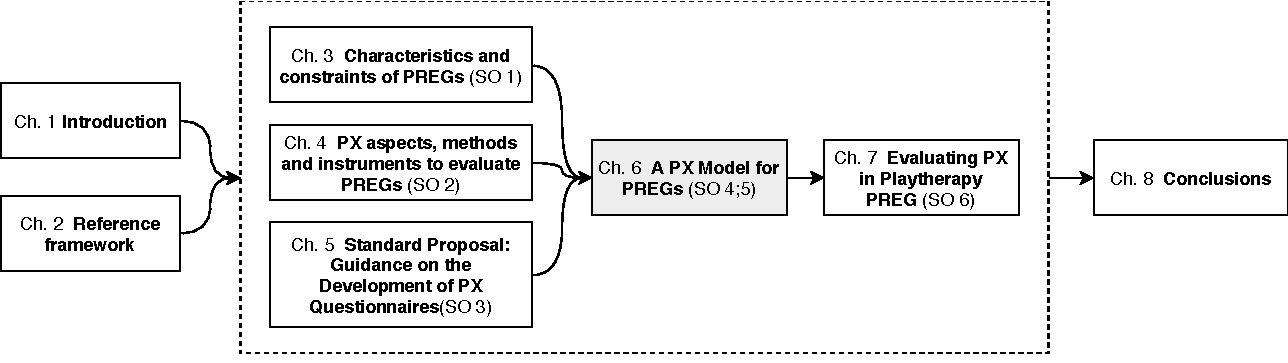
\includegraphics[width=\linewidth]{gfx/intro/documentOverview}} \quad
\caption{Overview of the document and relation between chapters (CH) and specific objectives (SO)}\label{fig:documentOverview}
\end{figure}

The remaining of the document is organised as follows: first, \autoref{ch:referenceFramework} presents the reference framework of the work and the state of the art of the \ac{PX} research field. After that, \autoref{ch:characterising} presents a qualitative study conducted to identify characteristics, constraints and an approach to characterise \acp{PREG} regarding \ac{PX}. Then, \autoref{ch:aspects} describes relevant aspects, methods and instruments to evaluate \ac{PX} in \acp{PREG} and the identification process that we carried out. After that, a comprehensive \ac{PX} model for evaluating \acp{PREG} is proposed in \autoref{ch:model}. Additionally, a methodology to evaluate \ac{PX} in \acp{PREG} based on the proposed model is presented in this section. Then, \autoref{ch:questionnaire} presents a standard proposal to develop \ac{PX} evaluation questionnaires and a questionnaire to assess physiotherapists' perception of \ac{PREG}. \autoref{ch:playtherapy} presents a case study in which the findings of this research work were employed to evaluate a \ac{PREG} developed by the Multimedia and Vision research group from \textit{Universidad del Valle} and Evaristo Garc\'ia University Hospital in Cali Colombia. Finally, we summarise and conclude the results of this research work in \autoref{ch:conclusions}.
\chapter{Reference Framework} % Chapter title
\label{ch:referenceFramework} % For referencing the chapter elsewhere, use \autoref{ch:examples} 

%----------------------------------------------------------------------------------------
%-------------------------------------------------------------------------
\section{Theoretical Framework}

\subsection{\ac{GUR} and \ac{PX}}
\label{subsec:gur}
According to \textcite{macklin2016games} a game is a work made to express, impart and provide experiences, producing play when interacting with it. \textcite{rogers2014level} defines a game as an activity that requires at least a player, has rules and a victory condition. \textcite{koster2013theory} states that a game is an iconic representation of real world patterns. \textcite{schell2015art} considers a game as a problem solving activity, which is approached with a playful attitude. Games create an imaginary world that absorbs players' full attention \autocite{michael:2006}. The main goal of games is to provide a fun and engaging experience to players \autocite{Moosajee,Zammitto2014}. Thus, evaluating the quality of the experience the games provide to players.

\ac{PX} is one of the most significant factors in determining the success of digital games in terms of aspects such as fun, flow, enjoyment, engagement, satisfaction, pleasure and playability. However, this concept is not used consistently in the literature \autocite{Wiemeyer2016} and sometimes is used interchangeably with other concepts such as playability, gamer experience, game experience or \ac{UX} \autocite{Bernhaupt2015}. For instance, in \autocite{Chu2011,GonzalezSanchez2009}, \ac{PX} is considered to be described by playability, while in \autocite{Nacke2009} playability is considered to be a prerequisite for a high quality of \ac{PX}. An accepted definition of \emph{\ac{PX}} is that it can be considered as an extension of \ac{UX} \autocite{Wiemeyer2016,GonzalezSanchez2009,Bernhaupt2015}. While, \ac{UX} represents the quality of interaction between users and software \autocite{Wiemeyer2016,Bernhaupt2015,Calvillo-Gamez2015}; while \ac{PX} denotes the personal experience of playing digital games, thus it involves subjective perceptions of players \autocite{Wiemeyer2016,Chu2011}. The goal of evaluating \ac{PX} is to improve interaction between players and games.

\ac{GUR} consists in the observation and analysis of \ac{PX} applying methods from different fields such as usability, psychology, play testing \autocite{Wiemeyer2016}, gameplay metrics \autocite{Drachen2013} and physiological evaluation \autocite{Nacke2015}. Thus, \ac{GUR} enables and fosters collaboration between \ac{PX} professionals, game developers and academic researchers \autocite{desurvire_methods_2013}. Below, \ac{GUR} methods and considerations when evaluating digital games are presented.

%Existing \ac{GUR} methods can be employed for evaluating \ac{PX}, however they may need adaptations for rehabilitation exergames since there are some issues which may alter \ac{PX} during interaction. These issues include: (i) exergames use non traditional interaction devices, such as movement sensors; (ii) players impairment may impose limitations to interaction, and (iii) intervention of other people (e.g. therapists) may be required \autocite{Wiemeyer2015,Nijholt2008}. Consequently, these issues should be considered when performing a \ac{PX} evaluation.

\subsection{\ac{GUR} Evaluation Aspects}
\label{subsec:aspects}

Selecting the aspects to be evaluated is a crucial task to be overcome when preparing an evaluation. However, selecting the most important aspects to evaluate is difficult \autocite{Nacked}. This selection depends on factors such as evaluation goal, available resources and development maturity of the evaluated game. There are different approaches to evaluate \ac{PX} in a general way, \textcite{Sanchez2009} presents an approach to evaluate \ac{PX} through playability; meanwhile, \textcite{Calvillo-Gamez2015} present a selection of aspects known as \emph{Core Elements of the Gaming Experience}, which are necessary but not sufficient for games to provide a positive experience.

Motivation and willingness to play can be evaluated in terms of other aspects such as immersion \autocite{Lapas2015,Nacke2009,VandenAbeele2016,Wiemeyer2016,Nijhar2012,Sanchez2009,Desurvire2009,Nijholt2008}, enjoyment \autocite{Ho2017,Li2016,VandenAbeele2016,Zhao2016,Li2006,Berkovsky2010}, challenge \autocite{Moosajee,Nacke2009,VandenAbeele2016,Wiemeyer2016,Desurvire2009}, flow \autocite{Lapas2015,Bernhaupt2015,Nacke2009,Wiemeyer2016,Nijholt2008}, presence \autocite{Lapas2015,Mader2012,Ho2017,Wiemeyer2016}, 
emotion \autocite{Bernhaupt2015,Sanchez2009,Wiemeyer2016}, engagement \autocite{Yanez-Gomez2017,Wiemeyer2016}, negative-positive affect \autocite{Nacke2009}, interest \autocite{VandenAbeele2016}, preference \autocite{Zhao2016}, autonomy \autocite{Wiemeyer2016,VandenAbeele2016} and 
absorption \autocite{Lapas2015}. Meanwhile, playability or usability, can be evaluated through aspects like satisfaction \autocite{Yanez-Gomez2017,Zhao2016,Sanchez2009}, ease of use \autocite{Moosajee,VandenAbeele2016,Cameirao2010}, learnability \autocite{GonzalezSanchez2009,Desurvire2009} and
acceptance \autocite{Yanez-Gomez2017}. Finally, game design can be evaluated using aspects including story \autocite{Moosajee,Desurvire2009}, clarity of goals \autocite{VandenAbeele2016,Desurvire2009}, tension, competence \autocite{Wiemeyer2016,Nacke2009}, camera \autocite{Moosajee},
game pace \autocite{Moosajee,Desurvire2009}, aesthetics, stimulation, identification \autocite{Bernhaupt2015}, audiovisual appeal, meaning \autocite{VandenAbeele2016}, involvement, curiosity, fantasy \autocite{Wiemeyer2016}, game adaptation \autocite{Wiemeyer2015,Ni2014,Cameirao2010,Nijholt2008} and social play \autocite{Wiemeyer2015,Sanchez2009,Yanez-Gomez2017,Lapas2015}.

However, as shown in \autoref{tab:aspects}, \ac{PX} aspects are categorised inconsistently within the literature. Aspects are categorised as properties, components, dimensions, constructs, facets, factors, areas or parameters.

\begin{table}[bht]
\caption{Categorisation inconsistencies for \ac{PX} evaluation aspects}
\label{tab:aspects}
\myfloatalign
\resizebox{0.8\linewidth}{!}{
\begin{tabular}{p{5.5em}lllllllllll}
\toprule
\multirow{2}{*}{\spacedlowsmallcaps{Aspect}} & \multicolumn{11}{c}{\spacedlowsmallcaps{Referred as}} \\
\cline{2-12}
&\rot{\small{\textit{Playability Aspect} \autocite{Yanez-Gomez2017}}}
&\rot{\small{\textit{Playability Property} \autocite{Sanchez2009}}}
&\rot{\small{\textit{GX Component} \autocite{Nijhar2012}}}
&\rot{\small{\textit{\ac{PX} Element} \autocite{Wiemeyer2016}}}
&\rot{\small{\textit{\ac{UX} Dimension} \autocite{Bernhaupt2015}}}
&\rot{\small{\textit{\ac{PX} Dimension} \autocite{Nacke2009}}}
&\rot{\small{\textit{\ac{PX} Component} \autocite{VandenAbeele2016}}}
&\rot{\small{\textit{\ac{UX} Facet} \autocite{Lapas2015}}}
&\rot{\small{\textit{Factor} \autocite{Ho2017}}}
&\rot{\small{\textit{Area} \autocite{Moosajee}}}
&\rot{\small{\textit{Gameplay Parameter} \autocite{Zhao2016}}} \\
\midrule
Immersion &  & X & X & X &  & X & X & X &  &  & \\
\midrule
Enjoyment &  &  &  &  &  &  & X &  & X &  & X \\
\midrule
Challenge &  &  &  & X &  & X & X &  &  & X & \\
\midrule
Flow &  &  &  & X & X & X &  & X &  &  & \\
\midrule
Presence &  &  &  & X &  &  &  & X &  &  & \\
\midrule
Social play & X & X &  & X &  &  &  & X &  &  & \\
\midrule
Satisfaction & X & X &  &  &  &  &  &  &  &  & X \\
\midrule
Feedback &  &  &  & X &  &  & X &  &  &  & \\
\midrule
Ease of use &  &  &  &  &  &  & X &  &  & X & \\
\midrule
Emotion &  & X &  & X & X &  &  &  &  &  & \\
\midrule
Engagement & X &  &  & X &  &  &  &  &  &  & \\
\midrule
\bottomrule
\end{tabular}}
\end{table}

\subsection{\ac{GUR} Evaluation Methods}
\label{subsec:methods}
The goal of applying \ac{GUR} methods is to determine whether a game offers a compelling and engaging experience to players \autocite{Yanez-Gomez2017,Bernhaupt2015}, collecting \ac{PX} data before, during and/or after players interact with the game (or game prototype) \autocite{Wiemeyer2016,Nacke2015,Mueller2015,Drachen2013}. Also, \ac{UX} and usability methods are commonly used for evaluating \ac{PX} \autocite{Yanez-Gomez2017,McAllister2015}. However, these are not sufficient for evaluating games, since standard metrics, such as task completion or error rates, do not map to metrics that may assess \ac{PX} properly. Therefore, traditional usability metrics should be used along with other forms of evaluation or should be extended \autocite{Wiemeyer2016,McAllister2015,Bernhaupt2015,Nackea,Hoysniemi2006}. \autoref{tab:methods} presents an overview of available \ac{GUR} methods for evaluating \ac{PX} grouped into five categories. Those categories are detailed below.

\begin{table}[bth]
\caption[\ac{GUR} methods for \ac{PX} evaluation]{\ac{GUR} methods for \ac{PX} evaluation}
\label{tab:methods}
\myfloatalign
\resizebox{0.86\linewidth}{!}{
\begin{tabular}{p{2.5cm}p{3.5cm}l}
\toprule
%----------------------
\spacedlowsmallcaps{Category} 
& \spacedlowsmallcaps{Description}
& \spacedlowsmallcaps{Method}
\\ \midrule
%----------------------
\multirow{12}{2.5cm}{User-oriented}
&
\multirow{12}{3.5cm}{Evaluation data is collected from players who represent the target audience}
&
Questionnaire \autocite{Yanez-Gomez2017,Ho2017,Wiemeyer2016,Nacke2015,Mueller2015,Zhao2016,Lapas2015,Nijhar2012,Nackea}
\\
&&
Interview \autocite{Wiemeyer2016,Moosajee,Nacke2015,Nijhar2012,Nackea}
\\
&&
Video recording \autocite{Wiemeyer2016,Moosajee,Mueller2015,Nijhar2012}
\\
&&
Field-Behavioural observation \autocite{Yanez-Gomez2017,Wiemeyer2016,Nacke2015}
\\
&&
Think-aloud protocol \autocite{Wiemeyer2016,Nacke2015,desurvire_methods_2013}
\\
&&
Focus groups \autocite{Yanez-Gomez2017,Nacke2015}
\\
&&
\ac{RITE} \autocite{Moosajee,Nackea}
\\
&&
Co-discovery learning \autocite{Yanez-Gomez2017}
\\
&&
Question-asking protocol \autocite{Yanez-Gomez2017}
\\
&&
Peer tutoring \autocite{Hoysniemi2003}
\\
&&
Prisoner dilemma task \autocite{Mueller2015}
\\
&&
Ethnography \autocite{Nackea}
\\\midrule
%----------------------
\multirow{4}{2.5cm}{Expert-oriented}
&
\multirow{4}{3.5cm}{A group of experts plays the role of players and inspect games}
&
Heuristic evaluation \autocite{Yanez-Gomez2017,Wiemeyer2016,Nacke2015,desurvire_methods_2013,Nackea,Nacke2009,Desurvire2009,Federoff2002}
\\
&&
Guidelines or standard inspections \autocite{Yanez-Gomez2017}
\\
&&
Cognitive walk through \autocite{Yanez-Gomez2017}
\\
&&
Pluralistic walk through \autocite{Yanez-Gomez2017}
\\\midrule
%----------------------
\multirow{3}{2.5cm}{Automated}
&
\multirow{3}{3.5cm}{Evaluation data is collected direct from games}
&
Gameplay metrics \autocite{Nacke2015,Nackea,Nacke2009}
\\
&&
Game logs \autocite{Wiemeyer2016}
\\
&&
A/B Testing \autocite{desurvire_methods_2013}
\\\midrule
%----------------------
\multirow{7}{2.5cm}{Physiological}
&
\multirow{7}{3.5cm}{Evaluation data is collected direct from players' body surface}
&
Biometrics analyse \autocite{Nacke2009}
\\
&&
\ac{EEG} \autocite{Wiemeyer2016,Nacke2015}
\\
&&
\ac{EMG} \autocite{Wiemeyer2016,Nacke2015}
\\
&&
\ac{EDA} \autocite{Wiemeyer2016,Nacke2015}
\\
&&
\ac{HR} \autocite{Wiemeyer2016,Nacke2015}
\\
&&
Body movement coding \autocite{Mueller2015,Nijhar2012}
\\
&&
Eye-tracking \autocite{Wiemeyer2016,Nackea}
\\\midrule
%----------------------
\multirow{3}{2.5cm}{Psychological}
&
\multirow{3}{3.5cm}{The collected data is used to model player and \ac{PX}}
&
Persona modelling \autocite{Wiemeyer2016,Nackea}
\\
&&
Player modelling \autocite{Wiemeyer2016,Nackea}
\\
&&
Cultural debugging \autocite{Nackea}
\\\midrule
%----------------------
\bottomrule
\end{tabular}}
\end{table}

\subsubsection{User-oriented}
User-oriented methods involve players during \ac{PX} evaluations to gather data such as behaviours, reactions, opinions, comments and suggestions \autocite{Yanez-Gomez2017,Bernhaupt2015,Drachen2013}. Frequently used methods include questionnaires \autocite{Yanez-Gomez2017,Ho2017,Wiemeyer2016,Nacke2015,Mueller2015,Bernhaupt2015,Zhao2016,Lapas2015,Nijhar2012,Nackea}, interviews \autocite{Wiemeyer2016,Moosajee,Nacke2015,Nijhar2012,Nackea}, video recording \autocite{Wiemeyer2016,Moosajee,Mueller2015,Nijhar2012}, field observation \autocite{Yanez-Gomez2017,Wiemeyer2016,Nacke2015}, think-aloud protocol \autocite{Wiemeyer2016,Nacke2015,desurvire_methods_2013}, focus groups \autocite{Yanez-Gomez2017,Nacke2015}, co-discovering learning \autocite{Yanez-Gomez2017}, question-asking protocol \autocite{Yanez-Gomez2017} and ethnography \autocite{Nackea}. Although, there are some standardised questionnaires and scales which can be used \autocite{denisova_convergence_2016,VandenAbeele2016,Calvillo-Gamez2015,Brockmyer2009,Poels2008,DeKort2007,Vorderer2004}, the use of ad-hoc questionnaires is the most preferred approach \autocite{Yanez-Gomez2017}. Some user-oriented methods, such as \ac{RITE} \autocite{Moosajee,Nackea}, have been developed in the game development context. Also, evaluators may need adapt or create methods to meet specific evaluation requirements. For instance, evaluators have employed peer tutoring for evaluating PX in exergames for children \autocite{Hoysniemi2003}; and prisoner dilemma task for evaluating players competitiveness and cooperation behaviours in an exergame \autocite{Mueller2015}.

User-oriented methods can be used along the whole development life-cycle based on the current needs and the availability of users to participate. If the number of available users is low, methods such as interviews, field observations, think-aloud protocol and co-discovery learning are convenient. In case of questionnaires, focus groups and \ac{RITE} evaluators should consider some issues. First, evaluators should plan well in advance if a high number of users is needed for a questionnaire evaluation. In such a case, they should plan a recruitment strategy. Similarly, evaluators should determine the number of sessions to be conducted when using focus groups. Finally, \ac{RITE} requires evaluators and developers to test and fix the evaluated game iteratively during an evaluation session. In that case, evaluators should adapt evaluation location to facilitate conditions for developers to fix identified issues.

\subsubsection{Expert-oriented}
In this case, a group of experts inspect a game to identify possible issues which may affect PX \autocite{Bernhaupt2015,Yanez-Gomez2017}. There are two common approaches when applying expert-oriented methods: experts assess whether a game meets a set of principles; i.e., heuristics \autocite{Yanez-Gomez2017,Wiemeyer2016,Nacke2015,desurvire_methods_2013,Nackea,Nacke2009,Desurvire2009,Federoff2002}, guidelines or standards \autocite{Yanez-Gomez2017}; and experts play the role of a player performing a set of typical tasks, using cognitive and/or pluralistic walk-through \autocite{Yanez-Gomez2017}.

The most used expert-oriented methods are heuristic evaluation \autocite{Desurvire2009,Federoff2002,Hochleitner2015,Tondello2016} and guidelines inspection \autocite{Yanez-Gomez2017}, which are convenient for evaluating games when players are not available. In the case of exergames, there are some guidelines \autocite{Wiemeyer2015,Pasch2009,Isbister2015,Mueller2014} that evaluators can use. Expert-oriented methods are appropriate for performing PX evaluations during early stages of game development \autocite{Bernhaupt2015,McAllister2015,desurvire_methods_2013}. However, results of these methods depend directly on evaluators’ expertise. 

\subsubsection{Automated}
Automated methods allow collecting \ac{PX} data from games using programmed hooks \autocite{Nacke2015}. The collected data will be used to get information about players behaviour during interaction. Automated evaluation methods are considered objective since they allow collecting quantitative data. Additionally, automated methods can be useful for performing A/B testing, which is used to compare several versions of a game and decide over different design alternatives \autocite{desurvire_methods_2013}. The most common automated methods are game-play metrics \autocite{Nacke2015} and game logs \autocite{Drachen2013,Wiemeyer2016}.

\subsubsection{Physiological}
These methods allow collecting player’s body signals, which are used to understand the experience that players have while interacting with a game \autocite{Wiemeyer2016,Nacke2015}. Evaluators can use these methods to monitor internal body reactions before, during and after interaction \autocite{Mueller2011}. Physiological methods include eye-tracking \autocite{Wiemeyer2016,Nackea}, \ac{EDA} \autocite{Wiemeyer2016,Nacke2015}, \ac{EMG} \autocite{Wiemeyer2016,Nacke2015}, \ac{EEG} \autocite{Wiemeyer2016,Nacke2015} and \ac{HR} \autocite{Wiemeyer2016,Nacke2015}. Like automated, physiological methods are objective. Also, biometric analyse \autocite{Nacke2009} or body movement coding \autocite{Mueller2015,Nijhar2012} can be used to analyse the data collected during an evaluation. In case of exergames, evaluators should be careful when using \ac{EDA}, \ac{EMG} or \ac{EEG} measurement since patient’s movements could be limited by data collection instruments, which is a difficulty if an exergame requires movements like shifts or squats.

\subsubsection{Psychological}
Psychological methods are useful for collecting data about cognitive, perceptual and emotional experiences \autocite{Wiemeyer2016,Nackea}. Those data are relevant since perceived experience is a personal and subjective perception. A well-known psychological method is Persona modelling \autocite{Wiemeyer2016,Nackea}, which allows representing and understanding players mental model. Player modelling is a method used to adapt PX according to players behaviour during gameplay \autocite{Wiemeyer2016,Nackea}. Cultural debugging is used to determine cultural differences that may affect PX \autocite{Nackea}. Psychological methods are useful to identify target users who can participate in evaluations.

%\subsubsection{Evaluation Methods for Rehabilitation Exergames}

%In the case of rehabilitation exergames, all the above mentioned methods can be employed to evaluate \ac{PX}. However, some issues that may affect \ac{PX} and rehabilitation process should be considered. These issues include: 

%\begin{itemize}
    %\item Evaluation should not only focus on fun, but also on the health goal that is being pursued by a game \autocite{Iacovides2015}.
    %\item Game should adapt to particular player's needs \autocite{Wiemeyer2015,Ni2014,Cameirao2010,Nijholt2008}.
    %\item Player modelling should consider target audience's health conditions \autocite{Mader2012,Wiemeyer2015}.
    %\item Cheating the rehabilitation goal of a game should be avoided \autocite{Ni2014}.
    %\item Player distractions should be avoided \autocite{Ni2014}.
    %\item Family members and clinicians should be included since they may intervene during interaction \autocite{Wiemeyer2015}.
    %\item Game feedback should be evaluated, since it has to be positive \autocite{Wiemeyer2015}.
%\end{itemize}

In the case of digital games used in physical rehabilitation, there is no a defined approach to evaluate \ac{PX}. Some authors state that methods have to be selected, adapted and/or combined depending on the particular case being evaluated \autocite{Yanez-Gomez2017,Wiemeyer2016,Mueller2015}. Additionally, an objective evaluation may be achieved collecting qualitative and quantitative data. That is known as mixed or multi-method approach \autocite{Nacke2009,Iacovides2015,Drachen2013,Mueller2015,Zammitto2014}.

\subsection{\ac{GUR} Evaluation Instruments}
\label{subsec:instruments}
The selection of tools to be used while evaluating \ac{PX} depends on the methods, aspects and game involved in the evaluation. Evaluators can use different standardised questionnaires to evaluate PX depending on the aspects to be evaluated.

The \textit{PX inventory} \autocite{VandenAbeele2016} is a scale based on the \ac{MDA} framework and evaluates eleven aspects of \ac{PX} including enjoyment, mastery, ease of control, progress feedback and audio-visual appeal. It groups the aspects into three levels: value, functional and psycho-social, and each level is evaluated using a sub-scale. The inventory was developed along two iterations, involving a group of experts and based on other 124 existing scales. 

\textit{\ac{CEGEQ}} \autocite{Calvillo-Gamez2015} is composed of 38 items and was developed involving game reviews and interviews with a game designer, two game reviewers and one player. The aspects evaluated by this questionnaire include: enjoyment, scenario, rules, ownership and control.

The \textit{\ac{GEQ}} is a modular questionnaire composed of a core questionnaire, a post-game questionnaire and social presence questionnaire \autocite{Poels2008}. This questionnaire was developed during focus groups and expert meetings considering existing questionnaires. Seven aspects are evaluated by the core questionnaire: sensory and imaginative immersion, tension, competence, flow, negative affect, positive affect and challenge.

The \textit{\ac{GEQ2}} \autocite{Brockmyer2009} is composed of 19 items and evaluate four aspects: absorption, flow, presence and immersion. It was developed along three iterations.

The \textit{EGameFlow Scale} \autocite{Fu2009} is composed of 42 items and allow evaluating concentration, goal clarity, feedback, challenge, autonomy, immersion, social interaction and knowledge improvement. This scale is intended to evaluate e-learning games; thus, an adaptation for evaluating other kinds of games may be required.

Furthermore, evaluators can use questionnaires for evaluating specific aspects. An immersion questionnaire is presented in \autocite{jennett2008measuring}, it allows evaluating immersion quantitatively based on basic attention, temporal dissociation, transportation, challenge, emotional involvement and enjoyment. Also, the \ac{SPGQ} \autocite{DeKort2007} evaluates social presence in terms of empathy, negative feelings and behavioural involvement. It was developed based on focus groups, interviews and another social presence scale. Additionally, \ac{UX} scales \autocite{Brooke1996} and questionnaires \autocite{Laugwitz2008,Hassenzahl2003,lund2001measuring} can be employed to evaluate aspects such as usability, ease of use and satisfaction.

With reference to expert-oriented methods, the heuristics presented in \autocite{Desurvire2009,Federoff2002,Tondello2016} can be employed for initial evaluations of game design. Similarly, there are design guidelines \autocite{Wiemeyer2015,Isbister2015,Mueller2014} and principles \autocite{Berkovsky2010} specialised for exergames. Regarding physiological methods, biometric storyboards \autocite{Mirza-Babaei2014} are appropriate to visualise, relate and analyse collected data; e.g., player's physiological data, self-reported events and in-game events.

Additionally, evaluators can use models to assess and validate PX evaluation results. Some models include: the motivation model for exertion games \autocite{Li2016}, which is based on the \ac{SCT} and relates a game avatar with \ac{PX} in exergames. This model suggests that self-presence is positively associated with identification, which is also positively associated with enjoyment. Moreover, the presence, enjoyment and mood experience model \autocite{Ho2017} relates subjective level of presence, game enjoyment and mood experience to players' attitude towards exertion games. Furthermore, the model presented in \autocite{Mader2012} allows describing and analysing the relation among a player, a game and a therapy. This model assists in deciding which information should be collected, examining game design coherence and identifying constraints imposed by a therapy. Moreover, models such as the \ac{4LM} \autocite{Mueller2011}, the \ac{ISCAL} \autocite{Zhang2011} and the Dual Flow Model \autocite{Sinclair2007} may be useful to select which aspects are relevant to evaluate exergames.

Finally, \textcite{Ni2014} presents a design and evaluation framework for virtual rehabilitation based therapy games. The framework was developed with the active participation of a group of children and therapists. The authors present a list of design requirements for virtual rehabilitation based therapy games and characteristics of a game for health. \textcite{kendzierski1991physical} describe the physical activity enjoyment scale, which can be used to evaluate enjoyment in virtual rehabilitation based therapy games.

%----------------------------------------------------------------------------------------

\section{State of the Art}
\label{sec:px_ux_models}

To the extent of author's knowledge a \ac{PX} evaluation model for \acp{PREG} is not defined yet. However, some \ac{PX} models for general or specific purposes are presented below.

%----------------------
\subsection{The \ac{IMP}} 
% three elements: context,player and game
% time: pre-game, game, post-game

\textcite{Elson2014} present the \ac{IMP} which is an integrative model intended to be used for game user research purposes and is based on other literature. According to this model, \ac{PX} is comprised by three elements: player, i.e., (players' traits and states); game, i.e., the media and game characteristics and context, i.e. the setting and the social environment. The model claims that those three elements are affected along three consecutive phases. The model is illustrated in \autoref{fig:IMP_Model} and described below.

First, the Pregame phase corresponds to anything that occurs before playing a game. This phase results in the players' decision of playing or not a game. In this phase, the Context element is defined by cultural parameters that affect the player's selection of games. Context is characterised by some factors including cultural norms, marketing, social acceptance, peer groups and family. Meanwhile, the Player element is defined the characteristics of players as individuals, which includes biologic and demographic variables. Finally, the Game element is defined by its current availability and marketing attraction factors.

Second, the Game phase corresponds to the actual situation of playing or using a game. Context in this phase is determined by experimental aspects such as employed devices, location, platforms and the presence of other players. The Player element comprises the sum of psychological processes and behaviours including game enjoyment, presence and flow. The game element refers to the content and mechanisms of the game being played.

Third, the Post-Game phase includes the post-use effects of a singular or repeated episodes of game playing. The Post-Game forms a feedback loop that can affect the next gaming episode. In this phase, the Context element comprises all forms of communication caused or inspired by playing a game. The Player element is defined by internal states and behaviours of players after interacting with a game, which may be undesired. The effects on players can be short-term, i.e., temporary changes in thoughts, feelings and behaviours; or long-term, i.e., consequences of repeated episodes of game playing. The model does not describes the Game element in this phase.

\begin{figure}[bth]
\myfloatalign
{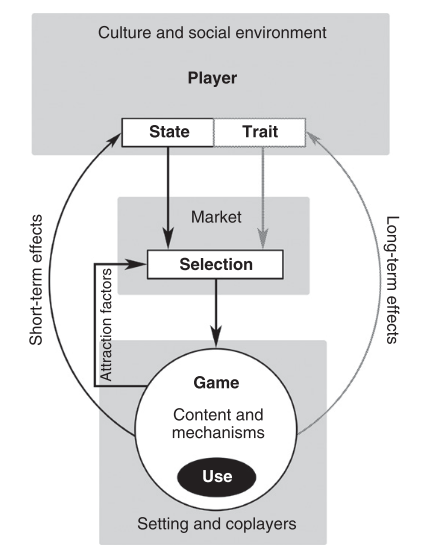
\includegraphics[width=.6\linewidth]{gfx/ref_framework/IMP_Model}} \quad
\caption[The \ac{IMP}]{The \ac{IMP} \autocite{Elson2014}}\label{fig:IMP_Model}
\end{figure}

%----------------------
\subsection{The Contextual Gameplay Experience Model}
\textcite{Engl2013} present the Contextual Gameplay Experience Model based on the ideas presented in \autocite{Nackea2,Nacked}. It was built to study the gameplay experience in mobile games focusing on contextual influences that may affect it. Before a main study the authors conducted two pre-studies. First, an online survey was carried out to ask about mobile game contexts and motivations to play mobile games. They identified two main contexts; i.e., mobile and home. Second, they used the interview and observation methods with sixteen participants to study both contexts. They found that the main motivation to play mobile games is to kill time.

They employed interviews and video recording for the main study and involved thirty five participants. They selected two games to be played by participants and used \ac{GEQ} to evaluate experience in a public transportation setting (mobile) and a home setting. They found that the participants had a more immersive experience in the mobile setting, though they felt stronger negatively affected that in the home setting. Additionally, they identified that the experience can by affected by spatial, temporal. social, cultural and psychological influences.

Based on their findings, the authors proposed a model based on three layers of abstraction. The most concrete layer is the game system, which represents the game itself and the gaming device. This layer is mainly functional and corresponds to the playability of the game. The second layer is the player, which comprises the internal influences and characteristics of players. It represents the individual experience of a player, which results from the interaction between him/her and a game. The most abstract layer corresponds to the external influences that affect the contextual gameplay experience. The model is illustrated in \autoref{fig:context_gp_exp}.

\begin{figure}[bth]
\myfloatalign
{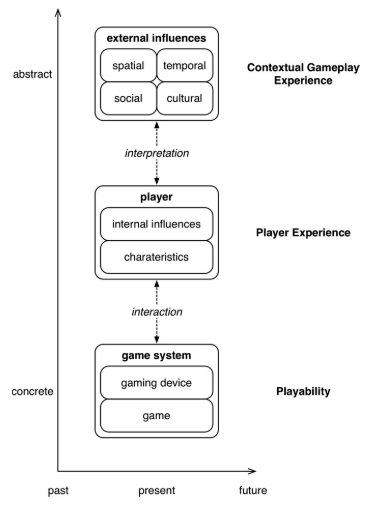
\includegraphics[width=.6\linewidth]{gfx/ref_framework/context_gp_exp}} \quad
\caption[The Contextual Gameplay Experience Model]{The Contextual Gameplay Experience Model \autocite{Engl2013}}\label{fig:context_gp_exp}
\end{figure}

%----------------------
\subsection{Playability}
\label{sec:playability}
\subsection{A Physiological Evaluation Model for Flow-Experience in VR Games: Construction and Preliminary Test}

\textcite{Bian2015} present a physiological model for evaluating flow experience in virtual reality games. Flow is a state in which players are fully immersed and engaged in a game.

Flow is mainly evaluated using self-report questionnaires, which collect data from players after interaction. This evaluation have two main limitations: (i) collected evaluation data is subjective and (ii) data collection occurs when players are not in flow state anymore.

The proposed model addresses these two issues using physiological flow indicators which are measured during interaction. The model includes 5 first level indicators, which are: \ac{EMG}, cardiovascular activity, \ac{EDA}, respiratory activity and \ac{EEG}.

After conducting an empirical study, obtained results revealed that heart rate, inter beat interval, heart rate variability, low-frequency band, high frequency band heart rate variability, and respiratory rate predict flow experience effectively.

%----------------------
\subsection{User Satisfaction Evaluation Model Based on Blink Interval}

\textcite{hou2015} present a user satisfaction evaluation model based on blink interval. The model is intended to overcome weaknesses of usability methods like self-report questionnaires providing and objective evaluation model. These weaknesses include: users tend to choose what is socially desirable, they may get confused about definitions of scales and they may get bored when answering long questionnaires, consequently the tend to provide random answers.

The authors found that blink interval may a be an effective physiological indicator of user satisfaction. They identified a strong correlation between user's blink interval and their satisfaction when using a system. The results showed that the lower the satisfaction is, the longer the blink interval is. To validate the model an eye tracker was employed. 31 participants were asked to perform two tasks: shop online and tag on a micro blog.

The limitations of the model are related to the impact that environment could have on blink interval. Also, authors remark that the model would be more appropriate for identifying user dissatisfaction.


\chapter{Characteristics and constraints of \acp{PREG}}
\label{ch:characterising}

To develop a \ac{PX} evaluation model for \acp{PREG}, we should understand what a \ac{PREG} represents and how to characterise it for evaluation purposes considering its therapeutic purpose. In this section, we propose a definition of \acp{PREG} considering that those are exergames, have therapeutic purposes and are used within rehabilitation therapies. Then, we present a set of constraints to consider when evaluating \acp{PREG}. Finally, we propose an approach to characterise \acp{PREG} for evaluation purposes based on the proposed definition and constraints.

%-----------------------------------
\section{Defining \acp{PREG}} % Definition --------------------------
\label{sec:def_reh_ex}
\acp{PREG} should be defined considering their nature as exergames, their therapeutic purposes and their use as part of rehabilitation therapies. Below, we study those three aspects and propose a definition for \acp{PREG}.

\subsection{Exergames}
\label{sub:def_ex}
% Definition
According to \textcite{Mueller2011}, an exergame is a game that employs body movement to enable player's interaction; i.e., the outcome of the game is determined by the player's physical effort. Also, \textcite{Pirovano2016} defines an exergame as a game built into an exercise structure. This definition implies that the associated exercises should guide the whole game design process. It may be important for \acp{PREG} since exercises are directly related to their therapeutic purpose. Furthermore, \textcite{Sinclair2009}, defines an exergame as a merger of a digital game with exercise equipment, emphasising the role that the interaction devices play in the experience of playing exergames.

\subsubsection{Exergames Models}
\label{subsub:eg_models}
Exergame models allow achieving a comprehensive understanding of what the exergame concept may comprise. Below, we outline three of these models:

\begin{enumerate}
    \item \emph{The Four Lenses Model}: \textcite{Mueller2011} propose an exertion framework as an attempt to describe how exergames can use technology to create more compelling exergames. This framework is based on the four lenses, as they call them, and is centred on the player's body to understand the interaction. The four lenses allow considering the body in a structured way when designing an exergame.
    
    The first lens is \emph{The Responding Body}, which concerns with the internal body reactions before, during and after physical activity. The responding body impacts the design process since it affects interaction; i.e., when a player becomes fatigued or stronger as a consequence of exercise. Thus, the game challenge should adapt to player needs and skills, by controlling or monitoring responding body using physiological methods such as \ac{HR} or \ac{EEG}.
    
    The second lens is \emph{The Moving Body}, which corresponds to the re-positioning of the player's body parts during physical activity. Intensity, continuity and variety of the movement can enrich the game experience by providing resources and constraints to the exercise involved in a game.
    
    The third lens is \emph{The Sensing Body}, which describes how the player's body senses and experiences the world, including physical and virtual objects involved in a game exercise. Considering the sensing body during design may allow designers to achieve a richer game experience in a hybrid space
    
    The fourth lens is \emph{The Relating Body}, which encompasses how players relate to other people and technology. Adding a social layer to a game is key for people to participate in physical activity.
    
    Additionally, \textcite{Mueller2011} highlight some characteristics of exergames. First, uncertainty is desirable since it contributes to offering suspense and surprise along the experience. Particularly, game designers should consider that player's exercising brings a degree of uncertainty since his/her body movements are unpredictable. Thus, they should manage the relationship between the programmed uncertainty and the uncertainty arising from the player's exercise. Second, movement awareness contributes to \ac{PX} when exercising. Increasing movement awareness of players; e.g., by providing feedback about energy expenditure; may foster competition among them. While decreasing such awareness will distract the player from discomfort caused by exercising. Third, the player's expression of exertion may arise naturally as in sports. Although such expression does not allow a player to progress along the game, it contributes positively towards \ac{PX}. An exergame may support expression by highlighting players responding body characteristics. Fourth, adding rhythm to the game exertion can benefit aspects such as motor skills acquisition and discomfort dissociation. Fifth, designers should consider that exertion has an associated risk of injuring players in order to avoid a negative \ac{PX}. Finally, exergames have to assist players in understanding the associated exertion. It will enable players to play consciously and safety; e.g., knowing \ac{HR} while jogging allows a player to plan future activity. By mapping physical movements to a virtual world meaningfully is key to support exertion knowledge.
    
    \item \emph{\ac{ISCAL} Model}: \textcite{Zhang2011} proposed this model to build a Virtual Network Marathon. The model is based on five constructs: immersion, scientificalness, competitiveness, adaptability and learning. Immersion is the subjective impression of participating in a "realistic" exercise experience. Meanwhile, scientificalness means to perform exercise effectively and to avoid over-exercise; e.g., by including warming up and cool down stages before and after the exercise. Moreover, competitiveness enables players to satisfy their need of “getting better” at something. Adaptability refers to adjusting the game difficulty dynamically according to each player's needs. Finally, learning refers to offering players the opportunity to learn something while participating in the physical activity. \citeauthor{Zhang2011} argue that an exergame should support all constructs in order to provide an engaging experience.
    
    \item \emph{Dual Flow Model}: \textcite{Sinclair2007} propose this model due to the two purposes of an exergame: exercising and entertaining. The model comprises two constructs: attractiveness and effectiveness. Attractiveness motivates players to play and to continue playing in the future. It is closely related to fun and may be achieved by offering a balance between game challenges and player skills. That is, maintaining players in the flow zone \autocite{flow}.
    Effectiveness relates to the exercise involved in a game. An effective exergame has to result in health benefits for players, including fitness or rehabilitation. \citeauthor{Sinclair2007} propose a flow zone associated with the exercise involved in the game. In this case, an exergame has to provide a balance between the intensity of the exercise and the player's skills to perform the said exercise. A physiologically imbalanced exergame results in failure, deterioration or no-benefit for players. To achieve balance, an exergame has to collect feedback form player about fatigue, exercise level and boredom to adjust the challenge level accordingly.
\end{enumerate}

\subsection{Therapeutic games}
\label{sub:def_therapeutic_g}
A therapeutic game provides a cognitive or motor training to improve patient's health condition \autocite{Mader2012}. Specifically, a therapeutic exergame has to support the primary and secondary goals of exercises. Primary goals correspond to the movements involved in an exergame. Those are achieved by mapping desired movements into gameplay mechanics. Meanwhile, secondary goals refer to the correctness with which patients perform the expected physical exercises \autocite{Pirovano2016}. Thus, secondary goals differentiate therapeutic exergames form normal exergames, and movement correctness should be ensured when using exergames for therapeutic purposes.

\subsection{Rehabilitation therapy}
\label{sub:def_rehab_therapy}
Rehabilitation aims to enable people with disabilities to participate in daily life activities by improving their health status \autocite{Wiemeyer2015}. To regain lost functions, patients must execute repetitive movements correctly \autocite{PirovanoAdvisor2012}. A typical therapy session includes the following tasks and activities:

\begin{enumerate}
    \item \emph{Configuration and Personalisation}: physiotherapists select correct exercises, establish therapy goals according to patients’ initial diagnosis and schedule therapy sessions.
    \item \emph{Supervision}: includes \textit{monitoring} correct execution of movements, \textit{providing immediate feedback} to guide patients along therapy sessions, \textit{adapting} patient’s movements and postures according to his/her performance, \textit{extracting physiological and motion data} and \textit{motivating} patients to complete their therapy.
    \item \emph{Assessment}: physiotherapists should use gathered to \textit{assess} obtained results and \textit{adapt} therapies according to patient’s progress.
\end{enumerate}

Therefore, we define a \ac{PREG} as follows:\\

\emph{A \ac{PREG} is a therapeutic exergame that assists rehabilitation therapies in one or more tasks.}

%-----------------------------------
\section{Materials and methods} % Materials -----------------------------------
\label{sec:mats_mets_char}
% Interviews (Include leading questions), observation, (/)
% Thematic content analysis (for qualitative research) using affinity charts (/)
% One coder (/)
% Validation: Review by physiotherapists (/)
\subsection{Participants}
We conducted five semi-structured interviews along two sessions. Two physiotherapists participated in both sessions, while a third physiotherapist joined the second session. All physiotherapists belong to the Evaristo Garc\'ia University Hospital in Cali Colombia. The goal of the first session was to characterise the context in which \acp{PREG} are employed. We aimed to identify possible constraints that might limit the evaluation of \ac{PX} for this kind of games. We guided the interview of the first session using the following questions:

\begin{enumerate}
    \item What kind of patients participate in physical therapies?
    \item How is the patients' motivation towards physical therapies?
    \item What factors affect patients' motivation towards physical therapies?
    \item What activities occur during physical therapy sessions?
    \item Who participates in physical therapy sessions?
    \item How long does a therapy session takes?
    \item What information is collected during therapy sessions?
    \item How is patients' progress tracked?
\end{enumerate}

The goal of the second session of interviews was to identify physiotherapists expectations and requirements regarding the use of \acp{PREG}. One of the physiotherapists had been collaborating in the development of a collection of \acp{PREG}. The second interviews were conducted using the following questions.

\begin{enumerate}
    \item Who can decide if a patient can use a \ac{PREG} as part of his/her therapies?
    \item How can a \ac{PREG} be used as part of a physical therapy?
    \item When can a \ac{PREG} be used as part of a physical therapy?
    \item How do you expect to use \acp{PREG}?
    \item How do you expect that \acp{PREG} assist patients?
\end{enumerate}

Both interviews were recorded. We analysed the collected data using the thematic content analysis method \autocite{Burnard2008}. We transcribed all interviews to produce a list of relevant statements. The selected statements were closely related to one or more of the mentioned questions. Then, we assigned a theme to each statement to produce our initial coding framework. After that, we grouped themes to reduce the number of categories. We continued until we obtained four categories for our final coding framework. The final coding framework was shared with one of the physiotherapists to validate that our results represented participants views. The physiotherapist clarified or added information to five statements, this validation did not affect the resulting categories. The conducted study is illustrated in \autoref{fig:constraintsIdentification}.

\begin{figure}[htb]
\myfloatalign
{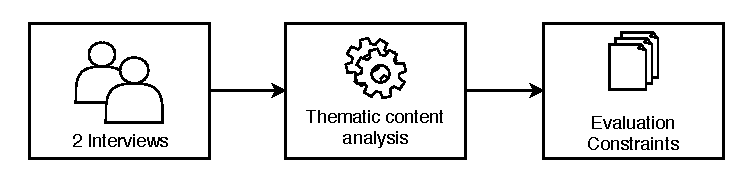
\includegraphics[width=\linewidth]{gfx/characterisation/constraintsIdentification}} \quad
\caption{Evaluation constraints identification process}\label{fig:constraintsIdentification}
\end{figure}

%-----------------------------------
\section{Findings} % Findings -----------------------------------
\label{sec:findings_char}
%-----------------------------------
\subsection{Constraints of evaluating PX in \acp{PREG}} % Constraints -----------------------------------
\label{sec:constraints}

\acp{PREG} have constraints that evaluators should consider to perform a relevant PX evaluation. Otherwise, the occurrence or completion of such evaluation may be affected. After transcribing interviews, we identified 57 statements regarding possible constraints of \acp{PREG}. After grouping and categorising the statements iteratively, we identified 4 final categories: patient condition (30 statements), rehabilitation context (18 statements), rehabilitation goal (7 statements) and interaction devices (2 statements). The statements regarding the first and second category were repetitive or refer to very similar things.

After analysing the statements and categories. We found that rehabilitation constraints are directly related to the therapeutic purpose of \acp{PREG}. That is, these are related to the rehabilitation environment and goals, the limitations imposed by players' impairments and the use of non-traditional interaction devices. Moreover, each \ac{PREG} may have additional constraints derived from its context of use, which evaluators should identify when planning a \ac{PX} evaluation.

\subsubsection{Rehabilitation goal constraints}
\label{sec:reh_goal_constraints}
The effectiveness of a \ac{PREG} has to be evaluated according to its impact on a rehabilitation therapy, i.e., assisting in the achievement of the associated rehabilitation goal and motivating patients towards their therapies. Such evaluation may require clinical tests and instruments and physiotherapists participation. Thus, evaluators should concentrate on aspects associated with movement execution such as amplitude, accuracy or speed to assess rehabilitation goal achievement. Also, they should evaluate aspects like enjoyment or engagement to asses motivation. Those evaluations may occur along the whole development life cycle.

In early development stages, evaluators should concentrate on evaluating if the evaluated \ac{PREG} meets the requirements to achieve its goal when used as part of a therapy. They may assess if the design process is focused on a rehabilitation goal; i.e., if the game mechanics relate directly to a set of movements and the exercises can be configured to personalise the experience according to patients' needs. They must evaluate if the \ac{PREG} can be used by patients safely, assessing aspects such as movement mapping correctness, adaptation capability and configuration capability and correctness. 

Moreover, they should assess the quality of the feedback provided by the exergame. It may give information about rehabilitation progress and exercise correctness. Additionally, evaluators should assure that the \ac{PREG} is playable during the time required by physiotherapists; e.g., 5 to 10 minutes for warming up, 20 for stimulus and 5 for cooling down. Finally, the \ac{PREG}, or an accompanying system, should offer quantitative data about patients overall progress including movement accuracy, success rate, allowing physiotherapists to make decisions based on rehabilitation goal achievement.

\subsubsection{Rehabilitation context constraints}
\label{sec:reh_context_constraints}
Evaluators should include patients and physiotherapists to evaluate a \ac{PREG} integrally. Such inclusion may be regulated or limited by constraints imposed by the rehabilitation context. First, patients' opportunity to use a \ac{PREG} on their therapies depend on physiotherapists' criteria. Thus, \acp{PREG} would meet physiotherapists' needs and expectations. They want those games to facilitate their job, thereby being a supporting tool that do not increase the amount of work load that they already have. That is, \acp{PREG} should be useful and practical for physiotherapists. Second, the supervision of physiotherapists is required to assure patients safety. Evaluators should consider that physiotherapists’ participation may alter interaction. Third, if the exergame is designed to be used in a health institution, some evaluations should occur there to assess the exergame in the real context. Therefore, evaluation logistics, such as time, number of participants, duration and location, usually will depend on them. Thus, evaluators should plan evaluation sessions considering internal regulations of the involved institution. Finally, although paper-work imposed by the health institutions does not relates directly with \ac{PX}, it can affect patient's motivation to even start a therapy.

\subsubsection{Patients' condition constraints}
\label{sec:reh_patients_constraints}
\acp{PREG} are targeted at people who need to recover lost functions. Therefore, evaluators should clearly define who can participate during evaluations. They should define the participants' physiological and therapeutic characteristics. Modelling Personas would be an appropriate approach to achieve such definition \autocite{Mader2012}. After that, an important aspect to evaluate is the capability of an exergame to be configurable to meet particular characteristics of target patients. The exergame should be safe for patients. Thus, initial evaluations should involve healthy subjects, e.g. physiotherapists, as stated by \textcite{Chu2011}.

With regards to patients' performance, exercises execution correctness must be assured, while fatigue and over-exercise must be avoided as stated by other authors \autocite{Pasch2009,Isbister2015,Zhang2011}. If the evaluated \ac{PREG} does not perform those tasks automatically, it may facilitate physiotherapists supervision; e.g., by allowing to pause and reconfigure game sessions.

Additionally, patients' expectations about their therapies are related to its daily life. Their main expectation is to complete their treatments as soon as possible to return to their daily life routines. Sometimes, they feel more motivated when therapies are challenging since they consider that the recovery process will be effective and fast. Therefore, physiotherapists should balance treatments to meet those expectations without compromising patients' health status. In that context, if patients believe that a \ac{PREG} does not contribute to their early recovery, they may not want to play them.

\subsubsection{Interaction devices constraints}
\label{sec:interation_dev_constraints}
\acp{PREG} use non-traditional interaction devices such as camera motion sensors. Input and output devices should allow patients to have a clear understanding of the outcome of their actions. For instance, a third person view is more appropriate than a first-person view, and big screens are preferred if patients should locate at a certain distance from the devices. Moreover, input devices should be natural and easy to use for patients. Those devices should allow making a meaningful mapping of rehabilitation movements and exercises. Finally, physical therapies include the use physical agents and objects that may affect what interaction devices can track.

%-----------------------------------------------
\subsection{Characterising a \ac{PREG}} % Characterising approach ----------------------------------
\label{sec:characterising}

To characterise a \ac{PREG}, we need a set of properties to understand its role within physical therapies. Such characterisation may be useful to define the scope of a PX evaluation. For instance, when evaluating an autonomous \ac{PREG}, aspects such as exercise monitoring and correction are highly important; however, if the \ac{PREG} only assists in motivating patients, those aspects would be irrelevant. We selected thirteen properties for characterising a \ac{PREG}. The first eight properties are based on the work presented in \autocite{PirovanoAdvisor2012}, and the remaining were defined according to the results of our study. We asked a group of physiotherapists to identify characteristics of \acp{PREG} that they consider relevant for evaluation purposes. Below, we describe the properties:

\begin{enumerate}
    \item \emph{Rehabilitation type}: \acp{PREG} can be \textit{wide-focused} if the game interaction requires patients whole body motion; or \textit{tight-focused} if the game interaction is enabled by a specific body part or a specific movement. Wide-focused \acp{PREG} are generally directed to upper and lower limbs and might require more space than wide-focused ones.
    
    \item \emph{Assisted tasks}: a therapy involves different tasks which can be assisted by \acp{PREG}. These tasks include configuration and personalisation, monitoring, feedback provision, adaptation, data extraction, motivation and assessment.
    
    \item \emph{Degree of autonomy}: this property is closely related to the supervision task of physical therapies. A \ac{PREG} can have one of 5 degrees of autonomy (See \autoref{tab:autonomy_dgree}). \textit{First-degree} \acp{PREG} support only motivation and require a physiotherapist to perform constant supervision. \textit{Second-degree} \acp{PREG} include adaptation features or constraint patient motion using robotic devices. This degree still requires constant physio-therapist supervision. \textit{Third-degree} \acp{PREG} require asynchronous physiotherapist supervision remotely or along periodic meetings. \textit{Fourth-degree} \acp{PREG} do not require physiotherapist supervision and could be considered standalone applications. However, certain input from physiotherapists is required; e.g., during diagnosis and assessment. \textit{Fifth-degree} are standalone \acp{PREG} that do not require any input from physiotherapists. Thus, all therapy tasks are performed using \ac{AI}. Fifth-degree is Utopian since current \acp{PREG} cannot replace physiotherapists labour.
    
    \item \emph{Configuration and assessment capability}: this property indicates whether a \ac{PREG} is \textit{closed-loop}, i.e., it can be configured and allows assessing patients performance; or \textit{open-loop}, i.e., it can be configured, but does not allow assessing patients performance.
    
    \item \emph{Input/output interaction devices}: A \ac{PREG} may include five types of input devices: \textit{standard, robotic, haptic, motion-enabled and camera-tracking}. Standard devices are traditional ones such as the mouse, keyboard, joystick and touch input. Robotic devices help patients perform correct movements. However, these devices may be expensive and invasive. Haptic devices provide some benefits of robotic devices at lower costs. Motion-enabled devices track users motion using accelerometers, gyroscopes or pressure sensors. Camera tracking devices allow body-free interaction, but they have some drawbacks associated with light conditions and tracking precision.
    
    Output devices include standard video and audio devices, joysticks with light or vibration feedback or novel devices supporting augmented, virtual or mixed reality.
    
    \item \emph{Thematic content}: indicates the content associated with a \ac{PREG}. It can be related to \textit{daily life activities}, e.g., cooking or walking. Also, it can be \textit{realistic}, which includes non-ordinary real-life activities like driving a plane; or \textit{imaginary}, which refers to activities that are not feasible in real life; e.g., riding a dragon. Finally, the content can be \textit{abstract}, which is not realistic nor imaginary; e.g., tic-tac-toe.
    
    \item \emph{Location}: indicates the intended location for the \ac{PREG}; e.g., hospital, home, school; 
    
    \item \emph{Type of intervention}: indicates whether a \ac{PREG} assists an individual or a group intervention.
    
    \item \emph{Associated movements}: indicates the movements which enable game interaction. These movements should be closely related to the intended rehabilitation goal; e.g., shoulder flexion or extension
    
    \item \emph{Associated configuration parameters}: this property indicates the set of parameters provided by a \ac{PREG} to configure and personalise a game session according to patient’s needs; e.g., the minimum and maximum angle of a joint movement, speed, number of repetitions and session time. This property does not apply for first-degree autonomous \acp{PREG}.
    
    \item \emph{Rehabilitation goal}: indicates the rehabilitation/therapeutic goal of a \ac{PREG}. This goal must be set by, or in collaboration with, physiotherapists. For instance, regain motion of a certain joint.
    
    \item \emph{Associated health instruments}: includes instruments that can be used to assess the achievement of the rehabilitation goal; e.g., strength scales, balance tests, goniometer.
    
    \item \emph{Associated impairment}: this property is optional and applies when a \ac{PREG} is centred on a impairment.
\end{enumerate}

\begin{table}[h]
\caption{Capabilities of each degree of autonomy of \acp{PREG}}
\label{tab:autonomy_dgree}
\myfloatalign
\resizebox{0.8\linewidth}{!}{
\begin{tabular}{p{5.5cm}lllll}
\toprule
\multirow{2}{5.5cm}{\spacedlowsmallcaps{Capability}}
& \multicolumn{5}{c}{\spacedlowsmallcaps{Degree of Autonomy}} \\
\cmidrule(r){2-6}
&\spacedlowsmallcaps{$1^{st}$}
&\spacedlowsmallcaps{$2^{nd}$}
&\spacedlowsmallcaps{$3^{rd}$}
&\spacedlowsmallcaps{$4^{th}$}
&\spacedlowsmallcaps{$5^{th}$}\\
\midrule
Motivation & Yes & Yes & Yes & Yes & Yes \\
\midrule
Personalisation & No & Yes & Yes & Yes & Yes \\
\midrule
Supervision & No & No & $\sim$ & Yes & Yes \\
\midrule
Diagnosis/assessment/adaptation & No & No & No & No & Yes\\
\midrule
\bottomrule
\end{tabular}}
\end{table}

% -----------------------------------------------
\section{Discussion} % Discussion -----------------------------------------------
\label{sec:discussion_char}
% What is known? \acp{PREG} definitions, models. Rehabilitation process.
% What is new? Definition and characterisation based on constraints, collected with people from the field of physical rehabilitation.
% Relation of the new with problem, how knowledge was forward: PX evaluation will consider rehabilitation characteristics of this kind of \acp{PREG} (Evaluation may be appropriate, relevant)
% Reiterate the Research Problem/State the Major Findings: how rehabilitation games are different from traditional digital games for evaluation purposes?
% Explain the Meaning of the Findings and Why They are Important: expected? unexpected? (explain these especially). unusual or unanticipated patterns or trends that emerged from your results and explain their meaning in relation to the research problem.
We proposed a definition to identify what differentiates \acp{PREG} from other digital games. We identified three main characteristics of these games: (i) they require players' body motion to enable interaction (ii) they should assist patients in achieving a rehabilitation goal and (ii) facilitate physiotherapists work supporting one or more of their tasks (e.g. motivation, supervision or evaluation). These characteristics allow concluding that evaluating \ac{PX} in \acp{PREG} is not a straightforward process since in this context enjoyment or fun is not the main expected result as in entertainment games \autocite{Fernandez}. Although aspects such as enjoyment, flow, presence may allow evaluating patients motivation towards a \ac{PREG}, those are not sufficient to evaluate its effectiveness to assist a rehabilitation goal.

Using a qualitative study we were able to identify constraints that may alter \ac{PX} in \acp{PREG}. A \ac{PREG} is meant to be used in rehabilitation therapies. Our results indicate that its use depends on physiotherapists' criteria and its capabilities to assist the therapy. We found four groups of constraints that evaluators should consider when planning a \ac{PX} evaluation. These constraints represent requirements that \acp{PREG} should meet. We proposed an approach to characterise \acp{PREG} for evaluation purposes. It allows evaluators to identify which constraints should be evaluated since some of them are optional and their evaluation depends on characteristics of the evaluated exergame. Thus, this approach allows defining the scope of an evaluation.

Our study allowed us to identify the importance of physiotherapists in the evaluation of \acp{PREG}. First, we found that the inclusion of a \ac{PREG} in rehabilitation therapies relies on physiotherapists' criteria. That means that meeting their expectations is relevant for a \ac{PREG} to be effective. Additionally, the conducted interviews allowed to identify that physiotherapists would play an important role in evaluating the effectiveness of an exergame to assist a rehabilitation goal. They know which aspects may indicate such effectiveness and know how to assess them; e.g. range of motion. We believe that having physiotherapists as our main source of information allowed us identifying their relevance and increase our view of patients as main users of \acp{PREG}. Also, that makes the process of evaluating \acp{PREG} more difficult since evaluators should consider new users, instruments and tests.

Our results confirm some constraints reported in current literature. For instance, \textcite{Pirovano2016} argued that \acp{PREG} have an associated rehabilitation goal that should guide the whole design process. Also, several authors have highlighted the importance of offering effective, immediate, realistic and specific information about rehabilitation progress and exercise correctness \autocite{Pirovano2016,Wiemeyer2015,Pasch2009}. \textcite{Wiemeyer2015} claimed that physiotherapists' supervision is required to ensure patients' safety. Additionally, adaptation to meet patients particular needs has been remarked as an important requirement for a \ac{PREG} \autocite{Pirovano2016,Wiemeyer2015,Sinclair2007,Ni2014,Cameirao2010,Nijholt2008,Mueller2011,Zhang2011}.

We identified some contextual constraints that affect gameplay experience and are not related to patients or physiotherapists. For instance, sometimes physiotherapists include objects such as balls and weights in exercises with a therapeutic intention, but also as a way to include variety to the therapy and motivate patients. That confirms the complexity of the experience of using and evaluating \acp{PREG}.

Physiotherapists mentioned that patients motivation sometimes is affected by the regulations of health institutions. For instance, some patients decide to stop attending their treatments due to the amount of paper-work they have to do before having a therapy session. Although patients' motivation towards their therapies is one of our main interests, we believe that it is an aspect that cannot be addressed by a having a \ac{PREG}. It also indicates that there are contextual influences that go beyond the limits of patients, physiotherapists or \acp{PREG}.
 
We could not include patients in our study due to availability reasons. We tried to overcome this limitation by asking physiotherapists about patients profile, motivations and expectations since they interact daily during therapies. Although the interviews with physiotherapists offered us new insights in the evaluation of \ac{PX} in \acp{PREG}, we consider that the set of constraints may be enriched including the point of view of patients.

Most of the identified constraints apply to supervised \acp{PREG}. Therefore, another kind of study could be useful to identify additional constraints that the use of autonomous \acp{PREG} may arise. We focused our study on identifying constraints imposed by the context in which \acp{PREG} may be used. We conducted the interviews with physiotherapists at a hospital. As a result, the physiotherapists answered based on their experience at the hospital. In this context, they consider \acp{PREG} as a complementary tool and not as an autonomous therapy alternative. However, there are some studies focused on \acp{PREG} for autonomous rehabilitation \autocite{PirovanoAdvisor2012}.

% Consider Alternative Explanations of the Findings: a claim for how the results can be applied more generally. For example, describing lessons learned, proposing recommendations that can help improve a situation, or highlighting best practices.

% Non-supervised rehab \acp{PREG}; 
% End: concise summary of the principal implications of the findings regardless of significance. Why you believe the findings and conclusions of your study are important and how they support broader knowledge or understanding of the research problem. This can be followed by any recommendations for further research. A more general claim or possible conclusion arising from the results. E.g. new research questions.

% -----------------------------------------------
\section{Conclusion} % Conclusion -----------------------------------------------
\label{sec:conclusion_char}
This chapter presented a comprehensive definition of \acp{PREG} that highlights characteristics that differentiate these games from entertainment games. Our definition is based on three concepts: exergames, therapeutic games and physical therapies. Moreover, we conducted a qualitative study to identify constraints from the therapy context that may affect the experience of playing \acp{PREG} and its evaluation. These constraints are related to the rehabilitation goal, rehabilitation context, patients condition and interaction devices involved in \acp{PREG}. Both, the definition and constraints allowed us to define a set of properties to characterise \acp{PREG} for evaluation purposes. Our work contributes to a more comprehensive understanding of \acp{PREG} considering their context of use and their purpose as therapeutic. The results of this study serve as basis for the formulation of a model of \ac{PX} for \acp{PREG}. However, the generalisation of our results should be validated since our study was completely qualitative.
\chapter{PX aspects, methods and instruments to evaluate PREGs}
\label{ch:aspects}

\acp{PREG} have a therapeutic and an entertaining purpose and are included in physical therapy to improve patients' motivation during their treatments. Therefore, the \ac{GUR} aspects, methods and instruments presented in \autoref{subsec:gur} are relevant to assess patients' attitude towards a \ac{PREG}.

However, as discussed in the study presented in \autoref{ch:characterising}, there are constraints that evaluators should consider when evaluating \ac{PX} in \acp{PREG}. Those constraints are related to the rehabilitation context in which \acp{PREG} are employed, the characteristics of patients who represent target players and the assisted therapeutic goal. That study suggested that assessing the impact of \acp{PREG} on patients rehabilitation progress might be important since patients' major expectation is to progress and complete their treatments as soon as possible. Assessing such impact may imply evaluating aspects that are commonly assessed in physical rehabilitation therapy. Accordingly, physiotherapy methods and instruments may be needed.

Therefore, we conducted a qualitative study with two people from the physiotherapy domain The goal of the study is to identify a set of relevant aspects, instruments and methods that allow evaluators to assess \acp{PREG} comprehensively. The remaining of this chapter is organised as follows: in \autoref{sec:aspects_study}, we outline the details of the conducted study; then, in \autoref{sec:findings_aspects}, we present the obtained results; after that, we present a discussion of our findings in \autoref{sec:discussion_aspects}; finally, we conclude the chapter in \autoref{sec:conclusion_aspects}.

%-----------------------------------
\section{Identification study}\label{sec:aspects_study}
\subsection{Aim of the study}
To identify relevant aspects, instruments and methods to evaluate \ac{PX} in a \ac{PREG} from a physiotherapy perspective.

\subsection{Participants}
A physiotherapist and a 9\textsuperscript{th}-semester undergraduate physiotherapy student are interviewed. The physiotherapist belongs to the Evaristo Garc\'ia University Hospital in Cali Colombia. Both participants have been involved in the development of a collection of mini \acp{PREG}. The physiotherapist had collaborated for more than two years and the student for more than one year.

\subsection{Procedure}
Two semi-structured interviews are conducted. Each participant is interviewed individually. The interview is guided using the following questions:

\begin{enumerate}
    \item What should evaluators consider when evaluating a \ac{PREG}?
    \item What should evaluators assess to evaluate the quality of a \ac{PREG}?
    \item What should evaluators employ to evaluate the quality of a \ac{PREG}?
\end{enumerate}

In addition to the interviews, the logs of the validation of a set of mini \acp{PREG} conducted by the physiotherapy student are inspected. The logs contained observations and recommendations regarding errors or improvements that she identified.

The notes of both interviews and the logs of the validation process are integrated into one file. The whole procedure is illustrated in \autoref{fig:aspectsIdentification}.

\begin{figure}[htb]
\myfloatalign
{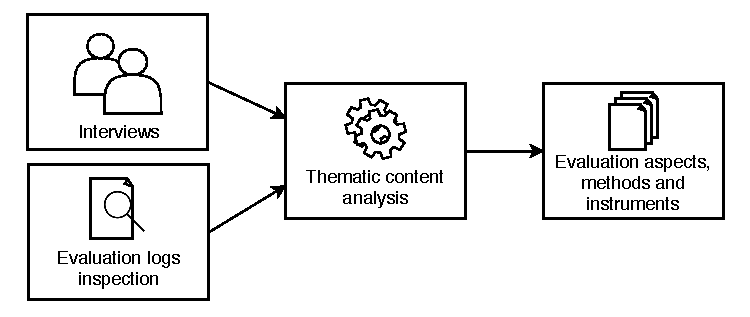
\includegraphics[width=\linewidth]{gfx/aspects/aspectsIdentification}} \quad
\caption{Aspects, methods and instruments identification process}\label{fig:aspectsIdentification}
\end{figure}

\subsection{Analysis}
Collected data is analysed using the thematic analysis method \autocite{Burnard2008}. We produce a list of statements related to the aim of the study. Then, we assign a code to each statement. After that, codes are iteratively grouped to identify potential themes, which are reviewed until defining the four final. 

The initial codes and final themes are presented to the student and three other physiotherapists to validate that the results represented their view. They clarified or added information regarding two statements, though the codes and themes remained the same. The thematic analysis is available online\footnote{Aspects, methods and instruments thematic analysis: \url{https://goo.gl/iJEukN}}.

%-----------------------------------

\section{Aspects, methods and instruments for evaluating PREG}\label{sec:findings_aspects} % Findings -----------------------------------
We identified 46 statements regarding aspects, instruments and methods to evaluate \acp{PREG}. After grouping and categorising the statements iteratively, we identified four final categories: evaluation aspect (31 statements), evaluation instrument (18 statements), evaluation method (8 statements) and evaluation occurrence (1 statement). Some statements belong to more one theme. A summary of teh findings is presented in \autoref{fig:aspectsInstrumentsMethodsIdentificationGraph}.

\begin{figure}[htb]
\myfloatalign
{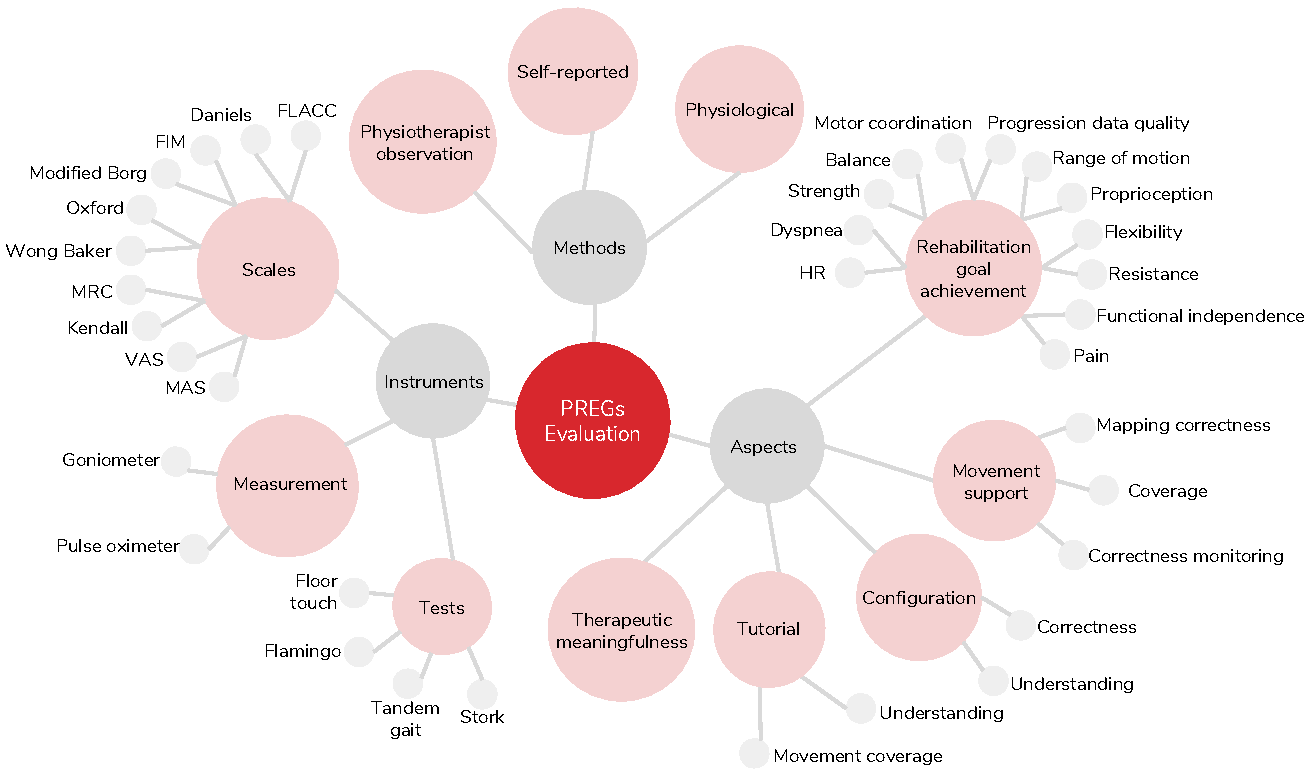
\includegraphics[width=\linewidth]{gfx/aspects/aspectsInstrumentsMethodsIdentificationGraph}} \quad
\caption{Map of qualitative findings, including themes and sub-themes associated to the aspects, methods and instruments identification}\label{fig:aspectsInstrumentsMethodsIdentificationGraph}
\end{figure}

\subsection{Evaluation aspects}
\label{sec:rehab_aspects}
The participants mentioned that the quality of a \ac{PREG} should be measured regarding the impact on patients' progress. They remarked that the highest expectation of patients is to finish their treatments as soon as possible to return to their daily life activities. They highlighted that when a physiotherapist includes something new into the therapy, a patient expects it to be meaningful to their rehabilitation progress. Accordingly, they mentioned different aspects that would allow assessing patients' progress using a \ac{PREG}. These aspects include the range of motion, functional independence, resistance, strength, \ac{HR}, dyspnea, balance, motor coordination, proprioception, flexibility and pain. The selection of aspects to evaluate may depend on the sought after therapeutic goal.

The student validated the correctness of the configuration parameters of each mini \ac{PREG}; i.e., that the configuration parameters produce the expected behaviour. She tested all possible game modes (e.g. movements modes) and verified that each movement was mapped or represented correctly in the mini \ac{PREG}. She suggested including new movements for some mini \acp{PREG}.

Moreover, she assessed that the phrasing of all configuration parameters was understandable for patients and physiotherapists. Furthermore, she tested the relevance of the audiovisual feedback provided by each \ac{PREG} regarding movement correctness.

The student reviewed all mini \acp{PREG}' tutorial; she verified that the phrasing of all instructions was understandable, that all the associated movements were explained and related to a game mechanic. She suggested explaining all movements using graphics and animations.

\subsection{Evaluation methods}
\label{sec:rehab_methods}
The interviews allowed us to identify the following three types of methods for evaluating rehabilitation aspects:

\begin{enumerate}
  \item \emph{Physiotherapist observation}: the evaluation of an aspect depends on the physiotherapist's observation and the criteria of the instrument being employed. For instance, when physiotherapists assess the balance of a patient using the flamingo test \autocite{flamingo}. 
  \item \emph{Self-reported}: patients rate an aspect subjectively, and physiotherapists establish conclusions according to the employed instrument. For instance, patients can rate the pain intensity they are feeling using a \ac{VAS} \autocite{vasScale}.
 \item \emph{Physiological}: physiotherapists collect data directly from patients body; e.g. when they measure the range of motion of a joint.
\end{enumerate}

\subsection{Evaluation instruments}
\label{sec:rehab_instruments}
The participants mentioned some physiotherapy instruments that can be used to evaluate some of the rehabilitation aspects mentioned above. Interviewed physiotherapists expressed that they use the Daniels \autocite{danielsScale}, the \ac{MAS} \autocite{ashwortScale}, the Kendall \autocite{kendallScale}, the Oxford \autocite{oxfordScale} and the \ac{MRC} \autocite{mrcScale} scales to assess muscle strength. They measure pain using the \ac{VAS} \autocite{vasScale}, the \ac{FLACC} \autocite{flaccScale} and the Wong-Baker FACES \autocite{Baker} scales. Also, they use the pulse oximeter to measure \ac{HR} and oxygen saturation. They use the Modified Borg Scale \autocite{modifiedBorgScale_2014} to assess perceived exertion and dyspnea (i.e., shortness of breath). Finally, they expressed that they used the \ac{FIM} \autocite{fim} to assess patients' functional independence and the goniometer \autocite{goniometry} to measure the range of motion. 

Furthermore, they mentioned three tests to assess balance; i.e., the flamingo test \autocite{flamingo}, the tandem gait test \autocite{tandemGaitTest} and the stork test \autocite{storkTest}. The student said that the floor touch test \autocite{floorTouch} can be used to assess flexibility. 

The selection of instruments depends on the therapeutic goal of the evaluated \ac{PREG}. Also, some instruments are of private use, which means that each health institution may have different instruments.

\subsection{Evaluation occurrence}
The physiotherapist expressed that evaluations occur before, during and after treatments take place. That allows diagnosing patients health status and tracking their progress. 

\section{Current practices}\label{sec:current_aspects}

We reviewed 20 published evaluations of \acp{PREG} (or related digital games) to identify evaluation aspects, instruments and methods by frequently employed by evaluators. 16 evaluations assessed \acp{PREG}, \autocite{Celinder2012,Deutsch2011,Rand2008,Brokaw2015,Burke2009,Chang2011,Fitzgerald2008,Hernandez2013,McNeill2012,Ni2014,PirovanoAdvisor2012,Saposnik2010,Seo2016,Shin2014,Sugarman2009,Wuest2014} and 4 assessed digital games for exercise promotion \autocite{Berkovsky2010,Sinclair2010,Zhang2011,Moran2015}.

The most evaluated aspects were enjoyment \autocite{Sinclair2007,Ni2014,Hernandez2013,Berkovsky2010,Shin2014,Moran2015,Chang2011,Rand2008,McNeill2012}, usability \autocite{PirovanoAdvisor2012,Ni2014,Brokaw2015,Rand2008,Fitzgerald2008,McNeill2012}, ease of use \autocite{Wuest2014,PirovanoAdvisor2012,Hernandez2013,Moran2015,Burke2009,Seo2016}, motivation \autocite{Ni2014,Brokaw2015,Shin2014,Chang2011,Seo2016,McNeill2012}, feasibility \autocite{PirovanoAdvisor2012,Sugarman2009,Shin2014,Rand2008,Saposnik2010} and acceptance \autocite{Wuest2014,PirovanoAdvisor2012}. Additional to feasibility and acceptance, we identified 22 new evaluation aspects including perceived exertion \autocite{Berkovsky2010,Chang2011,Rand2008,McNeill2012}, intention to use \autocite{Wuest2014,Moran2015}, adherence \autocite{Wuest2014,PirovanoAdvisor2012}, anxiety \autocite{Moran2015}, clinical score tracking \autocite{Seo2016} and invasiveness \autocite{McNeill2012}.

Regarding evaluation methods, evaluators prefer using ad-hoc questionnaires \autocite{Sinclair2007,Zhang2011,Wuest2014,PirovanoAdvisor2012,Ni2014,Brokaw2015,Hernandez2013,Berkovsky2010,Shin2014,Rand2008,Burke2009,Seo2016}. Also, the \ac{FMA} \autocite{FMAscale} was employed in \autocite{Brokaw2015,Shin2014,Seo2016}, the \ac{ARAT} was employed in \autocite{Shin2014,McNeill2012} and the Modified Borg scale in \autocite{Rand2008,McNeill2012}. Moreover, we identified 19 new instruments including the Berg Balance Scale \autocite{bergScale}, the \ac{MBI} \autocite{mbiScale}, the Motricity Index \autocite{motricityIndex}, the Presence questionnaire \autocite{Witmer2005} and the \ac{TAM} \autocite{Davis1989}.

Finally, the most employed methods include interview \autocite{PirovanoAdvisor2012,Ni2014,Brokaw2015,Celinder2012,Hernandez2013,Shin2014,McNeill2012}, physiotherapy/clinical tests \autocite{Wuest2014,PirovanoAdvisor2012,Brokaw2015,Sugarman2009,Shin2014,Saposnik2010}, physiotherapy/clinical scales \autocite{Brokaw2015,Berkovsky2010,Rand2008,Fitzgerald2008,Saposnik2010} and field observation \autocite{Brokaw2015,Celinder2012,Shin2014,Chang2011}.

The details of each evaluation and the complete list of identified aspects, instruments and methods are available online\footnote{Frequently evaluated aspects, instruments and methods \url{https://goo.gl/EbVGEb}}.

% -----------------------------------------------

\section{Discussion}\label{sec:discussion_aspects} % Discussion %-----------------------------------------------
The aim of this study is to identify aspects that physiotherapists consider important to evaluate \acp{PREG}. Based on the findings, we confirmed that there are rehabilitation aspects that evaluators should consider to assess the impact of \acp{PREG} on patients' treatments. We identified a set of aspects related to rehabilitation goal achievement, movement support, configuration capability, tutorial quality (i.e., user guidance) and therapeutic meaningfulness. Those aspects are relevant to assess if a \ac{PREG} meets physiotherapists and patients needs, and can be used effectively as an assisting methodology in physical therapy. Additionally, we identified a set of methods and instruments to assess those aspects. Additionally, we complemented our findings with the results of reviewing 20 published evaluations of \acp{PREG} and digital games for exertion promotion.

% Progression
The participants remarked that \acp{PREG} should add value to the patients' rehabilitation progress. Therefore, \acp{PREG} should enable patients and physiotherapists to track progression regarding the expected rehabilitation goal. That may imply tracking performance measurements per session; e.g., maximum achieved movement angles or the success rate of correct executed movements. Also, the quality of the tracked data should be assessed. Those results confirm that clinical score tracking is a relevant feature of a rehabilitation game as claimed in \autocite{Seo2016,PirovanoAdvisor2012}.

% Configuration
Additionally, our findings suggest that the configuration capability of \acp{PREG} is important for physiotherapists. According to the student logs, configuration parameters should cover all movements associated with the \ac{PREG}, and the correctness may be assessed by a physiotherapy expert. The configuration capability is relevant since it allows personalising a gameplay session according to a patients' needs, which is important to ensure patients' safety as concluded in \autoref{ch:characterising} and in \autocite{Cameirao2010,Ni2014,Nijholt2008,Wiemeyer2015,Seo2016}.

Additionally, the configuration parameters of a \ac{PREG} should be understandable and easy to use for physiotherapists. In that context, evaluators should assess aspects such as satisfaction \autocite{Sanchez2009,Yanez-Gomez2017,Zhao2016}, ease of use \autocite{Cameirao2010,Moosajee,VandenAbeele2016}, learnability \autocite{Desurvire2009,GonzalezSanchez2009} and acceptance \autocite{Yanez-Gomez2017} involving physiotherapists.

% Associated movements
The physiotherapists and the student's logs suggested that some aspects regarding the \textit{associated movements} of a \ac{PREG} are important. First, movement mapping correctness should be assured since \acp{PREG} use patients' body movements to enable interaction. Second, all movements should be covered by the game mechanics, and patients should consider those movements as meaningful; i.e., the movements should be aligned with the game and therapeutic goals. In that context, evaluators might consider aspects such as accomplishment \autocite{Cameirao2010,Zhao2016} and clarity of goals \autocite{Desurvire2009,VandenAbeele2016}. Third, movement correctness monitoring should be enabled or facilitated by the \ac{PREG}. If the \ac{PREG} is unsupervised, feedback about movement correctness should be automatic, immediate, realistic and specific \autocite{Pasch2009,PirovanoAdvisor2012,Wiemeyer2015}. Otherwise, physiotherapists may need to be able to interrupt gameplay to correct patients. Also, input devices such as motion sensors should enable a meaningful mapping of rehabilitation movements \autocite{Isbister2015}. Finally, the point of view of a \ac{PREG} should allow patients to identify the outcomes of their actions easily.

%Tutorial, ease of use
The tutorial inspection of the student suggests that \acp{PREG} should help patients understand the game goals and rehabilitation movements effectively. That is, patients' attention should be focused on achieving game goals and not on learning how to control the \ac{PREG} \autocite{Isbister2015,Sinclair2007}. Thus, evaluators should assess aspects such as ease of use, learnability \autocite{Desurvire2009,GonzalezSanchez2009}, cognitive load, attention \autocite{Fernandez2008}, clarity of goals \autocite{Desurvire2009,VandenAbeele2016} and absorption \autocite{Lapas2015}. Additionally, the tutorial should cover all associated movements and explains their relation to game mechanics. The quality of tutorials levels should be assessed since patients may have different literacy levels as described in \autoref{sec:reh_patients_constraints}.

%finish as soon as possible, motivation to return to daily life
As expected, the results indicated that \acp{PREG} should be meaningful to patients physical progress. Thus, evaluators should evaluate the capability of \acp{PREG} to contribute to the achievement of the rehabilitation goal. It can be assessed by using the identified rehabilitation aspects, instruments and methods, which are selected depending on the rehabilitation goal. However, evaluators should consider monitoring a group of patients throughout their whole rehabilitation treatments to asses the impact of a \ac{PREG} on patients recovery process properly.

\subsection{Limitations}
The conducted study has some limitations. First, the findings cannot be generalised since the study was qualitative and the source of information was two people. Also, the collected data is based on the experience of the interviewees, one as a physiotherapist and the other as a \ac{PREG} developer (tester). Consequently, there should be more aspects, methods and instruments that may affect the evaluation of \acp{PREG}. Nonetheless, we tried to overcome this limitation by complementing our findings with the information of 20 published evaluations. Finally, most of the results apply to supervised \acp{PREG} since both interviewees based their answers on the idea of including \acp{PREG} in physical therapy at a hospital.

% -----------------------------------------------

\section{Conclusion}\label{sec:conclusion_aspects} % Conclusion -----------------------------------------------
This chapter presented a qualitative study to identify relevant aspects to evaluate \acp{PREG} from the physiotherapy perspective. We confirmed that \ac{GUR} aspects are not sufficient to evaluate \acp{PREG} properly. Evaluators should evaluate if a \ac{PREG} meets physiotherapists and patients expectations and needs. As a result, additional aspects related to the rehabilitation goal assisted by a \ac{PREG} should be assessed; e.g. rehabilitation goal achievement, movement mapping correctness, configuration capability, safety and progress feedback. Also, the ease of use and understanding of the configuration parameters is important to meet physiotherapists expectations. Finally, the ease of use of \acp{PREG} is relevant to avoid patients' distraction from rehabilitation goal. We also identified instruments and methods that may allow evaluating rehabilitation aspects. The findings presented limitations since the conducted study is qualitative and the number of participants is low.
\chapter{A PX Model for \acp{PREG}}
\label{ch:model}
% A model that integrates constraints, aspects, instruments and methods, evaluators and game user researchers will benefit having a model that allows understanding dimensions (ayers and time) and elements that model PX in \acp{PREG}
As presented in \autoref{sec:ox_ux_models}, there are models to study \ac{PX} and \ac{UX}. However, those models are not sufficient to study \acp{PREG} since these do not consider the constraints presented in \autoref{ch:characterising} and the aspects, methods and instruments presented in \autoref{ch:aspects}.

In this chapter, we present a model for studying \ac{PX} in \acp{PREG}, which integrates existing research with the findings presented in this document will allow studying \acp{PREG} properly. The model allows studying existing \ac{PX} aspects and the new aspects that we have identified. Also, it will integrate \acp{PREG} constraints into its components. First, \autoref{sec:related_work_model} presents the \ac{PX} models that we studied to build our model. Then, \autoref{sec:mats_mets_model} describes the methods that we employed to design the model. After that, \autoref{sec:findings_model} describes the proposed model. Finally, \autoref{sec:discussion_model} discusses the findings of the conducted study and \autoref{sec:conclusion_model} concludes the chapter.

% -----------------------------------------------
\section{Related work} % Related work %-----------------------------------------------
\label{sec:related_work_model}
The purpose of this study is to design a model to study \ac{PX} in \acp{PREG}. We have identified some constraints \autoref{ch:characterising} and aspects \autoref{ch:aspects} of \acp{PREG} from the field of physiotherapy. To design a comprehensive model we need to integrate those findings into current \ac{PX} models. Thus, this section presents the models that we considered to design our model.

We presented two models that we considered for our proposal in \autoref{sec:px_ux_models}. First, the \ac{IMP} model \autocite{Elson2014}, which describes \ac{PX} considering three elements, player, context and game. Also, the model suggests that \ac{PX} should be studied before, during and after interaction with a game occurs. Second, the Contextual Gameplay Experience Model \autocite{Engl2013}, which considers three elements similar to those of the \ac{IMP} model and is based on \autocite{Nackea2,Nacked}; i.e., game system, player and contextual influences. In this model, those elements are layers of abstraction, in which contextual influences is the most abstract layer and the game system is the most concrete one. It also suggests that \ac{PX} occurs before, during and after interaction occurs. Below, we present the other models that we use as a base to design our model.

\subsection{A PX Framework}
\textcite{Nackea2} present a \ac{PX} framework based on three layers of abstraction: the context, the player and the game system (See \autoref{fig:px_framework}). Context is the most abstract layer. It comprises the experience resulting from interacting with other players, games and technologies over a certain time. It involves the game community and its generated knowledge. The player layer represents the experience that influences and is influenced by the actions of players. The most concrete layer is the game system and comprises perceivable and technical experience generated by games.

The model presents interrelations among the layers. The context layer shapes players' perceptions of games, e.g., through a bad review. Meanwhile, the player the layer influences the context by generating knowledge about the game. Also, players provide content and data to shape game behaviour and adjust it to their preferences. Finally, the game system layer influences players' experience through its functionality and mechanics.

Finally, the model describes how each layer is affected by time. First, the game system layer is affected by technological changes. Second, the player layer evolves due to psychological and physiological changes. Finally, the context layer changes due to social, political or economic influences.

\begin{figure}[bth]
\myfloatalign
{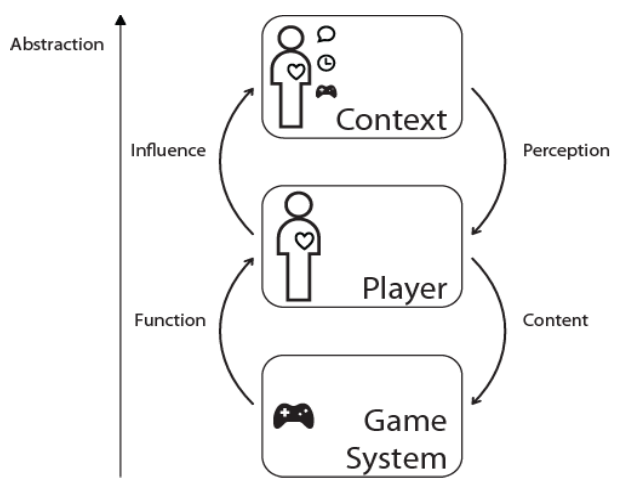
\includegraphics[width=.6\linewidth]{gfx/model/px_framework}} \quad
\caption[The PX Framework]{The \ac{PX} Framework \autocite{Nackea2}}\label{fig:px_framework}
\end{figure}

\subsection{The Game Usability Model}
\textcite{Nacked} presents the Game Usability Model that integrates \ac{PX} research into a single framework. It comprises nine entities that go from theoretical to practical and from concrete to abstract (See \autoref{fig:game_usa_model}). Three of those entities are theoretical constructs that affect \ac{PX}; i.e., technology, player and community. The technology entity is measured by the system quality and analysed using quality assurance. The player entity is measured by gameplay quality and studied using user experience analysis. Finally, the community construct is measured by the social quality and analysed using sociological studies.

This model intends to address three challenges that result when analysing \ac{PX}. The first challenge relates to \ac{PX} optimisation. According to the author, the interface of a game has to optimise \ac{PX} usability and functionality. The second challenge is the complexity of digital games, which are complex software programs due to content, controls, customisation and game design among others. The last challenge relates to time. \ac{PX} should be studied before, during and after interaction occurs. Before interaction, the state of the players and game marketing shape \ac{PX}. Also, the impact of an interaction on a player will affect preceding interactions.

\begin{figure}[bth]
\myfloatalign
{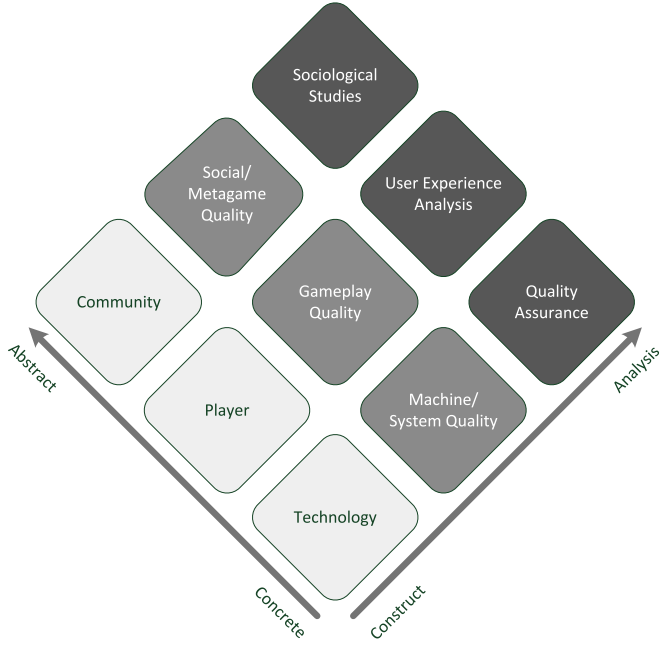
\includegraphics[width=.6\linewidth]{gfx/model/game_usa_model}} \quad
\caption[The Game Usability Model]{The Game Usability Model \autocite{Nacked}}\label{fig:game_usa_model}
\end{figure}

\subsection{The Game Experience Model}
\textcite{Fernandez2008} presents the Game Experience Model which suggests that the main result of game experience is fun. The model is based on three stages. First, the antecedents stage intends to capture the elements that motivate players to play a game, and lead to certain behaviours during an interaction. Second, the processing stage refers to the interaction moment between a player and a game. This stage depends on the players' motivation to play. Third, fun depends on the consequences of interacting with a game. These consequences can be cognitive such as thoughts and inferences, or emotional such as feelings.

The antecedents comprise players' demographics and game activity; i.e., previous experiences, game and hardware preferences and purpose. Those elements affect the motivation of players to start or continue playing a game.

Players' motivation determines the degree of attention and effort that they invest in a game during processing. According to the author, motivation also determines if players play using a serious or playful strategy. Additionally, games have pragmatic and hedonic attributes that affect \ac{PX}. Pragmatic attributes are assessed through the game interface and usability while hedonic attributes comprise the game mechanics (universe), the game features that trigger interactivity and the technology.

In \autocite{Fernandez}, the author conducted a study to prove the relations among the different elements of its model. The results showed that the years playing games and game genre preference define the user profile and purpose. Also, the author found that the user profile is related to motivation, but does not explain it. Furthermore, the results showed that when players are motivated, they can overcome usability shortcomings. Finally, the author found that high-quality technology and usability lead to universe appreciation.

\subsection{The Contextual Game Experience Model}
\textcite{Mayra} describes a model that considers the socio-cultural context of \ac{PX}. The author argues that games are played not only to experience fun, but also to facilitate social situations; e.g., when used to maintain or strengthen social relations. According to this model, the game experience is pre-defined, modified and post-defined by multiple dimensions. It relates to the immediate personal and social contexts. Thus, knowing players motivations, game habits and historical reasons to play is important to understand \ac{PX}. Additionally, the contexts for digital game production, the contexts provided by earlier forms for play (i.e., people's game literacy) and the context of social norms and values influence each other and shape game experience.

\subsection{People, Places and Play Research Framework}
\textcite{DeKort2007b} present a research framework that explores game experience as a situated experience formed by co-players, audience and spatial organisation. That is, the game experience is influenced by social contexts. The model is based on the evidence that people have better experiences when playing with or against players since social settings empower or diminish emotions. The social context of gaming comprises the presence of others, their ability to monitor and communicate with players, their role in the system (i.e., co-players or audience) and their relationships.

%-----------------------------------
%\section{Aim of the study} % Aim of the study -----------------------------------

%-----------------------------------

\subsection{The Elements of \ac{PX}}

\textcite{Ferrara} presents a model to design and understand digital games. The model is divided into five planes, which have an associated short-term and long-term element. The planes should be addressed in the order presented below:

\begin{enumerate}
    \item \emph{Motivation}: it represents the players and their reasons to play a game. The short-term element is the \textit{players' interest} in the game, and the long-term elements are \textit{game rewards} that sustain interest over time.
    \item \emph{Meaningful choices}: it represents the mechanics that enable players to decide on the outcomes of game events. The short-term element is the players' \textit{strategy} and the long-term elements are the players' \textit{tactics}.
    \item \emph{Balance}: it refers to the appropriate level of challenge that players perceive as fair and equitable. The short and long-term elements are the game variables that enable balance.
    \item \emph{Usability}: it refers to the \ac{UX} and usability aspects of games. The short-term element of this plane is the players' sense of \textit{control}, and the long-term is the players' sense of \textit{mastery}.
    \item \emph{Aesthetics}: it refers to the aesthetic design of games. The short-term element is the players' \textit{sensory} perception of games (e.g., visual, haptic, audio), and the long-term element is the players' \textit{contemplative} perception of narrative.
\end{enumerate}

\section{Model definition study} % Materials -----------------------------------
\label{sec:mats_mets_model}
\subsection{Aim of the study}
A study to propose a comprehensive model of \ac{PX} to evaluate \acp{PREG} is conducted. That is, to define a model that integrates current research in \ac{PX} and the characteristics and constraints of \acp{PREG} that we identified in \autoref{ch:characterising}.

\subsection{Procedure}
First, a literature review to identify existing \ac{PX} models is conducted. The models that serve to study \ac{PX}, game experience or gameplay experience are included. The eight documents presented in \autoref{sec:related_work_model}are selected. Four documents are identified in Scopus, and the remaining are extracted from their references. Then, the documents are reviewed and analysed to identify common \ac{PX} constructs a design a preliminary model. After that, the findings of the study that we presented in \autoref{ch:characterising} are mapped into the preliminary model to design the final one. An overview of the procedure is presented in \autoref{fig:modelDefiniton}.

\begin{figure}[bth]
\myfloatalign
{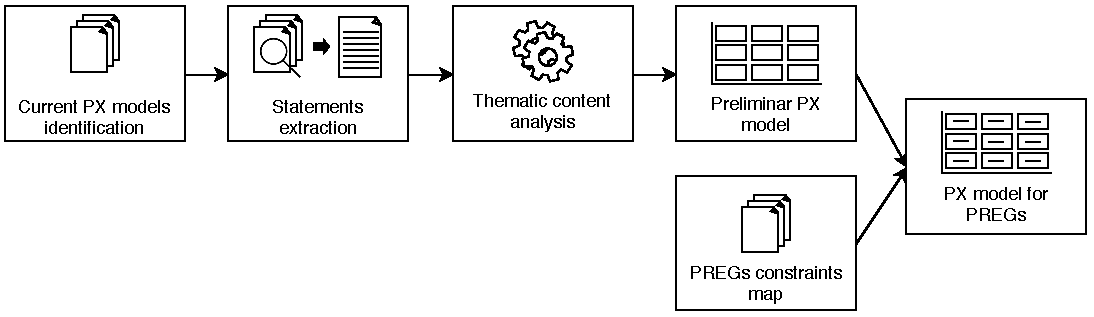
\includegraphics[width=\linewidth]{gfx/model/modelDefiniton}} \quad
\caption{Overview of model definition procedure}\label{fig:modelDefiniton}
\end{figure}

\subsubsection{Analysis}
The documents are analysed using the thematic analysis method \autocite{Braun}. The analysis is 'theory-driven' since we have identified a target data; i.e., \ac{PX} constructs and dimensions. The documents are reviewed to produce a list of relevant statements; i.e., those that are closely related to the aim of the study. Each statement was registered in a list including a reference to its source document. Then, preliminary codes are assigned to the statements. After that, the codes are iteratively grouped to identify potential themes, which are reviewed until defining the three final.

The thematic analysis of the reviewed documents \footnote{Existing PX models thematic analysis: \url{https://goo.gl/QvtG9G}} and the mapping of the \acp{PREG} constraints \footnote{PREGs constraints mapping into the PX model: \url{https://goo.gl/wdn57M}} are available online.

%-----------------------------------
\subsection{PX Model for PREGs} % Findings -----------------------------------
\label{sec:findings_model}
After conducting the thematic analysis, 104 initial codes were identified and iteratively grouped until we achieved a total of three main themes. The first theme is \textit{layers of abstraction} which represent the main actors that may influence \ac{PX}. The second theme is \textit{moments of \ac{PX}}, which represents the moments in which \ac{PX} should be studied. The last theme refers to the relations among the first two themes.

\subsubsection{Layers of abstraction}
\label{sec:layers_abstraction}
The layers of abstraction represent the actors that influence \ac{PX} \autocite{Nacked,Nackea2,Engl2013,Elson2014}. In this study, we identified three main layers of abstraction; i.e., \textit{the context, the player} and \textit{the game system}. \ac{PX} should be studied in a situational perspective \autocite{Nacked,DeKort2007b} since it influences players' perceptions \autocite{Elson2014} behaviours and interactions \autocite{Engl2013,DeKort2007b}. \ac{PX} represents the individual experience of playing a game \autocite{Engl2013,Nackea2}, that is, every experience is shaped by the unique perspective \autocite{Fernandez2008} and properties \autocite{Nacked} of each player. Lastly, games are designed to offer pleasurable experiences to players, although these are complex pieces of software \autocite{Nackea}, and may have numerous interaction possibilities, challenges and complex controls \autocite{Nacked} that alter \ac{PX}.

Although \textcite{Nackea2} proposed a set of relations among the three layers of abstraction,which we described previously; we identified new relations regarding the use of \acp{PREG} in physical therapy. In that case, the game system assists physical therapy, and physiotherapists shape \ac{PX} by configuring the game system and supervising players. The layers of abstraction and their relations are illustrated in \autoref{fig:layersOfAbstraction}.

\begin{figure}[bth]
\myfloatalign
{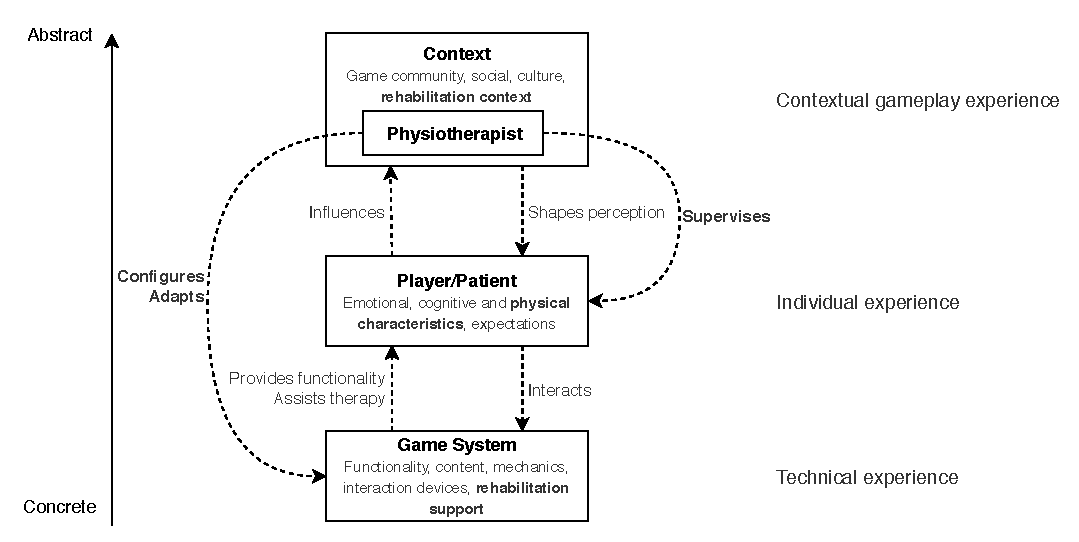
\includegraphics[width=\linewidth]{gfx/model/layersOfAbstraction}} \quad
\caption{\ac{PX} layers of abstraction and relations among them} \label{fig:layersOfAbstraction}
\end{figure}

\subsubsection*{Context}

The \textit{Context} is the most abstract layer and forms the contextual gameplay experience and may empower player's positive emotions and enhance or diminish their negative ones \autocite{DeKort2007b}. It shapes the experience of players through environmental influences that affect players' motivation to play a game \autocite{Elson2014}. Studying the context layer in the long-term may imply conducting sociological studies \autocite{Nacked}.

The social context of playing games \autocite{Mayra,DeKort2007b,Elson2014} comprises the influence of other people. First, co-players presence \autocite{Nacked,Nackea2,Nackea,DeKort2007b,Elson2014,Mayra} (i.e., co-located, mediated, simulated or absent) may enhance \ac{PX} depending on players preferences \autocite{DeKort2007b}. Similarly, the presence of an audience; i.e., people that monitors players' actions and emotions, may influence \ac{PX} \autocite{DeKort2007b,Mayra,Nackea2}. In the case of \acp{PREG}, physiotherapists represent a permanent audience that should be studied when evaluating \ac{PX}. 

Furthermore, game communities \autocite{Nacked,Nackea2,Elson2014} shape the social quality of games; these enable players to interact with others using different forms of communication \autocite{Elson2014}, and offer opportunities for review and discussion \autocite{Nacked}. Consequently, game communities influence players perception of certain games or games genres \autocite{Nackea,Nackea2}. Likewise, the game market \autocite{Elson2014,Nackea} influences players preferences and choice.

When playing a game, the location \autocite{Engl2013,Elson2014}, spatial organisation \autocite{DeKort2007b} and technical infrastructure \autocite{Elson2014} may enhance or diminish the experience. This is relevant for \acp{PREG} sine these employ interaction devices such the Kinect, thereby requiring enough space to locate players at an adequate distance.

Moreover, cultural parameters such as values and norms \autocite{Elson2014,Mayra} may allow or prevent playing a game.

The rehabilitation context constraints presented in \autoref{sec:reh_context_constraints} may extend this layer. These constraints include institutions norms and regulations, physiotherapists' participation, the use of assisting objects and therapy related activities.

The context layer changes based on sociological, economic or political changes that affect players \autocite{Nackea2}.

\subsubsection*{Player/Patient}

The \textit{Player} layer represents the individual experience of a person when playing a game. This layer comprises the characteristics of s player as individual \autocite{Elson2014} such as his/her cultural \autocite{Elson2014} and historical \autocite{Mayra} background, demographic data (e.g, age, gender, literacy) \autocite{Elson2014,Fernandez2008,Ferrara} and personal traits \autocite{Elson2014}. Analysing players' characteristics is important to offer a compelling experience since each kind of player may have different expectations. For instance, playful oriented players are curious, explorers and focused on the present, whereas the serious oriented players are goal oriented and focus efforts on the future \autocite{Fernandez2008}.

Also, this layer involves factors related to previous gaming experiences of a player including memories \autocite{Elson2014}, game activity (e.g. games and hardware preferences/aversions, time playing and frequency) \autocite{Fernandez2008,Nackea2,Nacked,Mayra} and games literacy \autocite{Mayra}.

In addition to entertainment, a player may start playing a game with other purposes such as socialising, training and rehabilitating. Accordingly, the player layer comprises the motivations and expectations of a player that are not related to the game itself; these include the need for interaction, relatedness or affiliation \autocite{DeKort2007b,Mayra}, and the need to rehabilitate using \acp{PREG}.

Furthermore, this layer includes the processes and responses that players experience during and after playing a game. The processes and responses can be emotional such as fun, motivation, pleasure, engagement, \autocite{Fernandez2008,Ferrara} and enjoyment \autocite{Nacked}; cognitive such as mastery, control \autocite{Ferrara}, attention, thoughts and opinions \autocite{Fernandez2008}; and physical such as \c{HR}, motion range and balance.

In the case of \acp{PREG}, the physical processes and responses are relevant since players are recovering from a physical impairment. Moreover, the player layer comprises the patients' related constraints presented in \autoref{sec:reh_patients_constraints}.

The player/patient layer changes gradually over time based on psychological and physiological processes experienced by players \autocite{Nackea2}.

\subsubsection*{Game System}
The \textit{Game System} is the most concrete layer and represents the perceivable and technical experience elicited when playing a game \autocite{Nackea2,Elson2014,Nackea,Nacked}. This layer depends on technological limits or advances to evolve \autocite{Fernandez2008}. Studying the game system in \ac{PX} is important since a game is a complex software system \autocite{Mayra,Nackea} and its design impacts directly on the experience that a player may have.

This layer comprises general prerequisites to ensure the availability of a game; this includes attraction factors \autocite{Elson2014}, \ac{QA} \autocite{Nacked} and the learning curve, which should meet players skills to avoid frustration \autocite{Nacked}. The general prerequisites may involve technical \autocite{Fernandez2008,Engl2013,Nackea2} and marketing \autocite{Nacked} issues.

Furthermore, the game system layer includes interactive characteristics such as game design \autocite{Nacked}, content \autocite{Elson2014,Nackea2,Fernandez2008}, mechanics \autocite{Elson2014,Ferrara}, rules \autocite{Nackea}, universe (i.e., plot, characters and realism) \autocite{Fernandez2008,Ferrara}, interface, media \autocite{DeKort2007b,Fernandez2008}, aesthetics \autocite{Ferrara}, playability \autocite{Engl2013,Fernandez2008} and interactivity (i.e., game challenge, pace and responsiveness) \autocite{Fernandez2008}. Additionally, this layer involves the game technology \autocite{Engl2013,Fernandez2008}; i.e., the interaction devices.

The game system comprises the components that assist a rehabilitation therapy. It involves the interaction devices constraints presented in \autoref{sec:interation_dev_constraints}. And the constraints presented in \autoref{sec:reh_goal_constraints} that impose prerequisites on the game system such as patients' safety assurance, feedback provision about progress and exercise correctness, movement mapping correctness and gameplay time.

The game system layer changes over time according to technological steps, which are mainly imposed by consoles manufacturers \autocite{Nackea,Nackea2}.

\subsubsection{Moments of \ac{PX}}
We identified that \ac{PX} is a comprehensive phenomenon that occurs not only during the actual gameplay \autocite{Mayra}; thus, it should be studied along three moments \autocite{Elson2014,Fernandez2008,Nackea2,Nackea,Nacked} (i.e., before, during and after playing a game). \textcite{Elson2014} name these three moments pre-game, game and post-game effects; whereas \textcite{Fernandez2008} names them antecedents, processing and consequences. Moreover, \textcite{Mayra} claims that \ac{PX} is pre-defined, modified and post-defined by multiple dimensions. We name these moments as \textit{antecedents, interaction} and \textit{effects} since those represent what each moment refers to. The moments of \ac{PX} and their relation are illustrated in \autoref{fig:temporalDimension}.

\begin{figure}[bth]
\myfloatalign
{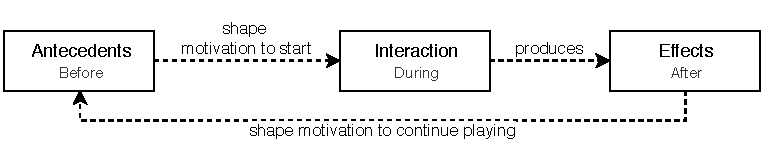
\includegraphics[width=.9\linewidth]{gfx/model/temporalDimension}} \quad
\caption{Moments of \ac{PX}}\label{fig:temporalDimension}
\end{figure}

\subsubsection*{Antecedents}
The antecedents are everything that occurs before the actual gameplay and shape players' motivation to start playing a game \autocite{Fernandez2008,Ferrara}. In the case of \acp{PREG}, the antecedents shape physiotherapists' motivation to use a game in physical therapy.

\subsubsection*{Interaction}
The interaction depends on the antecedents and occurs when players play a digital game \autocite{Elson2014,Fernandez2008,Nacked}. This moment shapes the players' perception of a game depending on their experience \autocite{Fernandez2008}. In \acp{PREG}, the interaction moment would also affect physiotherapists' perception. The effects of interaction have a direct impact on future experiences.

\subsubsection*{Effects}
The effects are positive or negative consequences that result from the interaction moment \autocite{Fernandez2008}; these form a feedback loop that affects future interactions \autocite{Nacked,Elson2014} shaping players' motivation to continue playing a game. The effects can be short-term and long-term. Short-term effects are temporary changes in thoughts, feelings and behaviours right after an interaction. Whereas, long-term effects are consequences of repeated episodes of interaction \autocite{Elson2014}.

\subsubsection{Layers of abstraction over the moments of \ac{PX}}
\label{sec:rel_among_dimensions}
The layers of abstraction can be studied throughout the moments of \ac{PX}. We mapped the layers' components that we present previously (See \autoref{sec:layers_abstraction}) into these moments as illustrated in \autoref{fig:pxModel} and described below.

\begin{figure}[bth]
\myfloatalign
{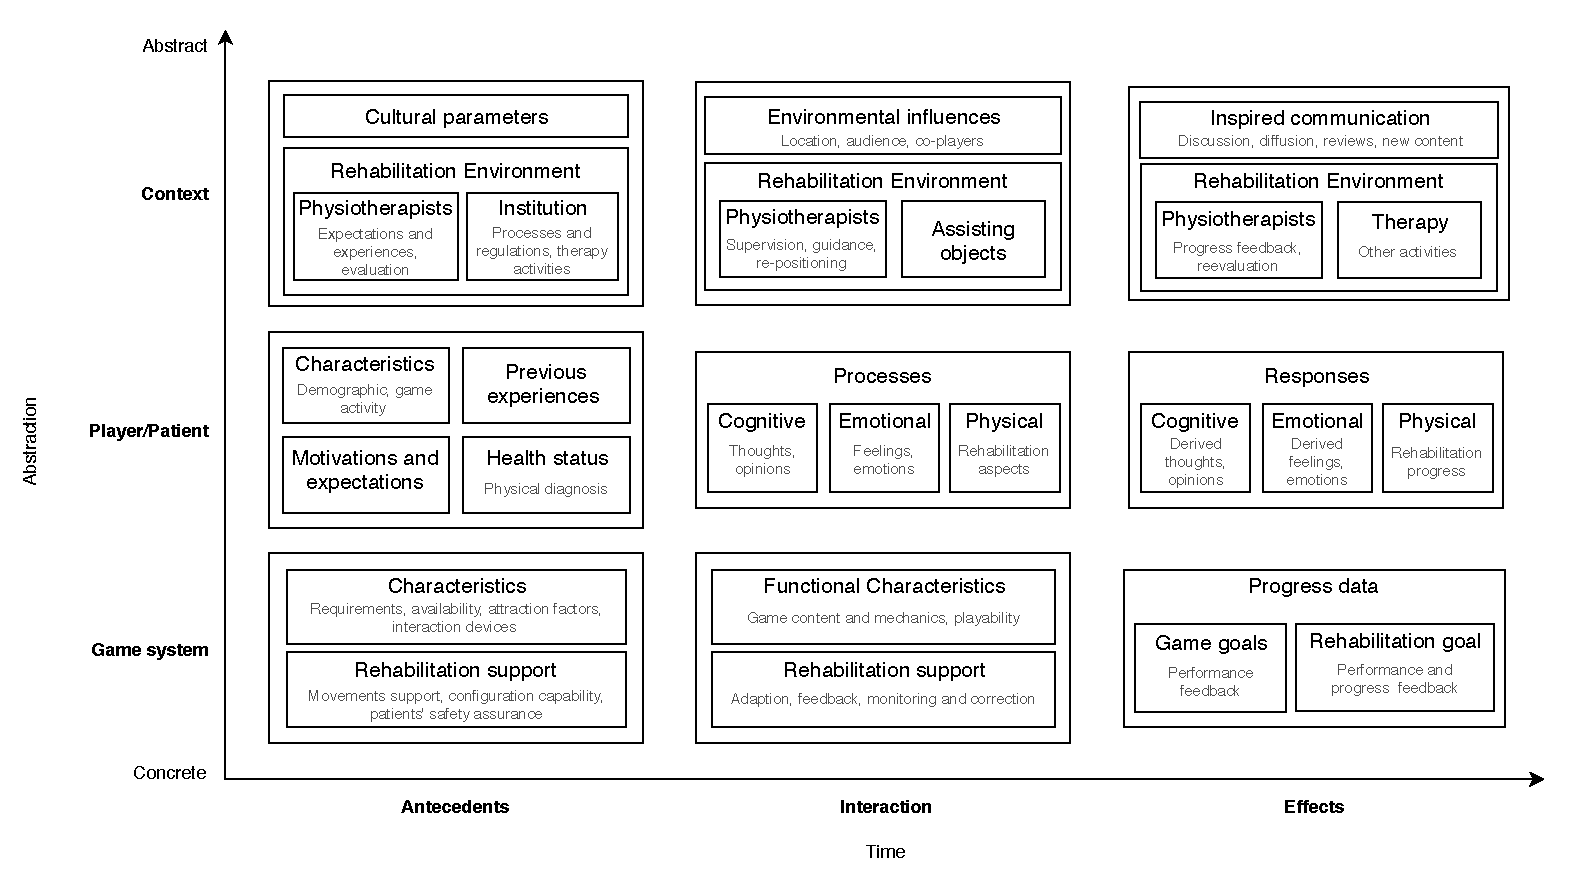
\includegraphics[width=\linewidth]{gfx/model/pxModel}} \quad
\caption{\ac{PX} Layers of Abstraction over Time}\label{fig:pxModel}
\end{figure}

\subsubsection*{Layers of abstraction during the antecedents}
During the antecedents, the \textit{context} comprises the elements affect players' opportunity of playing a game. That includes cultural parameters, the game community, the health institution regulations and physiotherapists' expectations, criteria and experience with \acp{PREG}.

The \textit{player/patient} layer is defined by player's characteristics, game experience, motivations and expectations (including those regarding their physical therapy and the use of \acp{PREG}) and health status (i.e., impairment, physical skills, functional independence). 

On the other hand, the \textit{game system} layer comprises general prerequisites of games such as \ac{QA} and attraction factors. In physical rehabilitation, it comprises the capability of the game to assist treatments.

\subsubsection*{Layers of abstraction during the interaction}
During the interaction, the \textit{context} layer includes influences from the environment and the rehabilitation process (e.g. physiotherapists participation and use of assisting object). The \textit{player/patient} layer comprises the sum of cognitive, emotional and physical processes and behaviours experienced by players while playing a game. Lastly, the \textit{game system} layer comprises the characteristics that enable interaction and rehabilitation (adaptation, feedback provision, monitoring, exercise correction and physical objects support).

\subsubsection*{Layers of abstraction during the effects}
The effects of the \textit{context} layer include all forms of communication caused or inspired by playing a game, including the physiotherapists' feedback and re-evaluation and other therapy related tasks such as paper-work. The \textit{player/patient} layer effects comprise cognitive, emotional and physical responses derived from an interaction episode. The physical responses are associated with the expected rehabilitation goal. The \textit{game system} layer comprises the quality of progress data regarding game and rehabilitation goals.

% -----------------------------------------------
\section{A Methodology to Evaluate PX in PREGs}
\label{sec:methodology}
Evaluating \ac{PX} in \acp{PREG} requires using a methodology that matches the model that we presented in the previous section. An evaluation may cover one or more moments and layers of abstraction of \ac{PX}. Also, the aspects to be assessed depend on the moments and layers being evaluated. Evaluators should select the adequate methods and instruments to evaluate those aspects properly. Lastly, such methodology may enable iterative evaluations since \ac{PX} evolves after each interaction of a player with a game. For instance, to evaluate the impact of a \ac{PREG} on a patient's rehabilitation process, an evaluator should assess the \textit{player/patient} layer throughout the three moments of \ac{PX}, during a whole treatment. The evaluator should identify relevant aspects to evaluate such as range of motion, which can be assessed using goniometry. Those aspects may be measured before, during and after several interaction episodes.

In this section, we present a methodology that attempts to guide evaluators in the process of selecting evaluation aspects, methods and instruments to assess \ac{PX} in \acp{PREG}. This methodology is intended to be used along the whole development life cycle. It can be used iteratively to refine the outcomes of each stage after each evaluation. The stages of our methodology are illustrated in \autoref{fig:PXEvaluationMethodology} and detailed below.

\begin{figure}[bth]
\myfloatalign
{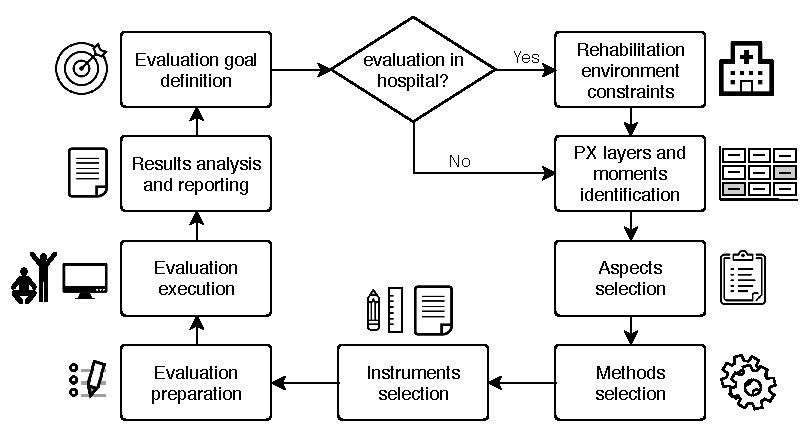
\includegraphics[width=\linewidth]{gfx/model/PXEvaluationMethodology}} \quad
\caption{Stages of the proposed methodology}\label{fig:PXEvaluationMethodology}
\end{figure}

\subsection{Evaluation goal definition}
Evaluators should now define the evaluation goal based on the development maturity of the \ac{PREG}. First, evaluators should focus on assuring patient’s safety. First, they should concentrate on the evaluating the antecedents of \ac{PX}; and then they can start assessing the interaction and effects moments of \ac{PX}.

\subsection{Rehabilitation environment constraints}
If required, evaluators should identify constraints additional to those presented in \autoref{ch:characterising}; these include constraints imposed by regulations and internal processes of the health institution where evaluation may occur. They should concentrate on the logistics that are required to perform an evaluation including participants, location, regulations, among others. When a \ac{PREG} consists of collection of mini-games, each mini-game should be evaluated separately.

\subsection{\ac{PX} layers and moments identification}
Evaluators identify which layers of abstraction and moments of \ac{PX} should be evaluated to achieve the evaluation goal established in the previous stage.

\subsection{Evaluation aspects selection}
Selecting the aspects to be evaluated is a crucial task to be overcome when preparing an evaluation. This selection depends on the layers and moments of \ac{PX} to be evaluated, the available resources and the development maturity of the evaluated \ac{PREG}. A discussion about relevant aspects to be evaluated in \acp{PREG} was presented in \autoref{sec:rehab_aspects}. \autoref{tab:aspectsModelMappingContext}, \autoref{tab:aspectsModelMappingPlayer} and \autoref{tab:aspectsModelMappingGame} present a mapping between those aspects and each moment of \ac{PX} for the context, the player/patient and the game system layers of abstraction respectively. A mapping that includes a larger set of aspects is available online \footnote{Mapping of evaluation aspects into the PX Model: \url{https://goo.gl/K4rked}}

\begin{table}[h]
\caption{Aspects to evaluate the context layer over time}
\label{tab:aspectsModelMappingContext}
\myfloatalign
\resizebox{0.9\linewidth}{!}{
\begin{tabular}{p{7cm}llp{2cm}}
\toprule
\multirow{2}{*}{\spacedlowsmallcaps{Aspect(s)}} & \multicolumn{3}{c}{\spacedlowsmallcaps{Moment of PX}} \\
\cline{2-4}
 & \spacedlowsmallcaps{Antecedents} & \spacedlowsmallcaps{Interaction} & \spacedlowsmallcaps{Effects} \\
\midrule
Physiotherapists preference, expectations & X &  &  \\
\midrule
Game diffusion & X &  & X \\
\midrule
Location & X & X &  \\
\midrule
Competence, collaboration &  & X &  \\
\midrule
Game knowledge generation &  &  & X \\
\midrule
Institutions regulations/processes & X &  &\\
\midrule
\bottomrule
\end{tabular}}
\end{table}

\begin{table}[h]
\caption{Aspects to evaluate the player/patient layer over time}
\label{tab:aspectsModelMappingPlayer}
\myfloatalign
\resizebox{\linewidth}{!}{
\begin{tabular}{p{10cm}llp{2cm}}
\toprule
\multirow{2}{*}{\spacedlowsmallcaps{Aspect(s)}} & \multicolumn{3}{c}{\spacedlowsmallcaps{Moment of PX}} \\
\cline{2-4}
 & \spacedlowsmallcaps{Antecedents} & \spacedlowsmallcaps{Interaction} & \spacedlowsmallcaps{Effects} \\
\midrule
Emotion & X & X & X \\ \midrule
Negative-positive affect &  & X & X \\ \midrule
Interest & X & X & X \\ \midrule
Story & X & X &  \\ \midrule
Accomplishment &  & X & X \\ \midrule
Engagement, challenge, flow, enjoyment, fun, immersion, absorption, presence, attention, tension, curiosity &  & X &  \\ \midrule
Clarity of game goals, ease of use, cognitive load, learnability &  & X &  \\ \midrule
Preference & X &  & X \\ \midrule
Rehabilitation goal achievement &  &  & X \\ \midrule
Physical rehabilitation aspects & X & X* & X \\ \midrule
Movement meaningfulness &  & X &  \\ \midrule
Tutorial understanding &  & X &  \\
\midrule
\bottomrule
\end{tabular}}
\\ * If supported by the \ac{PREG} or other equipment
\end{table}

\begin{table}[htb]
\caption{Aspects to evaluate the game system layer over time}
\label{tab:aspectsModelMappingGame}
\myfloatalign
\resizebox{0.9\linewidth}{!}{
\begin{tabular}{p{7cm}llp{2cm}}
\toprule
\multirow{2}{*}{\spacedlowsmallcaps{Aspect(s)}} & \multicolumn{3}{c}{\spacedlowsmallcaps{Moment of PX}} \\
\cline{2-4}
 & \spacedlowsmallcaps{Antecedents} & \spacedlowsmallcaps{Interaction} & \spacedlowsmallcaps{Effects} \\
\midrule
Playability & X & X & X \\ \midrule
Configuration capability & X &  &  \\ \midrule
Adaptation capability &  & X &  \\ \midrule
Movement mapping correctness & X &  &  \\ \midrule
Movement mapping completeness & X &  &  \\ \midrule
Monitoring, movement correction, movement correctness feedback &  & X & \\ \midrule
Progress feedback &  & X & X \\ \midrule
Tutorial completeness & X &  &  \\ \midrule
Functionality, aesthetics, point of view &  & X &  \\ \midrule
\bottomrule
\end{tabular}}
\end{table}

\subsection{Evaluation methods selection}
Evaluators should select methods based on the selected aspects and available re-sources; e.g., experts, participants, location and evaluation instruments. A discussion about relevant methods to evaluate in \acp{PREG} was presented in \autoref{sec:rehab_methods}. Moreover, \autoref{tab:methodsModelMappingContext}, \autoref{tab:methodsModelMappingPlayer} and \autoref{tab:methodsModelMappingGame} present the methods that evaluators can use to assess the context, the player/patient and the game system layers of abstraction respectively, during each moment of \ac{PX}.

\begin{table}[htb]
\caption{Evaluation methods for the context layer over time}
\label{tab:methodsModelMappingContext}
\myfloatalign
\resizebox{0.8\linewidth}{!}{
\begin{tabular}{p{6cm}llp{2cm}}
\toprule
\multirow{2}{*}{\spacedlowsmallcaps{Method}} & \multicolumn{3}{c}{\spacedlowsmallcaps{Moment of PX}} \\
\cline{2-4}
 & \spacedlowsmallcaps{Antecedents} & \spacedlowsmallcaps{Interaction} & \spacedlowsmallcaps{Effects} \\
\midrule
Questionnaires & X & X & X \\ \midrule
Interview & X &  & X \\ \midrule
Field-Behavioural observation & X & X &  \\ \midrule
Focus groups & X &  & X \\ \midrule
Co-discovery learning &  & X &  \\ \midrule
Peer tutoring &  & X &  \\ \midrule
Prisoner dilemma task &  & X &  \\ \midrule
Ethnography & X & X & X \\ \midrule
Cultural debugging & X &  &  \\ \midrule
Multiplayer game metrics &  & X &  \\ \midrule
\bottomrule
\end{tabular}}
\end{table}

\begin{table}[h]
\caption{Evaluation methods for the player/patient layer over time}
\label{tab:methodsModelMappingPlayer}
\myfloatalign
\resizebox{0.8\linewidth}{!}{
\begin{tabular}{p{6cm}llp{2cm}}
\toprule
\multirow{2}{*}{\spacedlowsmallcaps{Method}} & \multicolumn{3}{c}{\spacedlowsmallcaps{Moment of PX}} \\
\cline{2-4}
 & \spacedlowsmallcaps{Antecedents} & \spacedlowsmallcaps{Interaction} & \spacedlowsmallcaps{Effects} \\
\midrule
Questionnaires & X & X & X \\ \midrule
Interview & X &  & X \\ \midrule
Video recording &  & X &  \\ \midrule
Field-Behavioural observation & X & X & X \\ \midrule
Think-aloud protocol &  & X &  \\ \midrule
Focus groups & X & X & X \\ \midrule
Question-asking protocol &  & X &  \\ \midrule
Biometrics analyse & X &  & X \\ \midrule
\ac{EEG}, \ac{EMG}, \ac{EDA}, \ac{HR} & X & X & X \\ \midrule
Body movement coding &  & X &  \\ \midrule
Eye-tracking &  & X &  \\ \midrule
Persona modelling & X &  &  \\ \midrule
Player modelling & X &  &  \\ \midrule
Physical rehabilitation tests & X &  & X \\ \midrule
Physiotherapist observation & X & X & X \\ \midrule
\bottomrule
\end{tabular}}
\end{table}


\begin{table}[htb]
\caption{Evaluation methods for the game system layer over time}
\label{tab:methodsModelMappingGame}
\myfloatalign
\resizebox{0.8\linewidth}{!}{
\begin{tabular}{p{6cm}llp{2cm}}
\toprule
\multirow{2}{*}{\spacedlowsmallcaps{Method}} & \multicolumn{3}{c}{\spacedlowsmallcaps{Moment of PX}} \\
\cline{2-4}
 & \spacedlowsmallcaps{Antecedents} & \spacedlowsmallcaps{Interaction} & \spacedlowsmallcaps{Effects} \\
\midrule
\ac{QA} & X & & \\ \midrule
\ac{RITE} & X & X &  \\ \midrule
Heuristic evaluation & X & X & X \\ \midrule
Guidelines or standard inspections & X & X & X \\ \midrule
Cognitive walkthrough & X & X & X \\ \midrule
Pluralistic walkthrough & X & X & X \\ \midrule
Gameplay metrics &  & X &  \\ \midrule
Game logs &  & X &  \\ \midrule
A/B Testing & X & X & X \\ \midrule
\bottomrule
\end{tabular}}
\end{table}

\subsection{Evaluation instruments selection}
Evaluators should select evaluation instruments based on the aspects and methods involved in the evaluation. Evaluation instruments for \acp{PREG} may be borrowed from \ac{GUR}, \ac{UX} and physical rehabilitation fields. A discussion about relevant instruments to evaluate in \acp{PREG} was presented in \autoref{sec:rehab_instruments}. Additionally, a mapping between evaluation aspects and instruments is available online \footnote{Mapping between evaluation aspects and instruments: \url{https://goo.gl/j9suDc}}

\subsection{Evaluation preparation}
Evaluators should prepare all logistics associated to evaluation and a test protocol based on the outcomes of the previous stages.

\subsection{Evaluation execution}
Evaluators conduct the planned evaluation. The evaluation may occur in a laboratory or at a health institution.

\subsection{Results analysis and reporting}
Evaluators analyse the data collected during evaluation and reports the findings and recommendations considering the evaluation goal. This is a common task on usability and \ac{UX} evaluation; thus, similar approaches can be employed.


\section{Discussion} % Discussion %-----------------------------------------------
\label{sec:discussion_model}
%%%%% Reiterate the Research Problem/State the Major Findings:
% Comprehensive model for \acp{PREG}
% PX studied in two dimensions: time: before, during, after; level of abstraction: context, player/patient, game system + constraints identified in previous study
% Integrate models to explain relations among layers and dimensions of \a{PX}
Although there are models to study \ac{PX} for game systems, those do not integrate constraints derived from the use of \acp{PREG} since the models were constructed based on entertainment games. Therefore, we conducted a qualitative study to explore the constructs and concepts of existing \ac{PX} models and integrate them with the rehabilitation constraints that we identified in a previous study (See \autoref{ch:characterising}). The purpose of the study was to design a comprehensive model to study and understand \ac{PX} in \acp{PREG}. The model is constructed by two dimensions, time and level of abstraction. 

%-----discuss regarding requirements by  \autocite{Nackea}
% must provide broad and inclusive layers that focus on player and game evaluation;
%each of the layers should include at least one emerging methodology for game evaluation
%the model should be applicable to stages of the development process of digital game
%ideally allowing for each layer to be tested iteratively but at the same time.

%%%%%%% Explain the Meaning of the Findings and Why They are Important: expected? unexpected? (explain these especially). unusual or unanticipated patterns or trends that emerged from your results and explain their meaning in relation to the research problem.
% PX study as an iterative process, consequences affect -> future antecedents
Regarding the time dimension, \ac{PX} should be studied considering three moments: its antecedents (before), the interaction itself (during) and its effects (after), which is similar to \ac{UX} \autocite{iso9241:210}. As a consequence, studying or evaluating \ac{PX} may represent an iterative process since the effects of a interaction become the antecedents of future experiences.

About abstraction, three levels were identified in the literature, the context, the player and the game system. The context was enriched with rehabilitation environment constraints represented in institutions, physiotherapists and therapy activities. The player layer was enriched including characteristics of players as patients of rehabilitation therapies. Finally, the game system was extended with requirements that an exergame should meet to offer an experience in rehabilitation therapies.

% Expected: important role of physios adn insitutions as antecedents to trigger interaction, physios as partipators of interaction and progress feedback (/)
% consider physiotherapists vision (clinical(evaluators) and as users)
As expected, our findings remarked the role of the rehabilitation context at each moment of \ac{PX}. Particularly, it allows identifying when physiotherapists play a role of users (e.g. when configuring a game) or as evaluators (e.g. to validate the quality of progress data). Our final model includes it as part of the context abstraction layer and develops it along the three moments of \ac{PX}. We highlighted the role of physiotherapists and institutions as antecedents that may cause or prevent the use of \acp{PREG}. To study that, one should consider physiotherapists' expectations, previous experiences and work as evaluators of patients physical status; and health institutions regulations and internal processes. Also, the rehabilitation context may affect the interaction moment. Thus, physiotherapists' role as guide and supervisor and other therapy relates activities should be assessed. Regarding the effects produced by the rehabilitation context, physiotherapists give feedback, reevaluate and may perform additional therapy activities after an interaction.

Furthermore, the patients' related constraints were reflected in the player layer of abstraction. We renamed this layer to Player/Patient since a \ac{PREG} player is also a physical therapy patient. In that context, the health status of a patient and his/her expectations towards his/her therapy are antecedents of any interaction. Moreover, physical processes and responses should be considered during and after interaction respectively.

%Understand the role of the Game system in the therapy. And the rehab env. in the game
Regarding the game system layer of abstraction, the model allows to define the characteristics on which playability should focus on. Additional to the characteristics of entertainment games already defined in literature, we could identify that the capability of an exergame to support a rehabilitation goal, movements and assure patients safety is relevant antecedents. Also, its capability to enable or facilitate adaptation to patients, relevant feedback provision, correction and monitoring should be effective during the interaction. Whether it should facilitate or enable those capabilities depends on its degree of autonomy. After the interaction, the quality of feedback about patients' rehabilitation progress should be assessed.

% Important: to study PX considering constraints imposed by rehab. Understand when each constraint play a role.
The mapping between the rehabilitation constraints and the existing \ac{PX} models allow us to understand how \acp{PREG} comprises a wider range of aspects than entertainment games and when those come to play a role. As discussed above, each moment and layer of abstraction is affected by the rehabilitation constraints. Thus, the model may allow researchers to know when on what to assess when studying \acp{PREG} depending on the needs that they have.

%%%%% Relate the Findings to Similar Studies: compare your results with other studies or use the studies to support a claim.

%%%% End: concise summary of the principal implications of the findings regardless of significance. Why you believe the findings and conclusions of your study are important and how they support broader knowledge or understanding of the research problem. 

%%%%This can be followed by any recommendations for further research. A more general claim or possible conclusion arising from the results. E.g. new research questions. 
% qualitative, no generalisation
% Number of models included
Our findings are limited since we employed a qualitative study to integrate constraints imposed by the rehabilitation environment and current research on \ac{PX}. The constraints had been identified in a previous study that involved interviews with three physiotherapists. Additionally, although we included 7 models of \ac{PX}, we excluded models that explored particular aspects of \ac{PX} such as immersion, enjoyment or flow which may bring new elements to the model. Thus, the generalisation of our results is yet to be proved.

% Unsupervised exergames, studied -> Context -> home, family, ... Game-system not facilitate but enable support. % Limited to supervised rehab exergames
A part of our model was based on the results of a previous study . Those results are based on the experience of the interviewees as physiotherapists at a local hospital. Their answers were mainly based on the idea of using \acp{PREG} as part of the therapies they supervise. As a consequence, most of the results from that study apply for supervised \acp{PREG}. Therefore, we highlighted the importance of supporting monitoring, adaptation and correction when using an unsupervised ($4_{th}$ degree of autonomy) \ac{PREG}. Nevertheless, further research should be conducted to validate or extend our assumptions.

% Apply to rehab exergames? % community in rehab exergames????
Additionally, the validity of some of the identified elements in the context o \acp{PREG} should be studied. The context layer in the reviewed models comprises game communities as part of the antecedents and effects of \c{PX}. In entertainment games, those communities are promoted by players, are highly active and play a relevant role in \ac{PX}. Nonetheless, those communities could be only academic or promoted by health professionals. Similarly, \acp{PREG} marketing and diffusion may also be different from entertainment games. As a result, the role of communities and game market in \ac{PX} and their nature remain open for research.

% Other models, exploring how the other context affects layers of abstraction over time
The employed approach allowed us to extend \ac{PX} models to study \acp{PREG} comprehensively. A similar strategy may be used to proposed models for other kind of games; e.g., educational games. In that case, constraints of the studied context should be identified and mapped into the abstraction and temporal dimensions of\ac{PX}.

% PX in rehab go beyond entertainment. It has a goal that compromises patients' integrity if not properly met. Dimensions offer a comprehensvie iew of PX If rehabilitation aspects
% use the model study rehab exergames, e.g., evaluating PX, designing, etc. to validate and identify its components and relations
% As based to established a methodology that evaluates PX comprehensively considering both dimensions, what and when evaluated
In summary, \ac{PX} in \acp{PREG} goes beyond entertainment since those are used in rehabilitation environments that may alter or hinder their use. Additionally, \acp{PREG} players are also patients, and their wellness cannot be compromised. Therefore, we proposed a comprehensive model to study \ac{PX} in \acp{PREG}, identifying its dimensions and integrating the constraints imposed by both the rehabilitation and entertainment (motivating) goals of that kind of games. The model can be used for research, design and evaluation purposes. Its extensive used may allow validating its claims and identifying unconsidered elements of \ac{PX}. 

% -----------------------------------------------
\section{Conclusion} % Conclusion %-----------------------------------------------
\label{sec:conclusion_model}

% This chapter mix: literature + previous studies to propose a comprehensive model that ... dimensions, rehab constraints
% Relations among dimensions
This chapter presented a comprehensive model to study \ac{PX} in \acp{PREG}. The model was built upon current research and the rehabilitation constraints identified in a previous study. The \ac{PX} model comprises two dimensions, abstraction and time. The levels of abstraction are the context, the player/patient and the game system. The temporal dimension includes three moments of \ac{PX}, represented by the interaction, its antecedents and its effects. It maps rehabilitation and entertainment elements into abstraction dimension and over the temporal dimension. Along with the model, the methods to design it and a discussion of its implications were included.
%\chapter{PX evaluation web application}
\label{ch:web_app}

A web application to manage \ac{PX} evaluations was developed using the Django framework\footnote{Django Project: \url{www.djangoproject.com}} (See \autoref{fig:dashboardApp}). The application contains ten modules that allow registering, updating and listing \ac{PX} evaluations for \acp{PREG} following the methodology presented in this chapter. The \autoref{fig:evaluationApp1} present the view of an evaluation being registered at the application and \autoref{fig:evaluationApp2} presents its detail view. To aim that, the following features are available:

\begin{enumerate}
    \item Registering, updating and listing evaluation aspects.
    \item Registering, updating and listing evaluation methods.
    \item Registering, updating and listing evaluation instruments.
    \item Registering, updating and listing evaluation questionnaires, following the standard presented in \autoref{ch:questionnaire} (See \autoref{fig:standardApp}).
    \item Registering, updating and listing \acp{PREG} following the characterising approach presented in \autoref{sec:characterising} (See \autoref{fig:characterisingApp}).
    \item Registering, updating and listing rehabilitation constraints.
    \item Registering, updating and listing rehabilitation associated tasks (e.g, supervising and motivating).
    \item Registering, updating and listing interaction devices and technologies.
    \item Registering, updating and listing rehabilitation movements and configuration parameters.
    \item Registering, updating and listing impairments.
    \item Registering, updating and listing resources (e.g. evaluation reports or protocols).
    \item A wiki to access to articles explaining the \ac{PX} evaluation methodology and the questionnaire standard.
\end{enumerate}

The application was developed using agile practices such as the use of a task-board, user stories and issues. The development process was managed using the ZenHub\footnote{ZenHub: \url{https://www.zenhub.com/}} application and the code versioning was managed using git\footnote{Git: \url{https://git-scm.com/}} and GitHub\footnote{GitHub: \url{https://github.com/}}. The source code of the application is available online\footnote{Source code repository: \url{https://github.com/edwingamboa/rehab-exergames-px-app}}.

\begin{figure}[bth]
\myfloatalign
{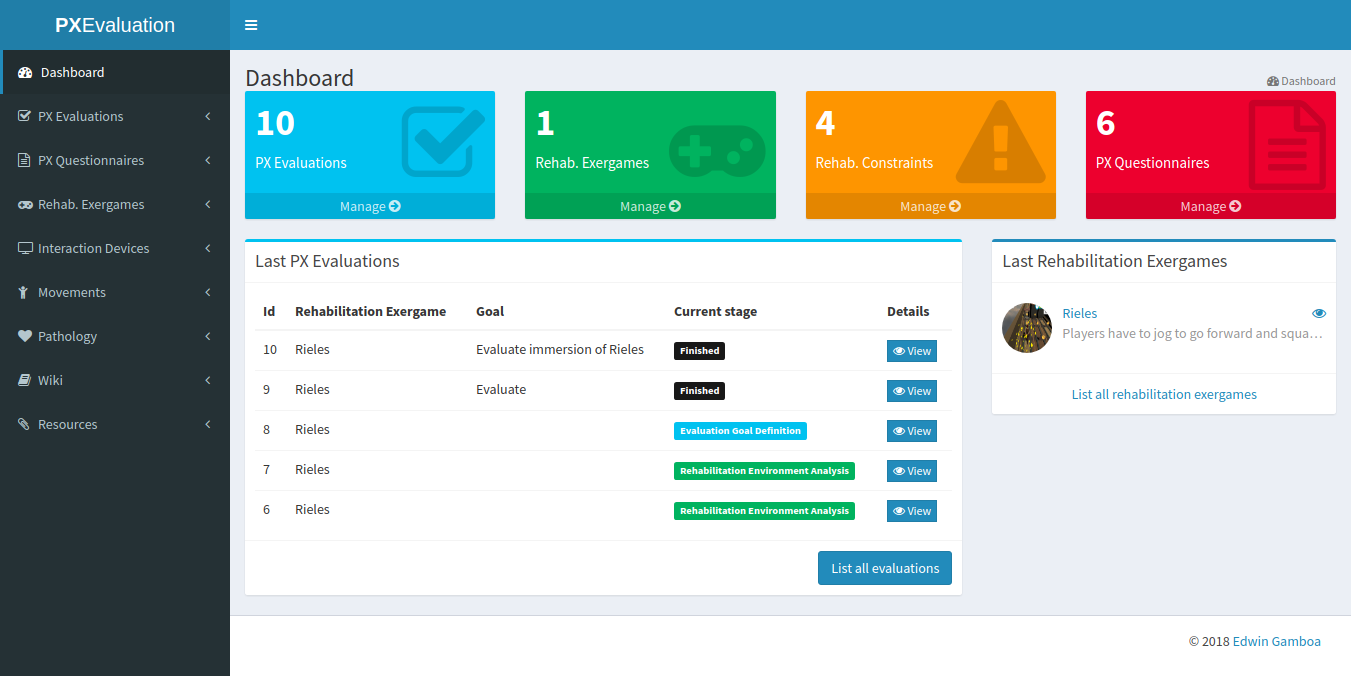
\includegraphics[width=\linewidth]{gfx/app/dashboardApp}} \quad
\caption{Dashboard of the \ac{PX} evaluation application}\label{fig:dashboardApp}
\end{figure}

\begin{figure}[bth]
\myfloatalign
{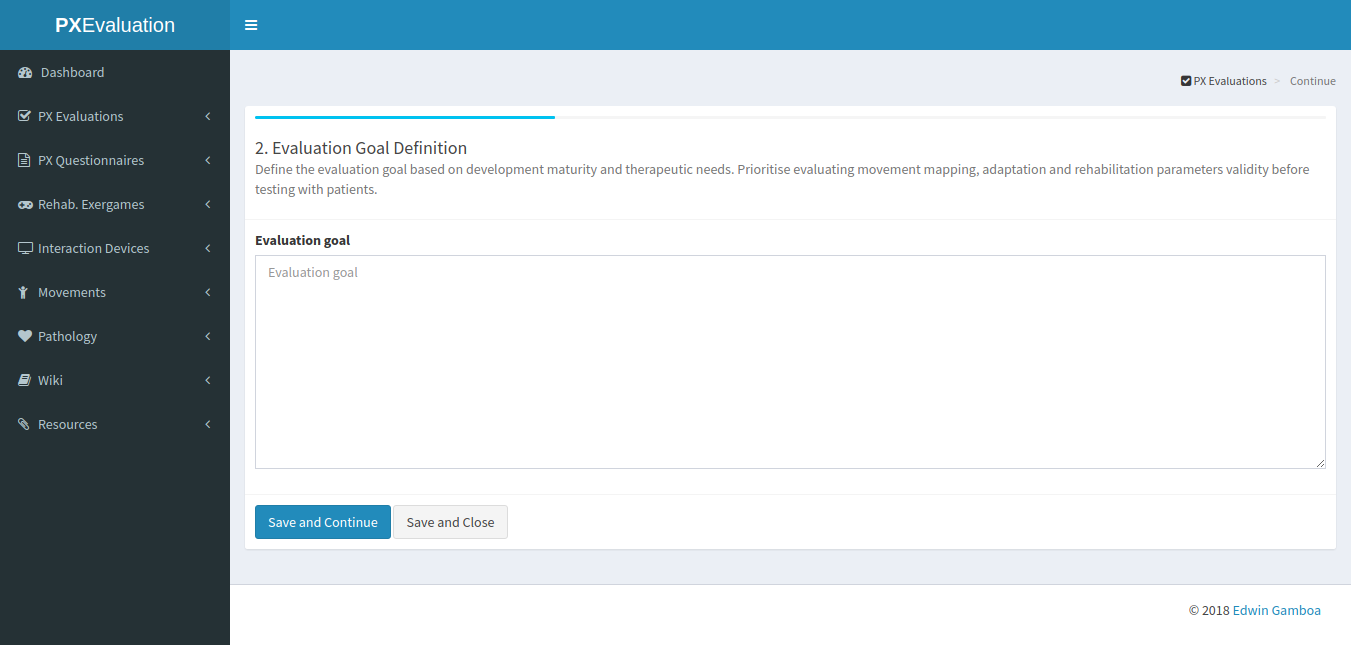
\includegraphics[width=\linewidth]{gfx/app/evaluationApp1}} \quad
\caption{Register view of an evaluation at the \ac{PX} evaluation application}\label{fig:evaluationApp1}
\end{figure}

\begin{figure}[bth]
\myfloatalign
{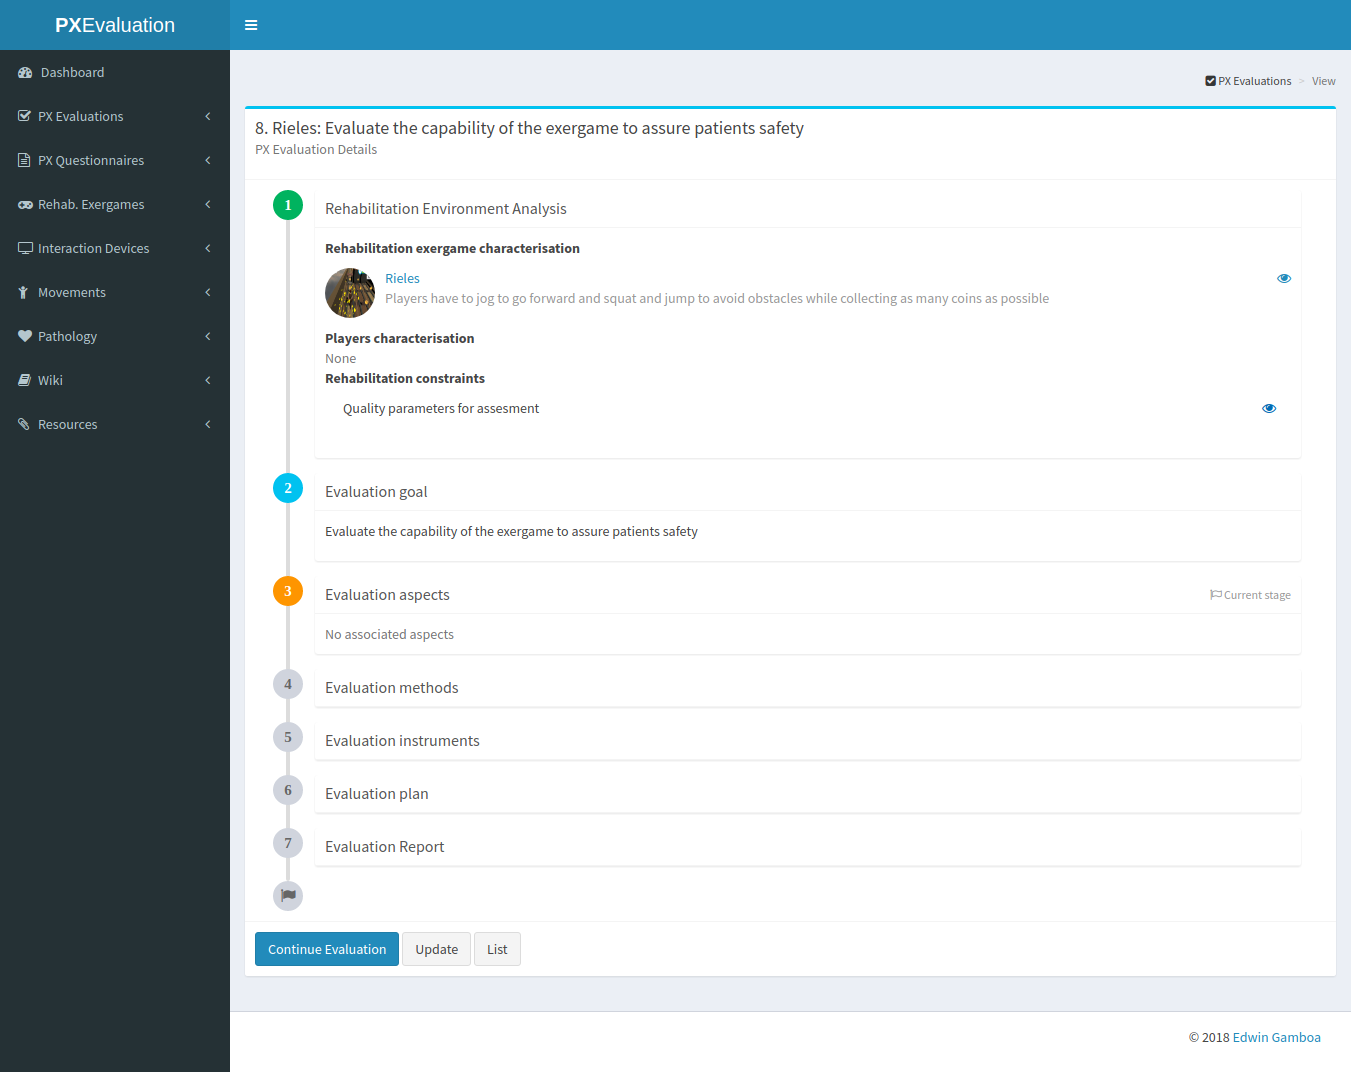
\includegraphics[width=\linewidth]{gfx/app/evaluationApp2}} \quad
\caption{Detail view of an evaluation at the \ac{PX} evaluation application}\label{fig:evaluationApp2}
\end{figure}


\begin{figure}[bth]
\myfloatalign
{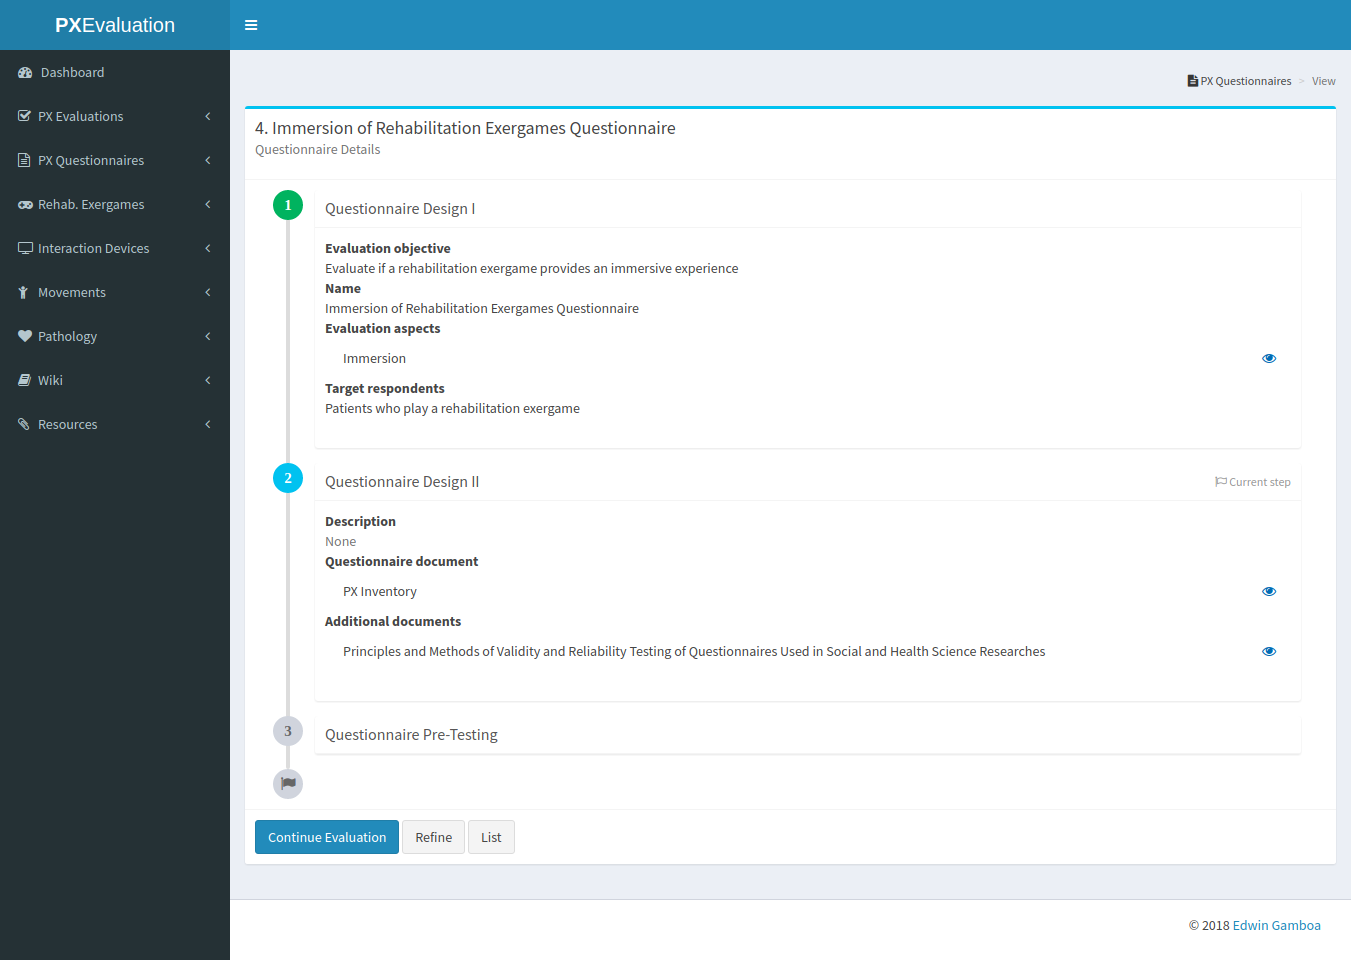
\includegraphics[width=\linewidth]{gfx/app/standardApp}} \quad
\caption{Detail view of a standard being developed at the \ac{PX} evaluation application}\label{fig:standardApp}
\end{figure}

\begin{figure}[bth]
\myfloatalign
{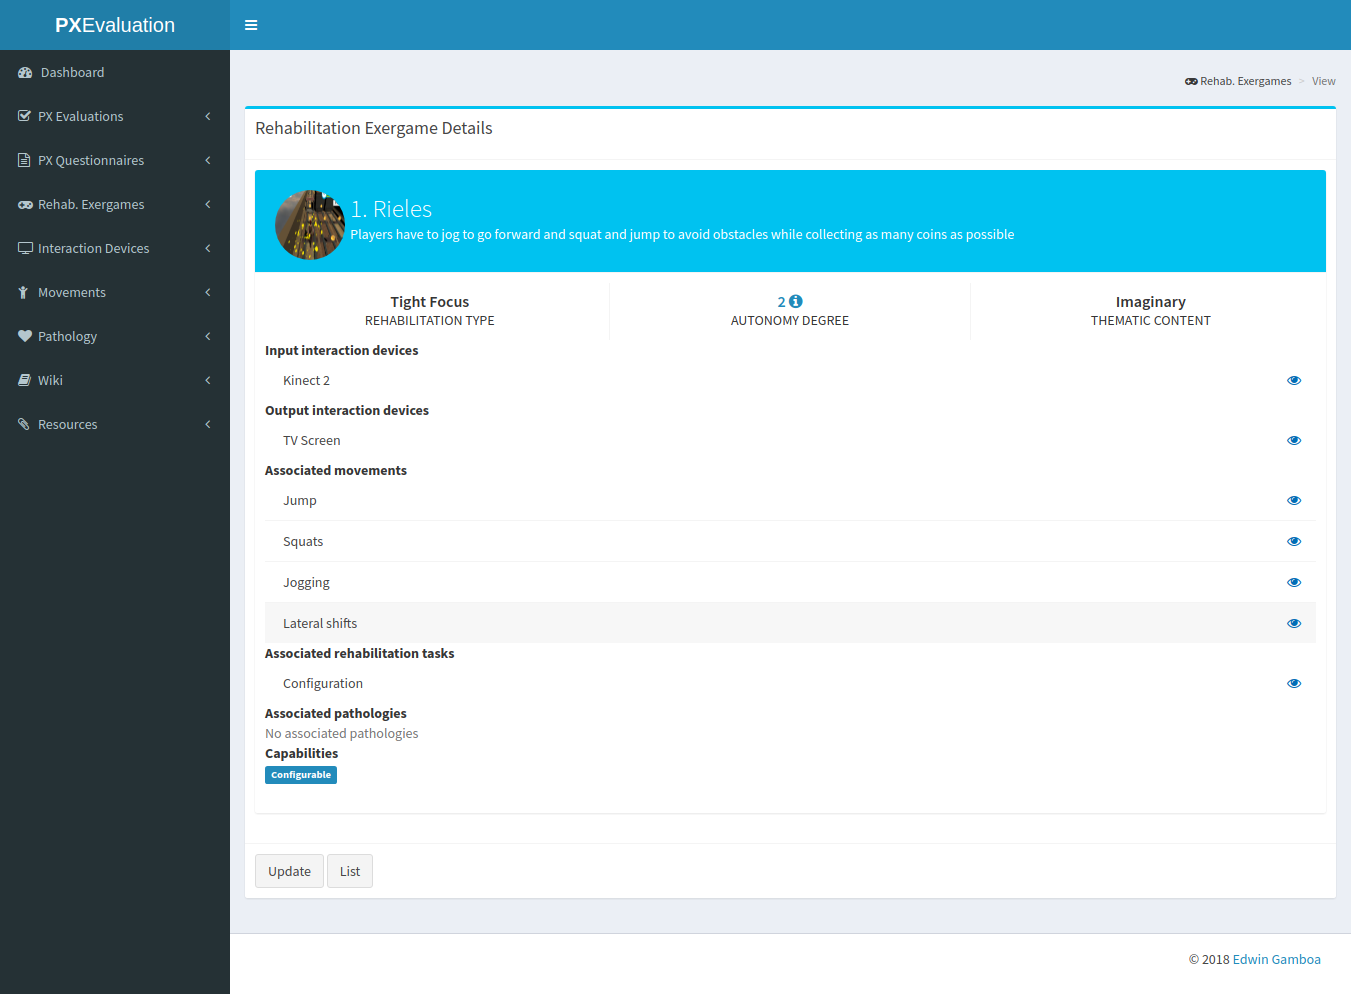
\includegraphics[width=\linewidth]{gfx/app/characterisingApp}} \quad
\caption{Detail view of a \ac{PREG} characterisation at the \ac{PX} evaluation application}\label{fig:characterisingApp}
\end{figure}

\section{Conclusion}
In this chapter, we presented a methodology for evaluating PX in \acp{PREG}. Our proposal is based on the model presented on \autoref{ch:model}; highlighting crucial aspects to be evaluated before, during and after interaction between a patient, a context and a \ac{PREG} occurs. Since the methodology is based on a \ac{PX} model for \acp{PREG}, it allows performing evaluations that meet the constraints that the rehabilitation environment may impose. It requires evaluators to characterise \acp{PREG} considering its therapeutic goal, to define users profile considering its characteristics as patients and analysing the involved rehabilitation environment. Thus, our approach differs from other evaluations in which \acp{PREG}s are evaluated considering only motivation, enjoyment or usability \autocite{Brokaw2015,Burke2009,Cameirao2010,jansen2013serious,Ni2014}.

The proposed methodology is intended to be used iteratively to perform a comprehensive evaluation. However, it was built based on a model designed using a qualitative approach, thereby limiting its generalisation. Thus, we still need to use the methodology extensively to identify gaps and additional constraints that should be considered. This process would allow us to validate the relevance of the highlighted stages in real use cases.

Finally, the proposed methodology may be extended or adapted to other domains in which entertainment is not the main goal. In that case, the domain constraints should be identified to define a set of relevant aspects, methods and instruments to be employed during \ac{PX} evaluation.

\chapter{Standard Proposal: Guidance on the Development of PX Questionnaires}
\label{ch:questionnaire}

% Introduction (Explain and contextualise objective)
% 
One of the most employed \ac{PX} evaluation methods is using questionnaires. A questionnaire allows collecting self-reported data from players before, during or after interacting with a game. Although there are some standardised \ac{PX} questionnaires \autocite{denisova_convergence_2016,VandenAbeele2016,Calvillo-Gamez2015,Brockmyer2009,Poels2008,DeKort2007,Vorderer2004}, the most common approach is to develop ad-hoc questionnaires to evaluate \ac{PX} \autocite{Yanez-Gomez2017}. In the case of rehabilitation exergames, we identified constraints that can represent challenges when evaluating \ac{PX} in \autoref{ch:characterising}. Existing standardised questionnaires may be useful to evaluate aspects such as enjoyment, immersion, presence and flow. However, evaluating \ac{PX} in rehabilitation exergames may require developing questionnaires that address those constraints.

Nevertheless, there is no a standardised process to develop a questionnaire for \ac{PX} or even \ac{UX} evaluation. Existing questionnaires have been developed following different approaches. In this chapter, we present the design of a standard proposal to develop questionnaires to evaluate \ac{PX}. Our proposal is based on 22 documents that we reviewed to identify and integrate recommendations, guides and adopted practices for developing questionnaires. Also, we studied the current status of standardisation in the \ac{UX} field to identify how to develop a standard properly; i.e., following guidelines of a relevant standardisation organisation. Then, we integrated our findings into a standard process.

% -----------------------------------------------
\section{Standardisation} % Standardisation -----------------------------------------------
\label{sec:standardisation}
To the extent of the author's knowledge, a standard to develop questionnaires to evaluate rehabilitation exergames is not defined. However, there are usability and \ac{UX} standards which are a relevant reference for the process of standardising \ac{PX}. Below, we present a review of \ac{UX} standards.

\textcite{Ran2015} present a summary of standards and standardisation organisations related to usability and \ac{UX} (See \autoref{fig:standardisation_orgs}). The most influential international organisations are \ac{ISO}, \ac{IEC} and \ac{ITU} \autocite{Ran2015}. While, \ac{CEN} and  \ac{ETSI} are relevant European standardisation organisations.

\ac{ISO} formulated the \textit{ISO 9241} standards, which are considered general and broad and have had the highest impact \autocite{Ran2015}. The most relevant parts of this standard are \textit{ISO 9241:11} \autocite{iso9241:11} and \textit{ISO 9241:210} \autocite{iso9241:210}. The first one, guides users on the usability of hardware and software systems; and the second one, guides the design of human-centred interactive systems and introduces the concept of \ac{UX}.

Meanwhile, the TC 122 working group from \ac{CEN} organisation works on ergonomics standardisation for designing work systems and work environments. A list of standards published by this working group can be found at its website\footnote{https://standards.cen.eu}. The \ac{IEC} technical committee ISO/IEC JTC 1/SC 35 works on user interfaces standardisation for \ac{ICT}. A list of publications from this committee can be accessed from its website\footnote{http://www.iec.ch}.

The other two organisations formulate \ac{UX} and usability standards in specific fields. First, \ac{ETSI} has formulated several standards in human factors and accessibility of \ac{ICT}, including fixed, mobile, radio, broadcast and internet technologies. These standards can be accessed at the organisation's website\footnote{http://www.etsi.org/technologies-clusters/technologies/human-factors-accessibility}. Meanwhile, \ac{ITU} and specifically the study group 12 works on standards for performance, \ac{QoE} and \ac{QoS} of next-generation networks\footnote{https://www.itu.int/en/ITU-T/studygroups/2017-2020/12/Pages/default.aspx}.

\begin{figure}[htb]
\myfloatalign
{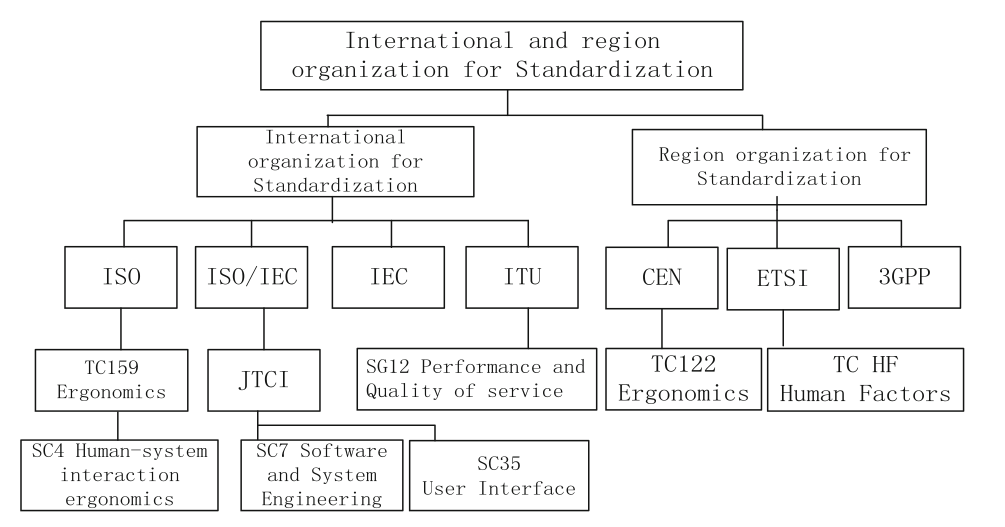
\includegraphics[width=\linewidth]{gfx/standard/standardisation_orgs}} \quad
\caption[Standardisation organisations related to usability and \ac{UX}]{Standardisation organisations related to usability and \ac{UX} \autocite{Ran2015}}\label{fig:standardisation_orgs}
\end{figure}

Most of these standards are not publicly available. From the above organisations only \ac{ETSI} provide copies of its standards directly at its website.

\subsection{ISO 9241:210}
As mentioned above, ISO 9241 Ergonomics of human-system interaction standards are the most relevant in the field of \ac{UX} \autocite{Ran2015}. From these standards, the ISO 9241:210 \autocite{iso9241:210} is of high relevance since it introduces the concept of \ac{UX}. According to this standard, \ac{UX} can be defined as "person's perceptions and responses resulting from the use and/or anticipated use of a product, system or service". The standard also mentions three notes about this definition. The first note highlights that \ac{UX} includes the experience before, during and after use. The second note explains that \ac{UX} also is affected by characteristics of the interactive system, the users internal and physical state and the context of use. The third note explains that \ac{UX} can be considered and evaluated as usability when it is interpreted from the perspective of users' personal goals.

Additionally to \ac{UX}, this standard presents other definitions including accessibility, context of use, usability, usability attributes, interactive system and human centred design. Moreover, it describes some benefits of adopting human-centred design; e.g., \ac{UX} improving, productivity increasing, ease of understanding, cost reduce among others.

The standard also describes six principles of human-centred design:

\begin{enumerate}
    \item the design is based upon an explicit understanding of users, tasks and environments
    \item users are involved throughout design and development
    \item the design is driven and refined by user-centred evaluation
    \item the process is iterative
    \item the design addresses the whole \ac{UX}
    \item the design team includes multidisciplinary skills and perspectives
\end{enumerate}

The third principle indicates that evaluation must be carried out to gather feedback from users. This evaluation may reduce the risk of producing a system which does not meet user needs. Other, principles may also apply to evaluation; i.e., users involvement, whole \ac{UX}, iterative process and multidisciplinary skills are also desirable for \ac{UX} evaluation.

Furthermore, the document details the activities of the human-centred design process, which are presented in \autoref{tab:huma_centred_activities} and detailed in \autocite{iso25060}.

\begin{table}[htb]
\caption[Activities of the human-centred design process]{Activities of the human-centred design process}
\label{tab:huma_centred_activities}
\begin{center}
\begin{tabularx}{.9\textwidth}{Xp{5.5cm}}
\toprule
%----------------------
\spacedlowsmallcaps{Activities} 
& \spacedlowsmallcaps{Outputs}
\\ \midrule
%----------------------
Understand and specify the context of use
&
Context of use description
\\
\midrule
%----------------------
\multirow{3}{*}{Specify the user requirements}
&
Context of use specification
\\&
User needs description
\\&
User requirements specification
\\\midrule
%----------------------
\multirow{3}{5.5cm}{Produce design solutions to meet these requirements}
&
User interaction specification
\\&
User interface specification
\\&
Implemented user interface
\\\midrule
%----------------------
\multirow{3}{5.5cm}{Evaluate the designs against requirements}
&
Evaluation results
\\&
Conformance test results
\\&
Long-term monitoring results
\\\midrule
%----------------------
\bottomrule
\end{tabularx}
\end{center}
\end{table}

The last human centred-design activity is \textit{Evaluating the design}. According to this standard, evaluators should evaluate a design concept from the user's perspective. That would allow evaluators to gain a better understanding of users' needs is gained. However, the direct participation of users is not completely necessary; i.e, evaluators can employ inspection-based evaluation. A human-centred evaluation allows collecting new information about users, gathering the strengths and weaknesses of the design solution, assessing user requirements achievement and establishing baselines to compare different designs.

According to the standard, a user-centred evaluation should involve allocating resources for early and late evaluation, planning, carrying sufficient testing out, analysing results, proposing solutions and communicating those solutions to the design team. Evaluations can be carried out along the whole project life cycle.

The standard presents two approaches for user-centred evaluation: 

\begin{itemize}
    \item \emph{User-based evaluation}: requires the participation of users. At early stages, it allows testing design concepts against the real world. Also, evaluators can collect feedback about the acceptability of a design.
    At later stages, evaluators can assess the achievement of usability objectives in the context of use.
    \item \emph{Inspection-based evaluation}: involves the participation of usability experts who play the role of users to evaluate the system. Evaluators use their knowledge, guidelines, heuristics and standards among others. This kind of evaluation is cost-effective; however, it relies on the evaluators' skills and knowledge.
\end{itemize}

User-centred evaluation methods and guidance on how and when to use them are presented in \autocite{iso16982}.

%-----------------------------------
\section{Materials and methods} % Materials -----------------------------------
\label{sec:mats_mets_sta}

We conducted a literature review to identify recommendations and current practices in the development of questionnaires. We reviewed 21 documents, 14 documents reported the development of \ac{UX} or \ac{PX} questionnaires and the remaining 7 corresponded to guides for developing and composing questionnaires (See \autoref{tab:rev_docs_sta}). We identified the stages, activities, methods and best practices employed or suggested in each document. Then, we classified and grouped findings to compose a comprehensive process to develop questionnaires for \ac{PX} evaluation. The conducted process is illustrated in \autoref{fig:methods_sta}.

\begin{table}[htp]
\caption{Reviewed documents to develop the standard proposal}
\label{tab:rev_docs_sta}
%\myfloatalign
\begin{tabularx}{\textwidth}{p{3cm}X}
\toprule
%----------------------
\spacedlowsmallcaps{Type} 
& \spacedlowsmallcaps{Document Title}
\\ 
\midrule
%----------------------
\multirow{7}{3cm}{\ac{PX} Questionnaire} &
Assessing the Core Elements of the Gaming Experience \autocite{Calvillo-Gamez2015}
\\
%\cline{2-2}
%----------------------
& FUGA-the fun of gaming: measuring the human experience of media enjoyment \autocite{Poels2008}
\\
%\cline{2-2}
%----------------------
& The development of the Game Engagement Questionnaire: A measure of engagement in video game-playing \autocite{Brockmyer2009}
\\
%\cline{2-2}
%----------------------
& MEC spatial presence questionnaire (MEC-SPQ): Short documentation and instructions for application \autocite{Vorderer2004}
\\
%\cline{2-2}
%----------------------
& Digital games as social presence technology: Development of the Social Presence in Gaming Questionnaire (SPGQ) \autocite{DeKort2007}
\\
%\cline{2-2}
%----------------------
& Rapid assessment of game experiences in public settings \autocite{Moser2012}
\\
%\cline{2-2}
%----------------------
& The convergence of player experience questionnaires \autocite{Denisova2016}
\\
\midrule
%----------------------
\multirow{2}{3cm}{\ac{PX} Scale} &
EGameFlow: A scale to measure learners’ enjoyment of e-learning games \autocite{Fu2009}
\\
%\cline{2-2}
%----------------------
& Design and preliminary validation of the Player Experience Inventory \autocite{VandenAbeele2016}
\\
\midrule
%----------------------
\multirow{2}{3cm}{\ac{UX} Questionnaire} &
Construction and evaluation of a User Experience Questionnaire \autocite{Laugwitz2008}
\\
%\cline{2-2}
%----------------------
& AttrakDiff: Ein Fragebogen zur Messung wahrgenommener hedonischer und pragmatischer Qualität \autocite{Hassenzahl2003}
\\
\midrule
%----------------------
\multirow{2}{3cm}{Usability Questionnaire} &
Measuring usability with the use questionnaire \autocite{lund2001measuring}
\\
%\cline{2-2}
%----------------------
& Development of an instrument measuring user satisfaction of the Human-computer Interface \autocite{Chin1988}
\\
\midrule
%----------------------
Usability scale
&
SUS-A quick and dirty usability scale \autocite{Brooke1996}
\\
\midrule
%----------------------
\multirow{7}{3cm}{Guide} &
Administering, analysing, and reporting your questionnaire \autocite{Boynton2004}
\\
%\cline{2-2}
%----------------------
& Reaching beyond the white middle classes \autocite{Boynton2004b}
\\
%\cline{2-2}
%----------------------
& Selecting, designing, and developing your questionnaire \autocite{Boynton2004c}
\\
%\cline{2-2}
%----------------------
& A step-by-step guide to developing effective questionnaires and survey procedures for program evaluation \& research \autocite{Diem}
\\
%\cline{2-2}
%----------------------
& Questionnaire design \autocite{Crawford1997}
\\
%\cline{2-2}
%----------------------
& Tips for developing and testing questionnaires/instruments \autocite{Radhakrishna2007}
\\
%\cline{2-2}
%----------------------
& Question and questionnaire design \autocite{Krosnick2009}
\\
\midrule
%----------------------
\bottomrule
\end{tabularx}
\end{table}

\begin{figure}[htb]
\myfloatalign
{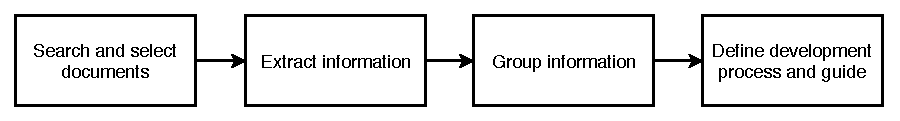
\includegraphics[width=\linewidth]{gfx/standard/MethodStad}} \quad
\caption{Process conducted to develop the questionnaires standard proposal}\label{fig:methods_sta}
\end{figure}

The standard proposal was composed following the principles and rules for the structure and drafting of documents by \ac{ISO}, \ac{IEC} \autocite{ISO2016}.

%-----------------------------------
\section{Standard Proposal: Guidance on Questionnaires Development} % Results -----------------------------------
% Requirement: shall, shall not. 
% Recommendation: should, should not
% Permission: may, need not
% Possibility and capability: can, cannot
% External constraint Verbal: must

\label{sec:sta_proposal}

\subsection{Introduction}
A questionnaire is a data collection method that allows gathering information from people. A reliable and valid questionnaire can be used over time by different interviewers or researchers, involving different samples of the target audience. As a consequence, one can compare the results of different studies objectively.

This document aims to provide guidance on how to develop a valid and reliable questionnaire to those responsible for evaluating \ac{PX} aspects using questionnaires.

\subsection{Scope}

This document specifies a process for developing valid and reliable questionnaires for evaluating \ac{PX} aspects. Also, it includes a guide for formulating questions. It is intended to be used by those responsible for developing questionnaires to evaluate \ac{PX} aspects collecting information from a specific audience. The process encompasses the preparation, design and pre-testing of a questionnaire. It does not provide detailed coverage of specific techniques and methods associated questionnaire development activities.

Presentation, format, layout and styles of questionnaires are outside the scope of this document.

\subsection{Normative references}
There are no normative references in this document.

\subsection{Terms and definitions}
For the purposes of this document, the following terms and definitions apply.

\subsubsection{Questionnaire}
A data collection method that helps gather information about knowledge, attitudes, opinions, behaviours, facts and other information \cite{Radhakrishna2007}.

\subsubsection{Standardised questionnaire}
A questionnaire that is written and administered precisely. That is, all respondents are asked the same questions, and their responses are registered uniformly \cite{Boynton2004c}.

\subsubsection{Researcher}
A person who develops a questionnaire.

\subsubsection{Interviewer}
A person who administers a questionnaire.

\subsubsection{Respondent}
A person who answers a questionnaire.

\subsubsection{Valid questionnaire}
A questionnaire that measures what it is intended to measure \cite{Boynton2004c}.

\subsubsection{Reliable questionnaire}
A questionnaire that produces consistent results for repeated samples and when administered by different interviewers \cite{Boynton2004c}.

\subsubsection{Closed question}
A question that requires respondents to select an answer from a set of choices \cite{Krosnick2009}.

\subsubsection{Screening question}
A question that may have follow-up questions depending on how respondents answer it \cite{Krosnick2009}.

\subsection{Symbols and abbreviated terms}
\begin{acronym}[UML]
\acro{PX}{Player Experience}
\acro{UX}{User Experience}
\acro{HCI}{Human Computer Interaction}
\acro{AI}{Artificial Intelligence}
\end{acronym}

\subsection{Questionnaire development process}

\autoref{fig_quesDevProcess} presents the process of questionnaire development. It comprises three main activities and involves three decisions. Throughout the process, researchers will develop or select a valid and reliable questionnaire for evaluating one or more \ac{PX} aspects. The process is detailed below.

\begin{figure}[htb]
\myfloatalign
{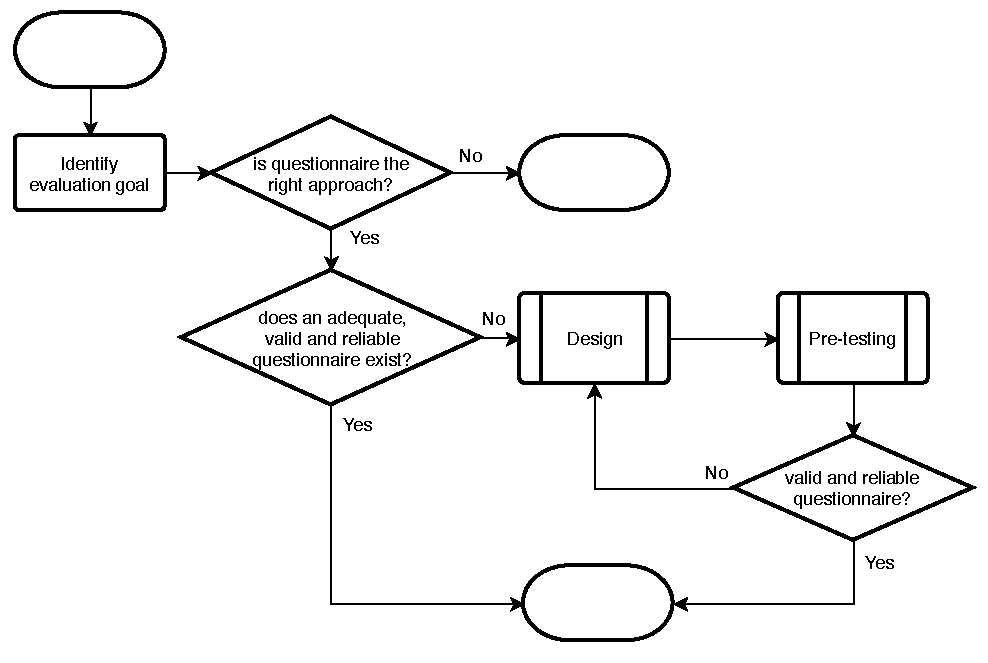
\includegraphics[width=0.9\linewidth]{gfx/standard/quesDevProcess}} \quad
\caption{Questionnaire development process}\label{fig_quesDevProcess}
\end{figure}

\subsubsection{Identify evaluation goal}
In this stage, researchers determine the information they need to know and the reasons to know it. This may result in the identification of an \emph{evaluation goal} \cite{Diem,Radhakrishna2007,Crawford1997}. Nevertheless, defining an evaluation is not straightforward since it involves exploratory research. That includes consulting experts or collecting data from people directly related to the problem itself; e.g. by performing a focus group, reviewing literature \cite{Crawford1997}.

\subsubsection{Is questionnaire the right approach?}
Researchers determine whether using a questionnaire is the right approach to achieve the evaluation goal \cite{Boynton2004c}. Depending on the goal, other data collection methods may be more appropriate than questionnaires; e.g. observation, video recording, interview and existing data analysis among others. A multi-method approach may also be convenient \cite{Boynton2004c,Krosnick2009}, in such a case, researchers should define a more specific goal for the questionnaire.

If a questionnaire is not appropriate to meet the evaluation goal, the development process finishes since no questionnaire is to be selected or designed.

\subsubsection{Does an adequate, valid and reliable questionnaire exists?}
Researchers determine whether they can employ an existing questionnaire instead of designing a new one \cite{Boynton2004c}. If researchers have conducted an exploratory research in the first stage, they might have an initial idea of how similar studies were carried out and what instruments were employed. Otherwise, they should conduct an additional exploration to identify existing questionnaires, which could be employed to achieve research objectives. If any questionnaire is available, researchers should identify whether it is reliable and valid. Note they shall prefer standardised questionnaires over other alternatives \cite{Boynton2004c}.

If researchers identify an appropriate, valid and reliable questionnaire; they can use it and this process finishes. Otherwise, researchers should continue with the design stage.

\subsubsection{Design}
Researchers decide on questions, wording, format and layout among others. The main output of this stage is a version of the questionnaire and accompanying documents. This step comprises a whole sub-process, which is described in \autoref{sec:ques_design}.

\subsubsection{Pre-testing}
Researchers test the questionnaire they designed during the last stage. Pre-testing should be planned, and the data should be collected, processed, analysed and reported. Researchers should establish the validity and reliability of the designed questionnaire. This step comprises a whole process, which is described in \autoref{sec:ques_pretesting}.

\subsubsection{Validity and reliability check}
Researchers determine whether the designed questionnaire is valid and reliable enough. If so, the process is finished successfully. Otherwise, researches should return to the design stage and iterate until they achieve the desired reliability and validity.

\subsection{Questionnaire design}
\label{sec:ques_design}
Designing a questionnaire is a respondent centred process. It requires researchers to determine the aspects to be studied and define the target respondents. Then, researchers shall produce questions that allow studying those aspects. Those questions shall be understood and answered accurately by target respondents. To achieve that, researchers should take care of wording, format, number and order of questions. \autoref{fig_quesDesignProcess} shows an overview of the process and further details are provided below.

\begin{figure}[htb]
\myfloatalign
{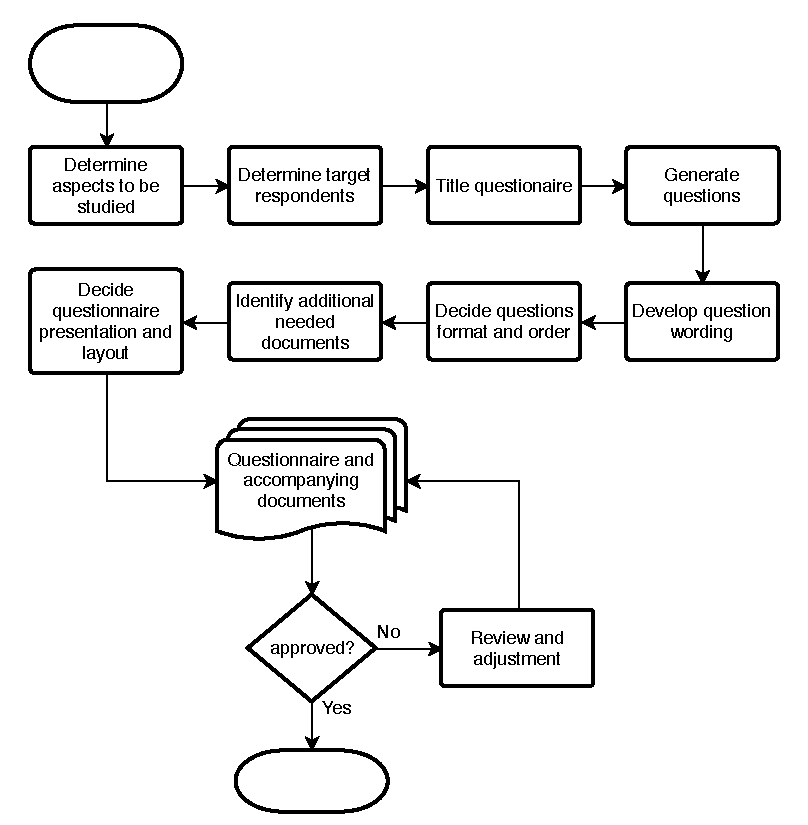
\includegraphics[width=0.9\linewidth]{gfx/standard/quesDesignProcess}} \quad
\caption[Questionnaire design process]{Questionnaire design process}\label{fig_quesDesignProcess}
\end{figure}

\subsubsection{Determine aspects to be studied} 
Researchers shall define which \ac{PX} aspects they will study to achieve the defined evaluation goal. Examples of \ac{PX} aspects include motivation, effectiveness, ease of use, attractiveness.

\subsubsection{Determine target respondents}
Researches shall define the appropriate population to be asked. This step also includes identifying characteristics of the target respondents that should be considered during the design process, e.g., age, education level, familiarity with questionnaires, cultural bias or language barriers \cite{Diem,Crawford1997}. Also, researchers should not exclude disadvantaged groups to avoid biases and generalisation errors due to misunderstandings or ambiguity \cite{Boynton2004b}.

Determining the correct target respondents is important since researchers will make generalisations upon their responses. That is, target respondents represent the population to whom the results of the questionnaire would apply \cite{Crawford1997,Diem}. Consequently, researchers should employ research techniques when they do not know the target audience.

\subsubsection{Title questionnaire}
Researchers shall choose a title that informs respondents about the sought evaluation goal \cite{Diem}.

\subsubsection{Generate questions}
Researchers shall generate as many questions as possible for each aspect to be evaluated. At this stage, details such as wording are not important. The generated questions shall meet the evaluation goal and allow studying the aspects  selected \cite{Crawford1997,Radhakrishna2007}.

\subsubsection{Filter questions}
Researchers shall only include questions that allow achieving the evaluation goal and studying each selected aspect. Nevertheless, researchers may include a few redundant questions to gain respondents' involvement and motivation \cite{Crawford1997}.

\subsubsection{Develop question wording and format}
Researchers shall produce questions that can be understood by respondents to collect complete, unbiased and accurate answers. Also, the questionnaires shall be easy to administer for interviewers. To aim that, researchers may include explanations and definitions for each question. They shall produce brief questions to keep respondents interested \cite{Crawford1997}. 
A question can be open, closed or closed with an open response option \cite{Crawford1997}. Researchers should select a consistent format for the whole questionnaire. 
Regarding closed questions, researchers should use scales that have precise and clear answer categories, provide needed information and are uniform and appropriate for respondents  \cite{Diem,Krosnick2009}. Researches shall make sure that questions match the selected scale \cite{Diem}. When researchers use a rating scale, they shall make it progressive and select answer categories that represent respondents' opinion meaningfully. Researchers shall not select a low or a high number of scale points. Five to seven points are recommended \cite{Krosnick2009}.

Additional question formats include statements with tick box categories, visual analogue scales and symbols \cite{Boynton2004c}.

\subsubsection{Decide questions order}
Researchers shall order questions logically to promote understating and motivation \cite{Diem,Krosnick2009}. They should:
\begin{enumerate}
    \item Put the most important questions at the beginning of the questionnaire \cite{Diem}. Those questions may be connected to the questionnaire purpose and impose minimal burden \cite{Krosnick2009}.
    
    \item Avoid putting difficult questions at the beginning to avoid respondents to get demotivated \cite{Krosnick2009}.
    
    \item Avoid putting difficult questions at the end to avoid wrong answers due to fatigue \cite{Krosnick2009}.
    
    \item Avoid putting screening questions at the beginning since respondents may answer inaccurately to avoid answering remaining questions \cite{Krosnick2009}.
    
    \item Put demographic and sensitive questions at the end to avoid threatening respondents. Also, researchers shall provide information about the reasons to collect such data to gain respondents' trust \cite{Boynton2004b,Krosnick2009}.
    
    \item Group related questions \cite{Krosnick2009}.
    
    \item Avoid questions to be weighted due to order. Researchers should analyse questions context when possible. Otherwise, they may randomise order \cite{Krosnick2009}.
\end{enumerate}

\subsubsection{Decide questionnaire presentation and layout}
Researchers should create questionnaires that look professional since presentation has a significant effect on the quality and quantity of the obtained data \cite{Diem,Crawford1997}. To achieve that, researchers should use simple and clear formats, use booklets, use space and font adequately, use colour coding for different questionnaire versions and keep the questionnaire as short as possible \cite{Crawford1997}.

\subsubsection{Identify additional needed documents}
Researchers may include accompanying documents for clarity and motivation purposes. Additional documents include cover or appreciation letters, guides for respondents or interviewers, documents providing details about the study, e.g., time and place \cite{Diem,Crawford1997,Boynton2004b}.

\subsubsection{Questionnaire and accompanying documents}
Researchers shall assemble the questionnaire and accompanying documents into a single deliverable. They should check and review the questionnaire, e.g., using checklists available online\footnote{\url{http://www.bmj.com/content/328/7451/1312?panels_ajax_tab_tab=jnl_bmj_tab_related_art&panels_ajax_tab_trigger=related\#c}}.

\subsubsection{Approval}
Researchers shall determine if the questionnaire needs to be approved before it can be administered. Approval source may be internal or external to researchers organisation \cite{Diem}.

\subsubsection{Review and adjustment}
If the questionnaire requires approval but it was not approved, researchers shall review and adjust the questionnaire until reaching approval.

\subsection{Pre-testing}
\label{sec:ques_pretesting}
Pre-testing or piloting process allows researchers to know whether a questionnaire would achieve desired results \cite{Crawford1997}, identifying problems associated to it. Pre-testing a questionnaire allows evaluating questions wording, order and relevance. After pre-testing, researchers will know if a questionnaire is complete, understandable and does not cause discomfort to respondents \cite{Boynton2004}. Pre-testing is also an opportunity to determine if interviewers are well trained to administer a questionnaire \cite{Crawford1997}. \autoref{fig_quesPretesting} presents an overview of this process.

\begin{figure}[htb]
\myfloatalign
{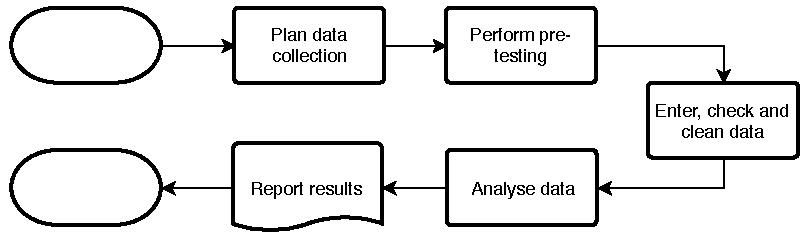
\includegraphics[width=0.9\linewidth]{gfx/standard/quesPretesting}} \quad
\caption[Questionnaire pre-testing process]{Questionnaire pre-testing process}\label{fig_quesPretesting}
\end{figure}

\subsubsection{Plan pre-testing}
Pre-testing a questionnaire requires researchers to plan well in advance to collect high-quality data. Planning a pre-testing involves deciding:

\begin{enumerate}
    \item \emph{Target respondents participation}: researchers shall decide if respondents participation is needed or available. If participants are needed, they shall represent target respondents \cite{Krosnick2009,Boynton2004}.
    Researchers shall use sampling techniques to select participants \cite{Boynton2004c,Diem,Radhakrishna2007}. They can find a set of techniques and details on how to use them online\footnote{\url{https://www.bmj.com/content/328/7451/1312?panels_ajax_tab_tab=jnl_bmj_tab_related_art&panels_ajax_tab_trigger=related\#d}}.
    Regarding the number of participants, researchers should prefer fewer answers with good quality, than a high number of answers with inaccurate or incomplete responses \cite{Boynton2004}. On the other hand, if respondents participation is not required, researchers shall invite experts to test and evaluate the questionnaire.
    
    \item \emph{Collection methods and procedures}: when researchers decide not to include respondents, pre-testing should be conducted using methods such as expert review, statistical modelling or \ac{AI} techniques. On the other hand, if target respondents participation is required, pre-testing should be conducted in similar conditions to a real questionnaire administering session \cite{Krosnick2009}. In that case, researchers shall choose the data collection method based on target respondents needs and preferences, which have been identified during the design stage. Also, researchers shall consider available resources and the evaluation goal \cite{Boynton2004}.
    Data collection methods include personal interviews, focus groups, mail questionnaires, web based questionnaires, telephone interviews, post questionnaires and interviewer guided \cite{Crawford1997,Diem,Boynton2004}. Researchers can find pros and cons of each method online\footnote{\url{https://www.bmj.com/content/328/7452/1372?panels_ajax_tab_tab=jnl_bmj_tab_related_art&panels_ajax_tab_trigger=related\#3}}.
    Researchers shall be aware of data protection laws and internal codes, e.g., from researchers' or respondent's organisations \cite{Boynton2004}.
    
    \item \emph{Interviewers training}: people who conduct the pre-testing shall be trained or supervised. They should be prepared for answering and managing respondents' questions and unexpected reactions \cite{Boynton2004b}.
\end{enumerate}

\subsubsection{Perform pre-testing}
During pre-testing researchers should observe, record or take notes on important issues such as misunderstood, surprising or confusing questions, the time required by respondents to complete the questionnaire and respondents' reactions \cite{Boynton2004}. Researchers shall assure privacy, anonymity and non-threatening surroundings. Additionally, when interviewers are helping respondents to fill in the questionnaires, they should avoid inflexions on voices, facial expressions or gestures to avoid biases \cite{Boynton2004b}.
Finally, researchers should thank respondents for their participation \cite{Diem}.

\subsubsection{Enter, check and clean data}
Researchers shall enter, check and clean data to be analysed. They shall agree on and understand the tools to be used for this stage. This process should be carried out as soon as data is collected to avoid having to process a large amount of data  \cite{Boynton2004}.

\subsubsection{Analyse data}
Researches shall select an analysis method based on the collected data \cite{Boynton2004,Diem}. A set of analysis methods are listed online\footnote{\url{https://www.bmj.com/content/328/7452/1372?panels_ajax_tab_tab=jnl_bmj_tab_related_art&panels_ajax_tab_trigger=related\#4}}. At this stage, researchers shall establish the questionnaire reliability using measures such as Test-Retest or Internal Consistency Measures \cite{Radhakrishna2007,Diem}. Finally, they should establish questionnaire validity using a panel of experts or field test. Also, they should use readability tests like the Fog Index or Flesch Reading Ease \cite{Radhakrishna2007}.

\subsubsection{Report results}
Researchers shall filter relevant data to be reported \cite{Boynton2004,Diem} and how they will present the results. A set of recommendations about how to present data is presented in \cite{Boynton2004}. Researchers shall focus report on presenting and discussing the main findings. Also, they shall report reliability and validity indicating how these measures were established \cite{Radhakrishna2007}.

\subsection{Guide for formulating questions}
\label{sec:questions_guide}
When composing questionnaire questions, the following recommendations should be considered:

\begin{enumerate}
    \item Researchers should, if possible, involve representatives of target respondents in the design process of a questionnaire \cite{Boynton2004b}.
    
    \item Researchers should include explanations or examples when asking about abstract things \cite{Boynton2004b,Crawford1997}. However, specific and concrete wording is preferred over abstract wording \cite{Krosnick2009}.
    
    \item Researchers should use simple vocabulary that respondents can understand. They should consider that some words have different meanings in different contexts \cite{Boynton2004b,Diem,Krosnick2009}.
    
    \item Researchers should avoid complex routing for screening questions since that reduce respondents motivation and lead to indiscriminate answers \cite{Boynton2004b}.
    
    \item Researchers should pay careful attention to the demographic data that they intend to collect. They should avoid asking sensitive and threatening data. Pre-testing questionnaires allow identifying this issue \cite{Boynton2004b}.
    
    \item Researchers should, if possible, use official translators or translation services when developing questionnaires in more than one language \cite{Boynton2004b}.
    
    \item Researchers should avoid excluding disadvantaged groups of respondents to avoid biases, misunderstandings or ambiguity\cite{Boynton2004b}.
    
    \item Researchers should use specific adverbs instead of frequently, regularly, commonly, usually and hardly among others \cite{Boynton2004c,Krosnick2009}.
    
    \item Researchers should offer enough answer options when using closed questions to avoid respondents' frustration \cite{Boynton2004c}. Also, answer options should be mutually exclusive \cite{Krosnick2009}.
    
    \item Researchers should carefully plan when using open questions. They should consider time, skills and resources required for respondents to answer and for researchers to analyse the questionnaire \cite{Boynton2004c}.
    
    \item Researchers should avoid starting questionnaires with threatening questions \cite{Diem}.
    
    \item Researchers should include simple instructions \cite{Diem}.
    
    \item Researchers should be as brief as possible \cite{Diem}.
    
    \item Researchers should ask one question at a time \cite{Diem,Krosnick2009}.
    
    \item Researchers should include easy to answer questions at the beginning of a questionnaire \cite{Crawford1997,Krosnick2009}. Initial questions should also address the questionnaire topic directly \cite{Krosnick2009}.
    
    \item Researchers should order questions in a way that one leads naturally to the other. Additionally, researchers should be group questions on the same topic \cite{Crawford1997,Krosnick2009}.
    
    \item Researchers should include sensitive questions at the end of a questionnaire to avoid respondents cutting off before important information is collected \cite{Crawford1997,Krosnick2009}.
    
    \item Researchers should allow filtering questions to avoid that respondents answer questions that do not apply to them \cite{Krosnick2009}.
    
    \item Researchers should include a balanced number of answer options when using rating scales. Five to seven options have been proved to lead to reliable and valid questionnaires \cite{Krosnick2009}.
    
    \item Researchers should label points of rating scales. They should divide points into approximately equal units \cite{Krosnick2009}.
    
    \item Researchers should assure anonymity to avoid social desirability response bias \cite{Krosnick2009}.
    
    \item Researchers should avoid burdening respondents. To achieve this, they should reduce the reference period, use yes/no questions instead of all that apply questions and avoid making respondents perform computations that researchers can do \cite{Krosnick2009}.
\end{enumerate}

% -----------------------------------------------
\section{Validation} % Validation -----------------------------------------------
We started a submission process for our standard proposal at \ac{ICONTEC}, the Colombian Member Body of \ac{ISO} since it can submit a new work item proposal to the ISO/TC159/SC4 Ergonomics of human-system interaction technical committee. We have become a member of the Technical Committee 20 of \c{ICONTEC} (\textit{Comit\'e T\'ecnico de Normalizaci\'on (CTN) 20 Ergonom\'ia)}, we should participate in some meetings before they can consider our proposal for submission.

% -----------------------------------------------
%\section{Discussion} % Discussion -----------------------------------------------
%Reiterate the Research Problem/State the Major Findings: 
%Explain the Meaning of the Findings and Why They are Important: expected? unexpected? (explain these especially). unusual or unanticipated patterns or trends that emerged from your results and explain their meaning in relation to the research problem. 
%Relate the Findings to Similar Studies: compare your results with other studies or use the studies to support a claim.
%Consider Alternative Explanations of the Findings: a claim for how the results can be applied more generally. For example, describing lessons learned, proposing recommendations that can help improve a situation, or highlighting best practices.
%End: concise summary of the principal implications of the findings regardless of significance. Why you believe the findings and conclusions of your study are important and how they support broader knowledge or understanding of the research problem. This can be followed by any recommendations for further research. A more general claim or possible conclusion arising from the results. E.g. new research questions.

% -----------------------------------------------
\section{Conclusion} % Conclusion -----------------------------------------------
\label{sec:conclusion_2}
We presented a standard proposal for developing questionnaires to evaluate \ac{PX} aspects. Our proposal integrates practices that have been adopted to develop well-known \ac{UX} and \ac{PX} questionnaires and recommendations from questionnaire development experts. We identified the most influential standardisation organisation (i.e., \ac{ISO}) and its Colombian Body Member (\c{ICONTEC}) to start a submission process for our standard proposal. Our may contribution is related to standardising the process of developing reliable a valid questionnaires for evaluating \ac{PX} aspects, thereby making possible to compare and use results from different questionnaires uniformly.

\chapter{Evaluating PX in Playtherapy rehabilitation exergames}
\label{ch:playtherapy}
The goal of this project was to propose a comprehensive model to evaluate \acp{PREG} considering the entertaining and the rehabilitation purposes. In \autoref{ch:model}, we proposed a model that meets that requirement; and in \autoref{ch:methodology}, we presented a methodology to evaluate \ac{PX} in rehabilitation exergames based on that model. In this chapter, we present a study case in which we used the proposed model to evaluate \ac{PX} in a \ac{PREG}. The \ac{PREG} is called Playtherapy and is being developed by the Multimedia and Computer Vision research group from \textit{Universidad del Valle} and the Evaristo Garc\'ia University Hospital from Cali Colombia.

The remaining of this chapter is organised as follows. First, we present Playtherapy and its development environment. Then, we describe the \ac{PX} evaluation that we have conducted. Finally, we conclude the chapter presenting the main contributions and limitations of the evaluation.

To evaluate \ac{PX} in Playtherapy we employed the methodology presented in \autoref{ch:model}. \autoref{tab:conducted_evaluations} presents a summary of the evaluations conducted to evaluate Playtherapy's exergames.



\section{Antecedents}
% Game in dev
% Sessions: aspects, methods, instruments, participants
We conducted three semi-structured interviews with three physiotherapists (2 female, 1 male) from the Evaristo Garc\'ia University Hospital. We obtained informed consents from the participants verbally. The interviews were audio recorded. The goal of the interviews is to collect information about the \emph{context} where they will use Playtherapy, their expectations regarding its use and the \emph{patients' profile}. Furthermore, the game system was characterised identifying Playtherapy's architecture and using the approach presented in \autoref{sec:characterising}. Additionally, two members of the development team, a physiotherapy student and a programmer, evaluated each mini-game using the \ac{RITE} method. A summary of the evaluation process is presented in \autoref{tab:antecedents_evaluations} and detailed in the following sections.

\begin{table}[bth]
\myfloatalign
\caption{Conducted evaluation sessions to evaluate antecedents of Playtherapy}
\resizebox{\linewidth}{!}{
\begin{tabularx}{1.3\textwidth}{m{1.5cm}m{4.5cm}XXXm{1.8cm}}
%----------------------
\toprule
\spacedlowsmallcaps{Layer}
& \spacedlowsmallcaps{Goal}
& \spacedlowsmallcaps{Aspects}
& \spacedlowsmallcaps{Methods}
& \spacedlowsmallcaps{Participants}
& \spacedlowsmallcaps{Sessions} \\\midrule
Context
& Identify the profile of physiotherapists from the hospital and the hospitals' regulations required to perform an evaluation
& Rehabilitation environment
& \multirow{2}{*}{Interview}
& \multirow{2}{2cm}{3 physiotherapists}
& \multirow{2}{*}{2} \\\cline{1-3}
Player/ Patient
& Identify a general profile of patients from the hospital
& Player profile &  &  &  \\\midrule
\multirow{3}{*}{Game}
& Characterise Playtherapy's mini-games
& Characteristics
& Inspection, characterisation \autoref{sec:characterising}
& 1 \ac{PX} evaluator
& - \\\cline{2-6}
& \multirow{2}{4.5cm}{Assess whether Playtherapy meets the requirements to be used by patients}
& \multirow{2}{3cm}{Configuration capability, Tutorial quality, Movement support}
& \ac{RITE}
& 1 physiotherapy student, 1 programmer
& 10 \\\cline{4-6}
&  &  & Question asking protocol
& 1 physiotherapist, 1 physiatrist
& 5\\ \midrule
\bottomrule
\end{tabularx}}
\label{tab:antecedents_evaluations}
\end{table}

\subsection{Context}
% interviews were conducted: three participants, verbal consent, 
% Data analysed using thematic content analysis
% results: personas were developed
As described in \autoref{sec:rel_among_dimension}, the context layer comprises the cultural parameters and the rehabilitation environment associated with the use of Playtherapy. To collect data about context, we use the following guiding questions for the conducted semi-structured interviews:

\begin{enumerate}
    \item \item What activities occur during physical therapy sessions?
    \item How can a \ac{PREG} be used as part of physical therapy?
    \item How do you expect to use \ac{PREG}?
    \item How do you think \acp{PREG} should assist patients?
    \item What kind of devices and software do you use on a regular basis?
\end{enumerate}

\subsubsection{Cultural parameters}
Regarding \emph{cultural parameters}, the physiotherapists have not used \acp{PREG} in the hospital; thus, we did not identify local game communities. Some of the physiotherapists have used commercial exergames for their entertainment and outside the hospital. Only the academic community would represent an environment to share experiences and find relevant information. 

\subsubsection{Institution}
Regarding the \emph{rehabilitation environment}, the physiotherapists expressed that a typical rehabilitation therapy starts with an evaluation or diagnosis session, which will serve as input to establish rehabilitation goals and a treatment plan. A diagnosis session is performed according to the \ac{APTA} and the \ac{ICF} and may involve assessing aspects such as motion range, functional Independence, oxygen saturation, \ac{HR}, fine motor skill, balance, resistance and strength. During a rehabilitation treatment, physiotherapists perform re-evaluations periodically to assess patients progress and adapt treatment plan accordingly (e.g. by including new exercises or physical instruments). Patients' progress is tracked using forms established by the hospital. That confirms the relevance of the therapy tasks presented in \autoref{sub:def_rehab_therapy}; i.e., personalisation, supervision and assessment since they allow physiotherapists to determine whether a patient can use Playtherapy or not.

A therapy session takes one hour and comprises warm-up, cool-down and main therapeutic exercises, which are planned by a physiotherapist. In the first session, physiotherapists instruct patients to maintain a correct posture, avoid unsafe movements and take adequate precautions during exercises. Also, physiotherapists should explain and supervise each exercise execution specifying how to perform it correctly. At the end of each session, physiotherapists give feedback to patients and register important observations on a form. Moreover, auxiliary staff assist physiotherapists supervising and instructing patients. The decision to include a Playtherapy mini-game in a therapy session relies mainly on physiotherapists' criteria based on evaluation and re-evaluation results.

Playtherapy would be used in the Physical medicine and rehabilitation unit of the hospital. It has different facilities including a walk training area, a gym, a physical agents area, children area and adults area. Some of these places are usually crowded; thus, the location to use Playtherapy should be selected carefully. The unit is trying to provide two rooms to be used exclusively for playing Playtherapy.

Also, we identified internal regulations and constraints which are important to conduct an evaluation successfully. We need the approval of the head of the physical medicine and rehabilitation unit and the ethical committee of the hospital. A physiotherapist will be in charge of internal processes and logistics such as location, date, time, hospital participants and health instruments when needed. We should provide and coordinate the technical logistics.  When an evaluation requires patients' participation, we should inform the physiotherapist at least four weeks in advance to arrange an appointment; otherwise, two weeks in advance would be enough. Finally, for long-term evaluations involving patients, we need the approval of the technical committee of the physical medicine and rehabilitation unit.

\subsubsection{Physiotherapists}
About \emph{physiotherapists profile and expectations}, they expressed that they feel confident using technologies since they are used to interact with smart-phones, computers and tablets. One of them has played exergames with Kinect One and Nintendo Wii. Another physiotherapist considered herself a casual player. The physiotherapists remarked that they are in charge of deciding what a patient can do in a therapy session since they are responsible for patients' safety. The physiotherapists expect Playtherapy to add variety and dynamism to the therapies they conduct, aid patients to reach the rehabilitation goals, motivate patients to perform the expected rehabilitation movements while reaching game goals, provide patients with information about goals, performance and progress. Moreover, they require Playtherapy to be an assisting tool that can be configurable to patients' needs and preferences (to assure patients' safety) and offer the possibility to work on particular joints and movements. They do not want Playtherapy to increase their workload. \autoref{fig:physio_personas} presents the two persona models that we built based on collected information.

\begin{figure}[bth]
\centering
 \subfloat[Physiotherapist with average IT mastery]{
   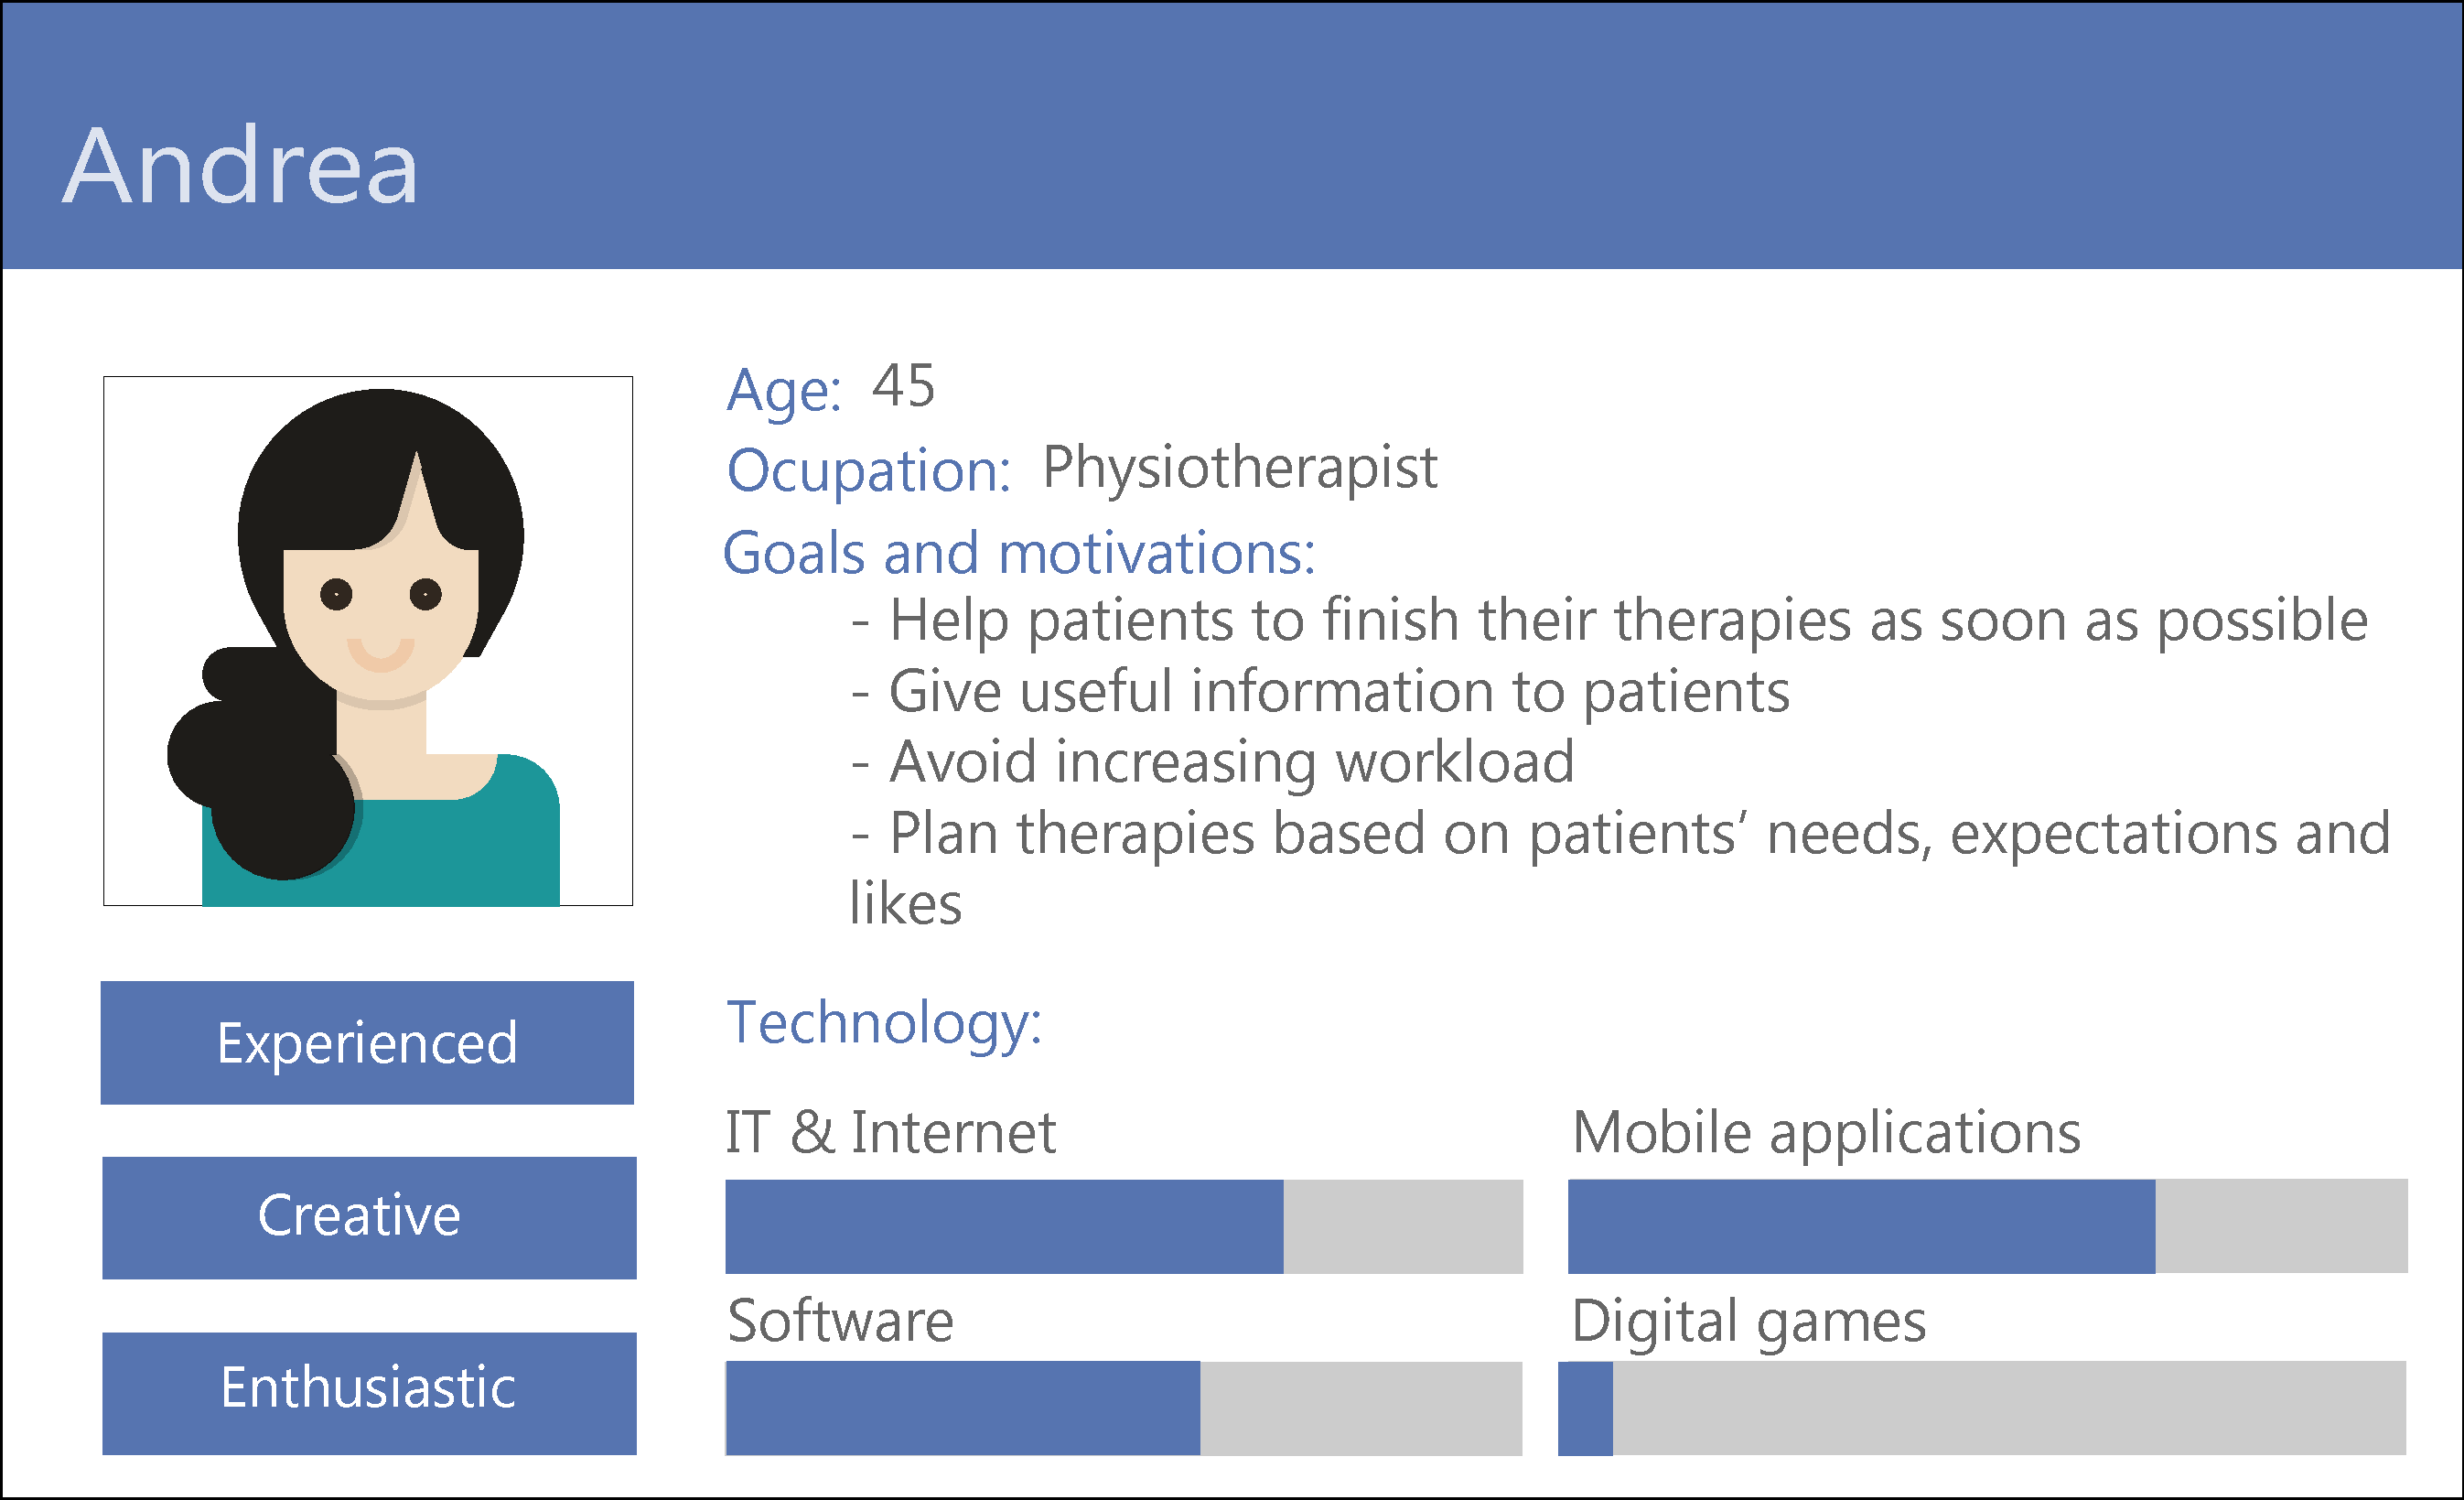
\includegraphics[width=0.48\linewidth, frame]{gfx/playtherapy/personaPhyAndrea}
   \label{fig:personaPhyAndrea}
 }
 \subfloat[Physiotherapist who sympathises with games]{
   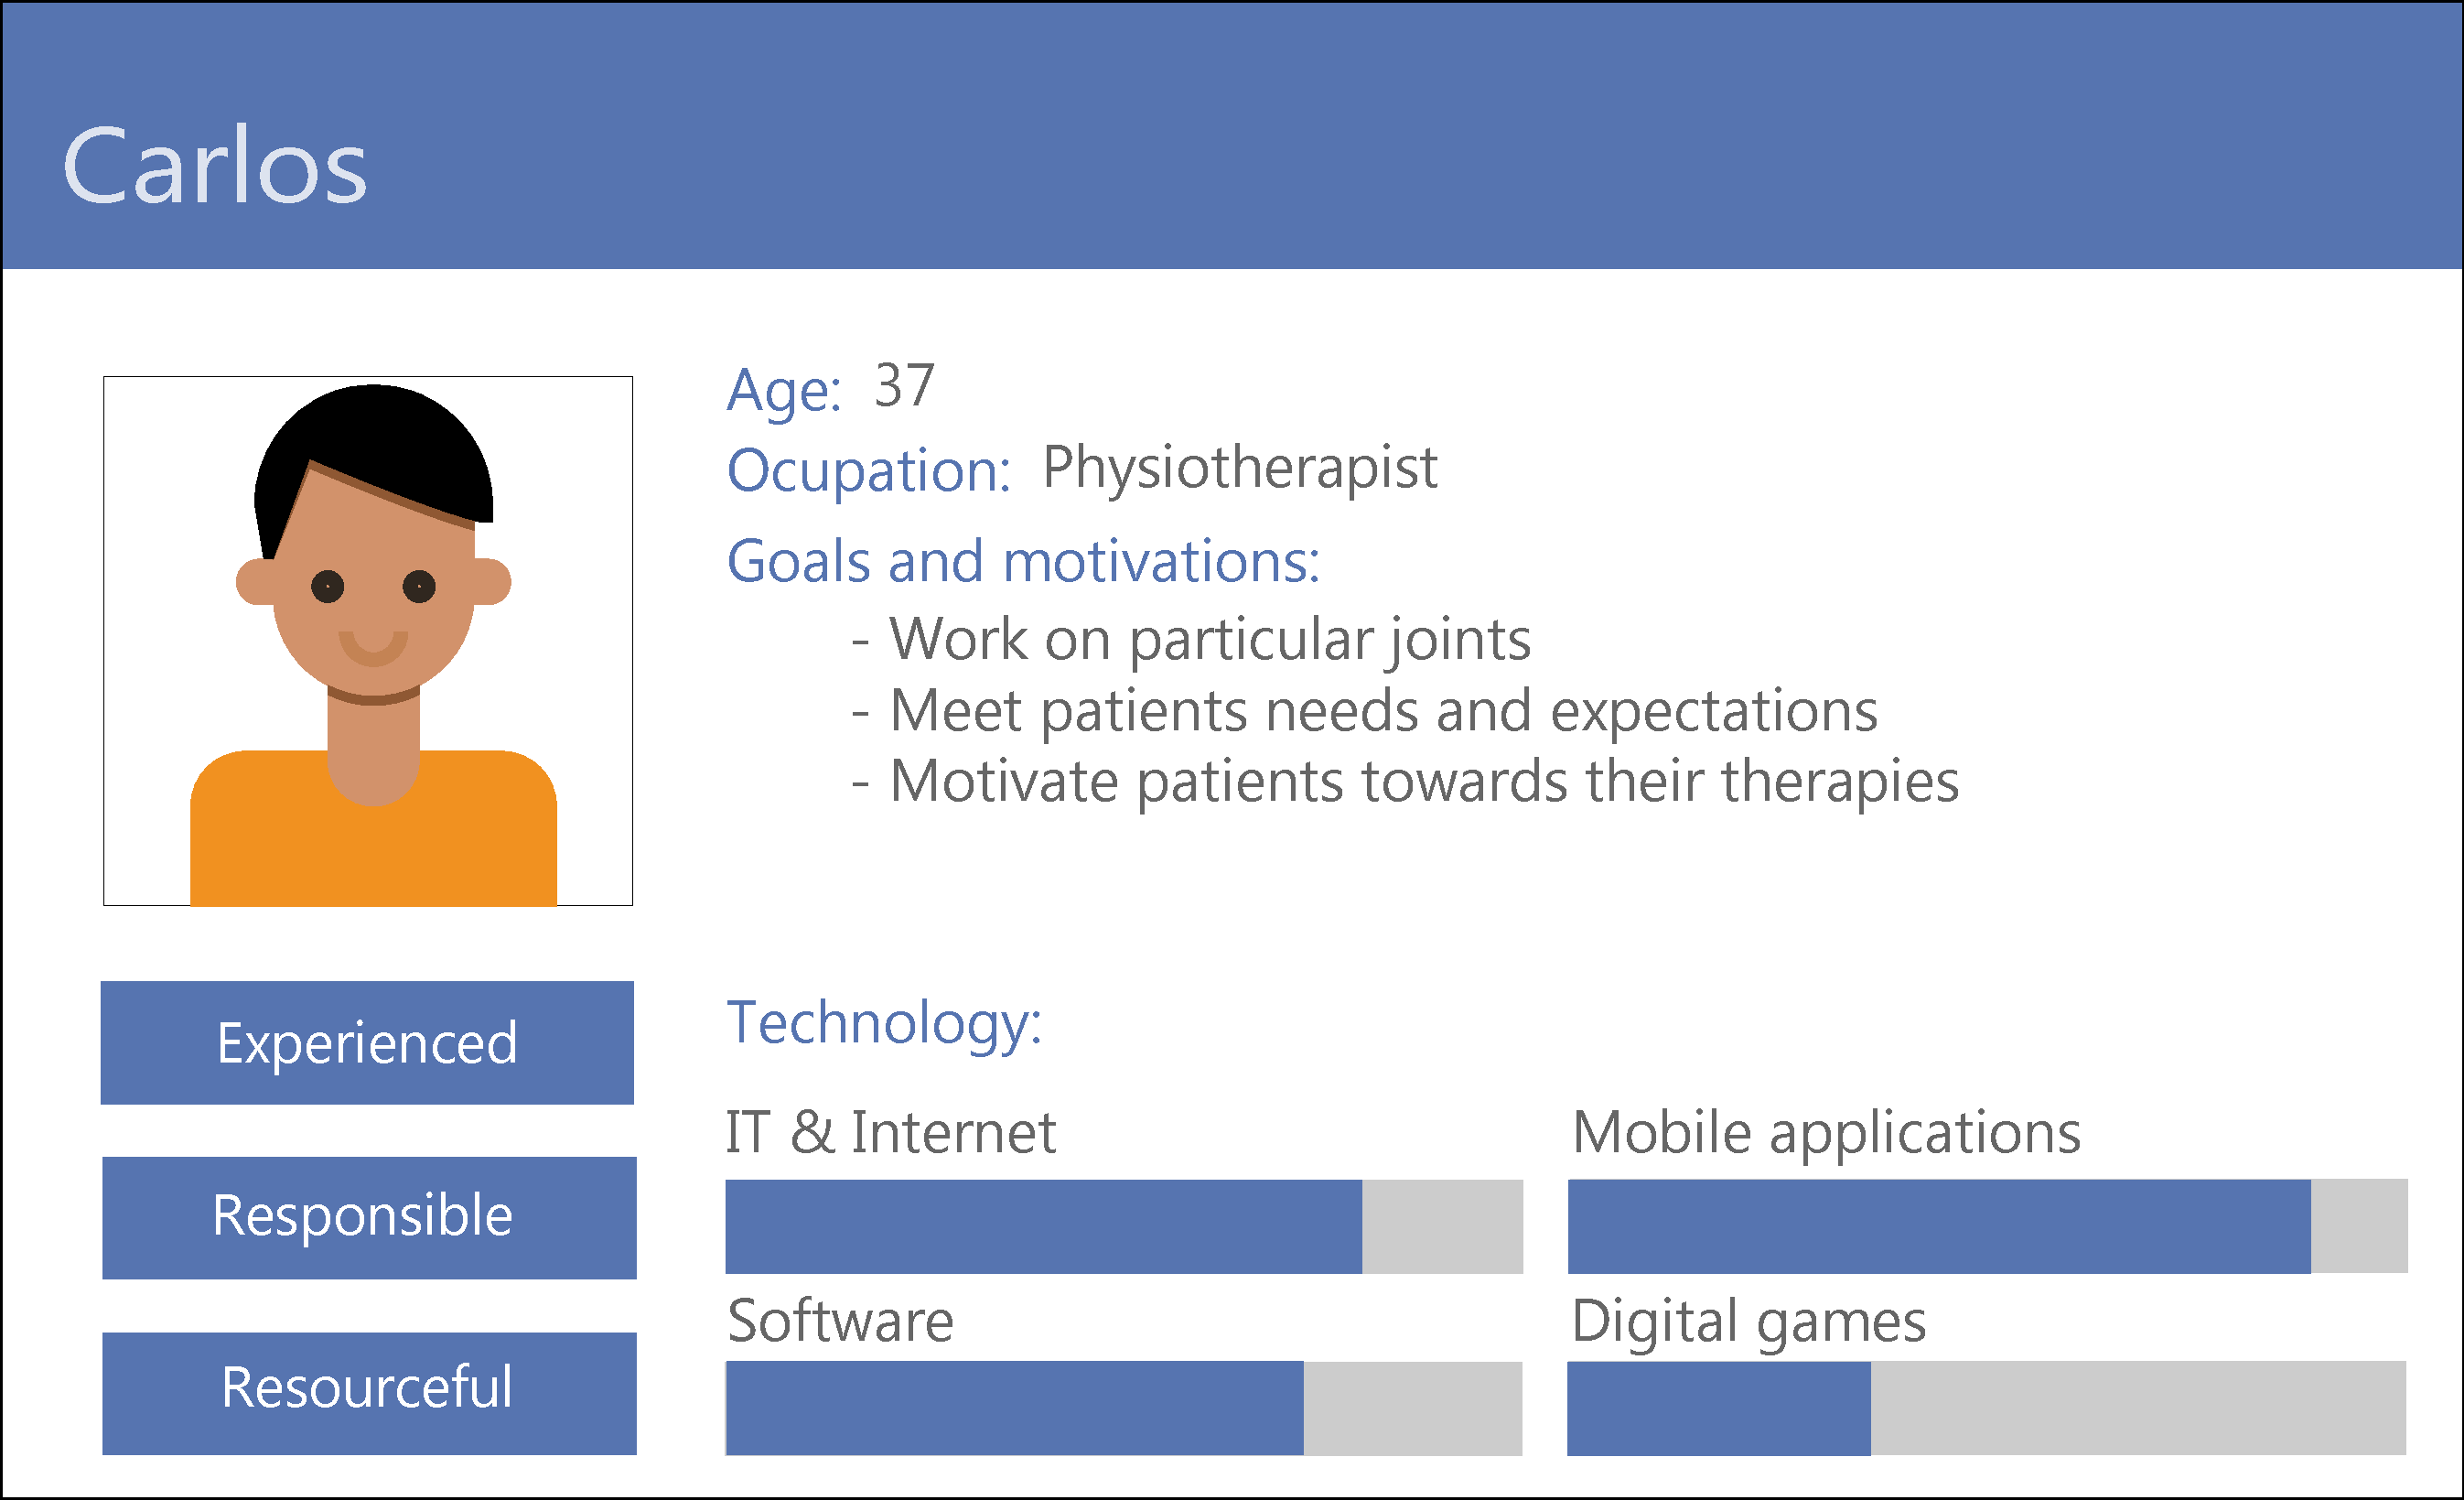
\includegraphics[width=0.48\linewidth, frame]{gfx/playtherapy/personaPhyCarlos}
   \label{fig:personaPhyCarlos}
}
\caption{Physiotherapists' persona models}
\label{fig:physio_personas}
\end{figure}

\subsection{Player/Patient}
Following the proposed model \autoref{sec:rel_among_dimension}, we identified characteristics, motivations and expectations of patients of the hospital to build Persona models. We use the following guiding questions to collect the data:

\begin{enumerate}
    \item What kind of patients participate in physical therapy?
    \item How is patients' motivation towards physical therapy?
    \item What factors affect patients' motivation towards physical therapy?
\end{enumerate}


Specific information about game activity, health status and previous experiences of players is collected before conducting any evaluation of \emph{Interaction} that involves patients (See \autoref{sec:interaction_eval}).

\subsubsection{Demographic characteristics}
The physiotherapists expressed that patients who require physical therapies have musculoskeletal, cardiopulmonary and neuromuscular pathologies including lower and upper limbs fracture or traumas, cerebral palsy, joint dislocation and stroke. In the case of Playtherapy, it would be targeted at musculoskeletal patients since they require active exercises. Chronic patients are those who have a very limited range of motion of one or more joints.

Regarding age, the physical medicine and rehabilitation unit of the hospital treats children from five to twelve years old. However, most patients are over the age of eleven. Also, young patients (thirteen to seventeen years old), young adult patients (seventeen to thirty-five years old), adults (thirty-six to sixty years old) and elderly patients (older than sixty years old) are treated.

Most children who are treated at the unit are attending primary school. Most young patients have finished primary school and attend secondary school, though, some of them quit before finishing it since they start working. Most young adults have finished secondary school or are finishing it. Some of them have completed a technical career. Most adult and elderly patients have finished at most primary school. Few of the adults have finished secondary school.

Most children who are treated at the unit are attending primary school. Most young patients have finished primary school and attend secondary school, though, some of them quit before finishing it since they start working. Most young adults have finished secondary school or are finishing it. Some of them have completed a technical career. Most adult and elderly patients have at most finished primary school. Few of the adults have finished secondary school.

The unit treats female and male children proportionally. Young and young adult patients are mainly male. Meanwhile, adult and elderly patients are mostly female. All patients belong to the lower or working classes; i.e., one, two and three Colombian social strata.

Regarding the work with patients, the physiotherapists commented that children and young patients are willing to work during the therapy sessions and understand what they should do easily. Young adults and adults do not like reading and prefer visual aids. Finally, physiotherapists should monitor elderly patients closely since they have comprehension difficulties and get confused with the instructions easily.

\subsubsection{Motivations and expectations}

% Las mayor expectativa del paciente es finalizar la terapia rápido

% Los pacientes se demotivan por la repetición y monotonía de los ejercicios
% El paciente quiere saber cuánto dura su tratamiento de recuperación

%Si tiene una razón externa, ej: trabajar, poder reintegrarse a la vidad diaria: vestirse, peinarse, ...; para lograr el objetivo terapeutico, entonces puede estar motivado

% Si el pacietne es juciosos y continúa los ejercicios en casa puede tener mejor progreso -> motivación

% Adultos tempranos y mayores, son más grupales que individuales. Clase de pilates, clase de yoga, usar un deporte inclusivo

% Con los niños se trabaja con juegos
% El ínteres de los pacientes es una recuperación pronta
% Los niños debe ser más interactivos, dinámicos. Con juego
% Niños juegos, ayudas didácitca, visual
%Disposición en niños es alta. Con ellos es díficl lograr atención. El mismo ejercicio los aburre. Se debe ser recursivo, quieren hacer muchas cosas. 

% Jóvenes, coversar sobre temas de ínteres, usando ayudas didacticas ayuda a motivarlos
% Jóvenes son dispuestos, se prestan muchoa las recomendaciones hechas por los fisioterapeutas
% Disposición en jóvenes, adultos temprano y medio dispuesto colaboradores.

% Disposición mayores: la edad es una limitación, puede ser díficil realizar un ejercicio
% Disposición mayores: la edad es una limitación, puede ser díficil realizar un ejercicio

% Los pacientes pueden mejorar su disposición si el fisioterapeuta agrega variedad a la terapia, ej: incrementando dificultad. inluyendo nuevos elementos. Depende de la creatividad del fisio

\subsection{Game system}

\subsubsection{General characteristics}
Playtherapy is a collection of mini \acp{PREG} whose purpose is to increase patients' motivation towards completing their physical rehabilitation therapies. Playtherapy is being developed by the Multimedia and Computer Vision research group from \textit{Universidad del Valle} in collaboration with the Physical Medicine and Rehabilitation Unit of the Evaristo Garc\'ia University Hospital from Cali Colombia.  

Playtherapy's \acp{PREG} are designed to assist patients to recover motion of particular joints, thereby being oriented to movements rather than pathologies. It is a generic tool that may be used with patients having different pathologies. As a consequence, two key elements of Playtherapy are the number of mini-games it contains and the coverage of joints it supports.

Playtherapy is being developed following an iterative and incremental methodology, which is appropriate for game development. The methodology is called Game-Scrum and consists in developing digital games using SCRUM agile practices along three stages: pre-production, production and post-production \autocite{godoy2010game}.

During \emph{pre-production} developers define an initial and general idea for the game, it comprises, among other aspects, its characteristics, rules, controls, art and sound. Developers perform activities such as brainstorming, prototype development, game sessions and technologies exploration are performed. The outcome of this stage is a \ac{GDD}. Then, in \emph{production} stage, developers define the game's \textit{product backlog} using the \ac{GDD} of the previous stage as input. This phase progresses following the roles, artefacts and meetings of SCRUM \autocite{keith_agile_2010}. Finally, \emph{post-production} includes evaluating the game being developed and the creation of a \textit{postmortem} to collect learned lessons that can be used in future projects.

Each \ac{PREG}, including its thematic, main objectives, rules and mechanics were designed during weekly brainstorming sessions involving the participation of a physical therapy undergraduate student. Additionally, regular meetings with a group of physiotherapists from a local hospital were arranged, where continuous feedback was received to develop, validate and improve every implemented feature; so that the exergames could meet both physiotherapists' and patients' needs.

Playtherapy is developed in an academic environment. The defined sprint length for the project is two weeks. As expected, a sprint planning, a sprint review and a retrospective meeting are performed every sprint. The development team is composed as follows:
\begin{itemize}
    \item \emph{System engineering undergraduate students}: they are responsible for the video game implementation; i.e., they develop every user story related to the project. Also, they are responsible for performing functional testing and adapt Playtherapy according to the results obtained after user acceptance tests and \ac{PX} evaluations performed with physiotherapists and patients. In the context of SCRUM methodology, those students play the role of development team members.
    \item \emph{Physiotherapy undergraduate student}: she is responsible for guiding the previous team in aspects related to the physical rehabilitation field. Further, she approves acceptance tests and participates in the validation of the employed technologies and exergames. According to SCRUM, that student plays the role of a development team member.
    \item \emph{Systems engineering master student}: he is responsible for leading the development process, coordinating every meeting and practice proposed by the SCRUM methodology. He plays the role of a SCRUM master role.
    \item \emph{Physiotherapist}: a physiotherapist participates in every sprint review meeting to validate all implemented features and guarantee that the exergame meets the patients' needs. His/her role is \textit{product owner} according to SCRUM methodology.
\end{itemize}

All team members participate in generating ideas to design and implement every mini \ac{PREG}. The goal of having an interdisciplinary team is to explore different possibilities and validate their viability regarding physical rehabilitation needs and technology capabilities.

\subsubsection{Characteristics of the mini \acp{PREG}}
Playtherapy covers a set of rehabilitation movements and exercises using mini \acp{PREG} that support specific joint movements. Each mini \ac{PREG} is designed to be personalised by physiotherapists to adapt to patients' needs and offer a compelling and natural experience. An exergame comprises a set of components, which were created to assist physiotherapists work and enhance patients' experience when interacting with a mini-game. These components are illustrated in \autoref{fig:mg_arch}.

The \emph{GUI} component is composed of the screens that each exergame has. Each screen was created following a standardised design pattern and usability guidelines related to colour and elements distribution. There are three main screens. First, the  \emph{parameters screen} which allows physiotherapists to set up a mini \ac{PREG} before it starts to adapt the game session to patients' particular needs (See \autoref{fig:parameters_screen}). A mini \ac{PREG} is configurable through a set of parameters, such as movement angle thresholds, choosing between repetition based or session time-based session and enabling or disabling joints and exercises. Every parameter configuration was agreed on with the physiotherapists who supported the development process. Second, the \emph{tutorial screen} explains the game objectives, rules and mechanics (See \autoref{fig:tutorial_screen}). Additionally, the tutorial includes visual representations of the movements that a player/patient has to perform, which allows therapists and patients to understand how to play and interact with the game. Finally, the \emph{results screen} shows the performance obtained by a player/patient along with visual feedback after a game session (See \autoref{fig:results_screen}). The visual feedback is always positive since Playtherapy is a game intended to motivate and distract players/patients from their environment. Therefore, players/patients always receive a reward disregarding how well they perform.
    
The \emph{world} component comprises the elements related to the exergame environment. These elements are mainly 3D models and materials that make up the background objects and interaction elements of the exergame (See \autoref{fig:world_screen}). This world comprises the elements. First, the \emph{game scenario} includes all the background elements that constitute the world of the game, such as terrains, background nature and buildings, skyboxes, and any other non-interactive game objects. Second, the \emph{interaction elements} comprise specific objects that players interact with by performing different movements and exercises associated with the \ac{PREG}. Third, \emph{feedback effects} are triggered to help players/patients be conscious of the outcomes of their actions. Fourth, the \emph{final animation} indicates players/patients that a mini-game session has ended. The goal of this component is to provide a smooth and compelling transition from the game end and the Results Screen. This transition was denominated the Final Animation and consists in a sequence of game objects behaviours that dynamically and graphically illustrate the end of a game session.

The elements of the \emph{logic} component are mainly scripts that define the different rules, mechanics and behaviours of the exergames. Logic is structured as follows a \emph{game manager} controls \ac{PREG}'s flow and state. It determines and controls when the game starts, pauses and ends. It also keeps track of the current score of a player, updating it according to each player movement. It controls exergame behaviour according to configured parameters signalling corresponding events and actions. A \emph{movement control} component communicates with tracking devices' APIs to get the required data, such as joint position and rotation. Then, it performs corresponding calculations to determine if a player has performed a certain movement or exercise. A \emph{persistence} component stores patients' performance based on the obtained score and range of motion progression. This information is used by a web application, that belongs to Playtherapy, to generate reports.

\begin{figure}[h]
\centering
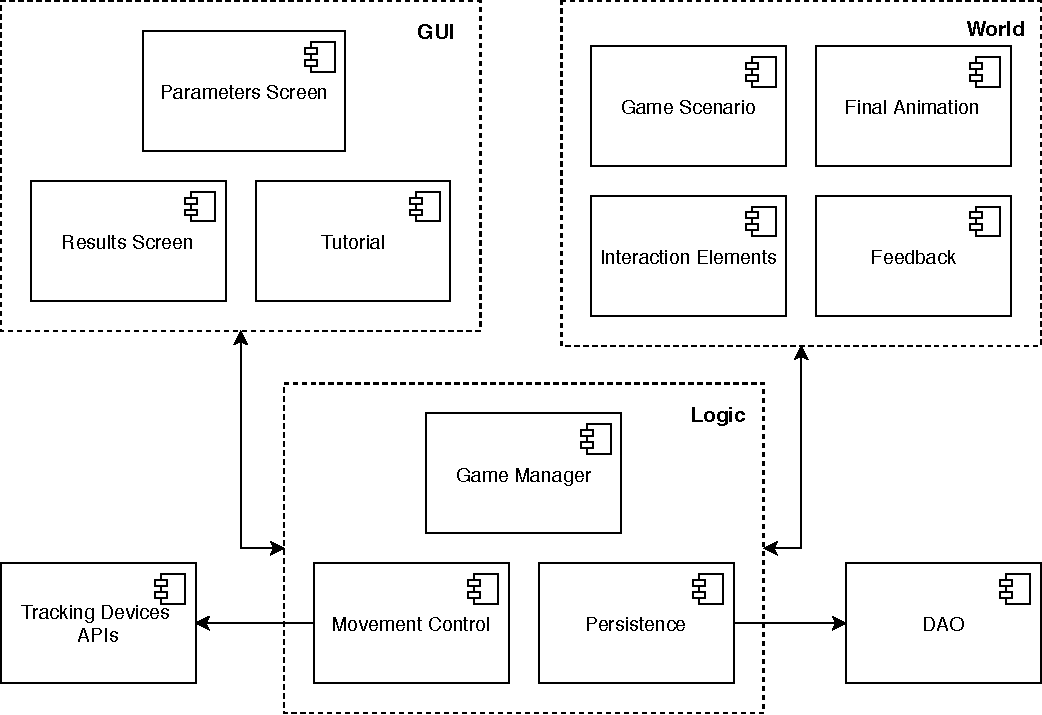
\includegraphics[width=.9\linewidth]{gfx/playtherapy/minigame_architecture}
\caption{Playtherapy's exergames architecture}
\label{fig:mg_arch}
\end{figure}

\begin{figure}[bth]
\centering
\subfloat[\textit{Piano}'s parameters screen]{
   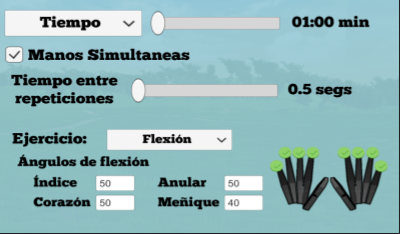
\includegraphics[width=0.4\linewidth, frame]{gfx/playtherapy/parameters_screen}
   \label{fig:parameters_screen}
}
\subfloat[\textit{Rieles}' tutorial screen]{
   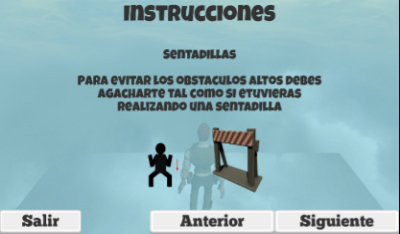
\includegraphics[width=0.4\linewidth, frame]{gfx/playtherapy/tutorial_screen}
   \label{fig:tutorial_screen}
}\\
\subfloat[\textit{Tiro Libre}'s results screen]{
   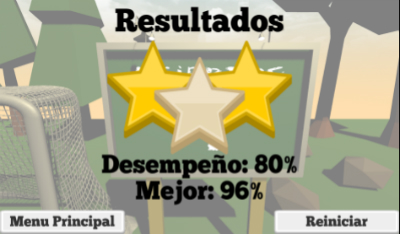
\includegraphics[width=0.4\linewidth, frame]{gfx/playtherapy/results_screen}
   \label{fig:results_screen}
 }
 \subfloat[\textit{Tiro Libre}'s game world screen]{
   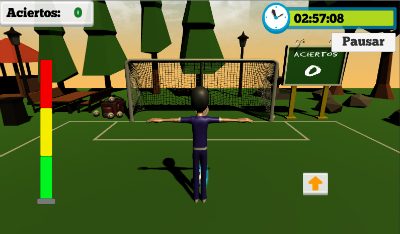
\includegraphics[width=0.4\linewidth, frame]{gfx/playtherapy/world_screen}
   \label{fig:world_screen}
}
\caption{Playtherapy's \acp{PREG} main screens}
\label{fig:platherapy_screens}
\end{figure}

Playtherapy is composed of fifteen mini-games which are briefly described below. Moreover, a characterisation of one the mini \acp{PREG} is presented in \autoref{tab:beisbol_char}, it uses the approach presented in \autoref{sec:characterising}. The characterisation for all mini \acp{PREG} is available online\footnote{\url{https://docs.google.com/spreadsheets/d/1b7AP9cNvmY6BVOT0HFJV8h7jyw7y8L7hEqteZ-woMQ0/edit\#gid=0}}.

\begin{enumerate}
    \item \emph{Tiro Libre}: players perform kick movements to strike a ball against some targets placed in a goal. It should support right/left hip flexion and extension and lateral shifts.
    \item \emph{Rieles}: players jog to go forward and squat and jump to avoid obstacles while collecting coins. It should support jumps, squats, jogging and lateral shifts.
    \item \emph{El Gran Viaje}: players control a plane moving their body to collect gems and avoid obstacles. It should support right/left hip abduction, lateral and frontal trunk inclination and squats.
    \item \emph{Estilo Libre}: players have to maintain a ball in the air using their legs. It should support right/left hip flexion and extension.
    \item \emph{Sushi Samurai}: players cut fishes coming out of the water. It should support right/left shoulder and elbow flexion and extension.
    \emph{B\'eisbol}: players have to grab balls being thrown at them using their arms. It should support right/left shoulder abduction or extension, elbow flexion and extension.
    \item \emph{Fight}: players use their arms to perform magic tricks and defend the city. It should support right/left shoulder and elbow flexion and extension.
    \item \emph{Figuras M\'agicas}: players have to draw figures using their hands to eliminate approaching enemies. It should assist in hand-eye coordination.
    \item \emph{Piano}: players have to perform finger movements to play a piano keyboard. It should support fingers flexion, extension and oppositions.
    \item \emph{Topos}: players perform grabbing movements (fist) to catch moles or directly touch them by moving their hands. It should support hand touch and grab.
    \item \emph{Vecinos Invasores}: players have to defend farm animals from being abducted by destroying alien ships using their hands. It should support hand touch and fingers oppositions.
    \item \emph{Viajando en el Espacio}: players control a spaceship using their hands to collect stars and overcome obstacles. It should support ulnar and radial deviation, wrist flexion and extension and hand grab.
    \item \emph{Dulce Hogar}: players control a cat using their hands to collect stars and avoid enemies. It should support ulnar and radial deviation, wrist flexion and extension.
    \item \emph{Cavano}: players control a bowl using their hands to gather falling objects and drop them into a jar. It should support pronation and supination.
    \item \emph{Guerra Medieval}: players have to defeat enemies using hand movements. It should support ulnar and radial deviation, wrist flexion and extension and hand grab.
\end{enumerate}

\begin{table}[bth]
\myfloatalign
\resizebox{\linewidth}{!}{
\begin{tabularx}{1.2\textwidth}{p{5cm}X}
%----------------------
\toprule
\spacedlowsmallcaps{Property}
&\spacedlowsmallcaps{Value}\\\midrule
Rehabilitation type & Tight-focused \\\midrule
Assisted Tasks & Configuration, personalisation and motivation \\\midrule
Degree of autonomy & Second degree \\\midrule
Configuration and assessment & Close-loop (Online motion range measurement)\\\midrule
Input interaction device & Camera tracking: Kinect 2\\\midrule
Output interaction device & Traditional: TV screen, speakers\\\midrule
Thematic content & Imaginary\\\midrule
Type of intervention & Individual \\\midrule
Location & Physical medicine and rehabilitation unit of Evaristo Garc\'ia University Hospital\\\midrule
Movements & Right/left shoulder abduction and/or extension, elbow flexion and extension\\\midrule
Configuration parameters & Game mode, left/right shoulder selection, minimum angle and maximum angle per movement, radius (reformulated as Movement action radius), ball speed\\\midrule
Rehabilitation goal(s) & Patient increases shoulder abduction or extension range of motion\\\midrule
Health instruments & Goniometer\\\midrule
\bottomrule
\end{tabularx}}
\caption{Characterisation of \textit{B\'eisbol} mini \ac{PREG}}
\label{tab:beisbol_char}
\end{table}

Furthermore, Playtherapy has an accompanying web application composed of three main modules. The first module is concerned with patients and physiotherapists demographic data. The second module allows physiotherapists managing patients \ac{FIM}. Finally, the third module allows visualising mini-game sessions data; e.g., registered observations, progress over time and performance measurements, like the maximum range degree achieved per session. By the time this master project took place, this application was still under development and was not connected to Playtherapy \acp{PREG}; thus, it was not evaluated.

\subsubsection{Rehabilitation support}
As described in \autoref{sec:characterising} the rehabilitation support aspect comprises assessing movement support and configuration and personalisation capability. The goal of evaluating rehabilitation support is to assure that the evaluated \ac{PREG} can be used to assure patients' safety. Therefore, we performed an \emph{internal evaluation} with two members of the development team, a physiotherapy student and a programmer, who conducted ten sessions of \ac{RITE} testing.

The physiotherapy student tested all Playtherapy's \acp{PREG}. To assess \textit{configuration capability}, she tested each configuration parameter to assess whether it behaved as expected and was easy to understand. Moreover, she tested whether the expected \textit{movements were correctly mapped} and detected by each mini \ac{PREG}. Additionally, she evaluated the \textit{quality of the tutorials} assessing the content and the coverage of the associated movements regarding the game mechanics. When she identified an error or an enhancement, the programmer fixed it and the student test it again until it was correct.

The results of the \ac{RITE} evaluation were mainly improvements related to the phrasing of configuration parameters and tutorial instructions. The student assessed their clarity from the physiotherapists' and patients' point of view. Similarly, she suggested to include graphics or animations to make the instructions and movements clearer. She configured the games considering different (ad-hoc) scenarios, exploring different game modes, including and excluding movements and modifying their difficulty. While testing each scenario, she also assessed the visibility of game objects and relevance of the visual and auditory feedback related to the game goals, leading to the inclusion of visual animations and sounds (e.g., to indicate the corresponding joint to execute a certain movement).

After the internal evaluation, we conducted five evaluation sessions of one hour using the question asking protocol and involving one physiotherapist and on physiatrist of the hospital. The purpose of this evaluation stage was to validate the results of the evaluation conducted with the development team. Eight mini \acp{PREG} were tested in this evaluation; i.e., \textit{Béisbol, Fight, Tiro Libre, Guerra Medieval, Estilo Libre, Figuras Mágicas, Gran Viaje} and \textit{Vecinos Invasores}. The last eight of these mini \acp{PREG} had been tested by the physiotherapist; thus, fewer issues were identified for those.

The participants were asked to configure at least two game sessions for each mini \ac{PREG}. After configuring one game session, they played it to identify errors or improvements. The first configuration was suggested by the evaluator, and the others were proposed by the participants. During the whole process, they could express their thoughts and impressions loudly . The evaluator could ask questions when needed. We took notes of the findings during the evaluation.

Initially, \textit{Béisbol} mini \ac{PREG} had a name in English (Baseball); however, the participants suggested to use the same name in Spanish due to the low level of patients' literacy. They expressed that understanding the game name was important to understand the game. Also, they remarked that game should indicate the patients where they should position the avatar before starting the game; they suggested to include a position mark and ask patients to move towards it. Moreover, they requested to rename one of the configuration parameters from \textit{Ratio} to \textit{Action ratio} (in Spanish) for understanding purposes. This parameter indicates the distance between the thrown ball and the patients' hands, depending on its value patients should stretch their arms or perform elbow flexion and extension movements. They suggested some rephrasing for the tutorial instructions. Regarding, movement mapping correctness, all movements were mapped correctly. However, they detected that a reduced shoulder abduction could be detected as shoulder extension. Finally, they suggested to include a visual mark indicating the position where patients should catch the balls to foster correct movement executions.

Similarly, the participants suggested to rename \textit{ABC} since its original name was in English (Fight). Also, the game displayed some visual objects to determine whether the patient should perform elbow movements. However, this was not explained in the tutorial. Thus, they requested to include that information.

About \textit{Tiro Libre}' parameters screen, the participants requested to use the term coronal plane instead of frontal plane for one of the parameters. Also, they suggested to group the \textit{Lateral shifts} and \textit{Frequency} parameters visually since they are related. Additionally, they noticed that a bar that represented the final height of a kicked ball was placed horizontally and suggested position it vertically. In the tutorial, they suggested changing the figures to differentiate lateral from frontal movements. Also, the dynamic help offered by the game was not explained in the tutorial.

Regarding \textit{Guerra Medieval}, the participants suggested to visually separate two excluding parameters. Also, the screen allowed to include pronation and supination movements, however, the game mechanics do no use them. Thus, they requested to remove them. Although the players control a virtual cannon in the game, they suggested to include virtual hands to help players be conscious of the movements they are performing. Also, they identified some typos in the tutorial and suggested to include more graphical aids and reduce the amount of text.

They detected that the performance measure presented by \textit{Estilo Libre} at the of a game session was calculated incorrectly. About the tutorial, they noticed that there was no back button to read previous instructions. Moreover, they requested some rephrasing and to modify the images to differentiate lateral from frontal movements. Regarding the parameters screen, they detected that changing the value of the \textit{Dynamic help} parameter caused no effects since the dynamic help was always presented.

About \textit{Figuras Mágicas}, the participants made some suggestions about the phrasing of the tutorial instructions. Moreover, when playing by repetitions in \textit{Gran Viaje}, the participants detected that the game requested players to execute more movements than expected. Meanwhile, they suggested some rephrasing to the tutorial of \textit{Vecinos Invasores}, and requested to remove the \textit{Pinch force} parameter since force cannot be measured by the game.

\section{Interaction}
\label{sec:interaction_eval}

\section{Effects}

\section{Discussion}
After summarising the results of the conducted evaluations, the following results were obtained:

One of the key features of Playtherapy is the configuration parameters screen, available for each mini-game, which allows personalising therapy sessions by setting exergames parameters according to the needs of a patient. The feedback received from the physiotherapists was in general positive, they expressed that it was quite helpful to be able to configure a mini-game for different patients and pathologist, and the screen was easily manageable and understandable. In the evaluations with the physiatrist and the physiotherapists all the parameters were correct since the exergames behave as expected. Their recommendations were about renaming parameters, rephrasing some tutorial instructions or adding graphical explanations to the tutorials. Only one game exergame (B\'eisbol) presented an issue regarding a movement that was not correctly mapped. Those results may be because the physiotherapy student inspected each exergame during six months and all of her recommendations were attended as soon as the appeared.

Regarding patients the evaluations that involved patients. They described both exergames as a dynamic alternative to the therapy routine. They felt immersed in both exergames since they got not distracted from the rehabilitation environment. Patients expressed their motivation and eagerness to keep playing and were enthusiastic at the fact that they could play a game while completing their rehabilitation treatments. We received some recommendations about colour combinations to improve the contrast of objects, improving their visibility to patients.

Physiotherapists described Playtherapy as an assistant tool in physical rehabilitation therapies, because it represents a dynamic alternative to therapy routine, allowing patients to have fun and also being distracted from their environment. Additionally, the physiotherapists mentioned that more exergames would be helpful, including other movements to support other exercises, as more movements may provide more flexibility during therapies.

The exergames include objectives and challenges that provide rewards when completed, motivating patients to perform better at a game and also perform the exercises needed to achieve a certain goal. Moreover, every exergame provides positive feedback when performing well, and encouraging feedback when not so well. Thus, patients may feel motivated to perform therapy sessions if they know they are also going to perform an activity they like.

According to physiotherapists feedback, Playtherapy is a promising rehabilitation tool based on configuration, personalisation, and assessment. Some reasons may be: (i) each mini-game design process was driven by rehabilitation exercises, (ii) each mini-game has an associated screen parameter to allow offering a personalised session for patients, and (iii) data collected during therapy game sessions can be managed and visualised using the web application.

The obtained positive results may be a consequence of using an incremental and iterative methodology involving physiotherapy experts along the whole development process. Expert participation allowed to understand real patients and physiotherapists' needs and expectations. Consequently, an enhanced version of each exergame was developed after each evaluation, considering feedback, proposals and suggestions received from both the physiotherapy student and the physiotherapists. 

Additional evaluations of patients' motivation and engagement may be performed since current results may be due to the novelty of the employed devices. The evaluation that we have conducted allowed us to assess the antecedents and in some degree the interaction moment of \ac{PX} offered by Playtherapy. However, to assess Playtherapy comprehensively, patients should be exposed to the exergames along a whole rehabilitation treatment. Such evaluation may allow assessing the interaction and its effects in patients more properly.

\section{Conclusion}
This chapter presented a \ac{PX} evaluation of a collection of exergames called Playtherapy. We employed the methodology proposed in \autoref{ch:methodology} to perform the evaluation. As suggested by the methodology, we performed an iterative evaluation concentrating on assessing the aspects of the antecedents moment of \ac{PX}. Our initial goal was to assess the quality of Playtherapy to assure patients safety. Therefore, we concentrated on aspects such us configuration and movement mapping correctness. We only performed one evaluation session with patients to assess \ac{PX} during interaction and get a notion of its effects (mainly emotional) on patients. Thus, we need to continue performing more evaluation iterations. The case study allowed us to confirm that evaluating the three layers of abstraction and the three moments of \ac{PX} in rehabilitation exergames represents a big challenge since it takes time and effort before a single layer or moment can be covered.

%----------------------------------------------------------------------------------------
%	THESIS CONTENT - APPENDICES
%----------------------------------------------------------------------------------------

%\appendix

%\part{Appendix} % New part of the thesis for the appendix

%\include{Chapters/Chapter0A} % Appendix GDD
%\include{Chapters/Chapter0B} % Appendix SRS
%----------------------------------------------------------------------------------------
%	POST-CONTENT THESIS PAGES
%----------------------------------------------------------------------------------------

\cleardoublepage% Bibliography

\label{app:bibliography} % Reference the bibliography elsewhere with \autoref{app:bibliography}

\manualmark
\markboth{\spacedlowsmallcaps{\bibname}}{\spacedlowsmallcaps{\bibname}} 
\refstepcounter{dummy}

\addtocontents{toc}{\protect\vspace{\beforebibskip}} % Place the bibliography slightly below the rest of the document content in the table of contents
\addcontentsline{toc}{chapter}{\tocEntry{\bibname}}

%for natbib
%\bibliographystyle{plainnat}

%\bibliography{Bibliography}

%For biblatex
\printbibliography % Bibliography

%\cleardoublepage\include{FrontBackMatter/Colophon} % Colophon

%\cleardoublepage% Declaration

\refstepcounter{dummy}
\pdfbookmark[0]{Declaration}{declaration} % Bookmark name visible in a PDF viewer

\chapter*{Declaration} % Declaration section text
I hereby declare that this research work was created autonomously without using other than the stated references. All parts which are cited directly or indirectly are marked as such. This work has not been used in the same or similar forms, in parts or in total, in other examinations.

\thispagestyle{empty}

\bigskip
 
\noindent\textit{\myLocation, \myTime}

\bigskip

\begin{flushright}
\begin{tabular}{m{5cm}}
\\ \hline
\centering\myName, \today \\
\end{tabular}
\end{flushright}
 % Declaration

%----------------------------------------------------------------------------------------

\end{document}
